\begin{ccRefClass}{Aff_transformation_2<Kernel>}

\ccDefinition
The class \ccRefName\ represents two-dimensional affine transformations. 
The general form of an affine transformation is based on a homogeneous
representation of points. Thereby all transformations can be realized by
matrix multiplications. 

Multiplying the transformation matrix by a scalar does not change the
represented transformation. Therefore, any transformation represented
by a matrix with rational entries can be represented by a
transformation matrix with integer entries as well. (Multiply the
matrix with the common denominator of the rational entries.) Hence, it
is sufficient to use the number type \ccStyle{Kernel::RT} to represent
the entries of the transformation matrix.

{\cgal} offers several specialized affine transformations. Different
constructors are provided to create them. They are parameterized with
a symbolic name to denote the transformation type, followed by
additional parameters. The symbolic name tags solve ambiguities in the
function overloading and they make the code more readable, i.e., what
type of transformation is created.

Since two-dimensional points have three homogeneous coordinates, we
have a $3\times 3$ matrix ${(m_{ij})}_{i,\,j=0\ldots 2}$.

If the homogeneous representations are normalized (the homogenizing
coordinate is 1), then the upper left $2\times 2$ matrix realizes
linear transformations. In the matrix form of a translation, the
translation vector $(v_0,\,v_1,\,1)$ appears in the last column of the
matrix. The entries $m_{20}$ and $m_{21}$ are always zero and
therefore do not appear in the constructors.

\ccCreation
\ccCreationVariable{t}

\ccConstructor{Aff_transformation_2(const Identity_transformation& );}
            {introduces an identity transformation.}

\ccConstructor{Aff_transformation_2(const Translation,
                                    const Vector_2<Kernel> &v);}
            {introduces a translation by a vector $v$.}

\ccConstructor{Aff_transformation_2(const Rotation,
                             const Direction_2<Kernel> &d,
                             const Kernel::RT &num,
                             const Kernel::RT &den = RT(1));}
            {approximates the rotation over the angle indicated by direction 
             $d$, such that the differences between the sines and cosines
             of the rotation given by d and the approximating rotation
             are at most $num/den$ each.
             \ccPrecond $num/den>0$ and $d != 0$. }

\ccConstructor{Aff_transformation_2(const Rotation,
                                       const Kernel::RT &sine_rho, 
                                       const Kernel::RT &cosine_rho, 
                                       const Kernel::RT &hw = RT(1));}
            {introduces a rotation by the angle \ccStyle{rho}.
             \ccPrecond 
             $sine\_rho^2 + cosine\_rho^2 == hw^2$.}

\ccConstructor{Aff_transformation_2(const Scaling,
                                       const Kernel::RT &s,
                                       const Kernel::RT &hw = RT(1));}
            {introduces a scaling by a scale factor $s/hw$.}

\newsavebox{\arrtwo}
\newsavebox{\arrlintwo}
\newsavebox{\transvectwo}

\savebox{\arrtwo}{\small $\left(\begin{array}{ccc}
                 m_{00} & m_{01} & m_{02}\\
                 m_{10} & m_{11} & m_{12}\\
                  0     &  0     & hw
              \end{array}\right)$}

\savebox{\arrlintwo}{\small $\left(\begin{array}{cc}
                 m_{00} & m_{01}\\
                 m_{10} & m_{11}
              \end{array}\right)$}

\savebox{\transvectwo}{\small $\left(\begin{array}{c}
                 m_{02}\\
                 m_{12}
              \end{array}\right)$}

\ccConstructor{Aff_transformation_2(
                const Kernel::RT &m00, const Kernel::RT &m01, const Kernel::RT &m02,
                const Kernel::RT &m10, const Kernel::RT &m11, const Kernel::RT &m12,
                const Kernel::RT &hw = RT(1));}
            {introduces a general affine transformation in the
             \ccTexHtml{$3 \times 3$ matrix form \usebox{\arrtwo}.}%
             {3x3 matrix <IMG ALIGN=CENTER SRC="fig/arrtwo.gif"> .}
             The sub-matrix \ccTexHtml{$1\over hw$\usebox{\arrlintwo}}%
             {<span class="math">hw<SUP>-1</SUP></span> <IMG ALIGN=CENTER 
             SRC="fig/arrlintwo.gif">} contains the scaling and rotation 
             information, the vector \ccTexHtml{$1\over hw$
             \usebox{\transvectwo}}{<span class="math">hw<SUP>-1</SUP></span>
             <IMG ALIGN=CENTER SRC="fig/transvectwo.gif">}
             contains the translational part of the transformation.}

\savebox{\arrtwo}{\small $\left(\begin{array}{ccc}
                 m_{00} & m_{01} & 0\\
                 m_{10} & m_{11} & 0\\
                  0     &  0     & hw
              \end{array}\right)$}
                  
\ccConstructor{Aff_transformation_2(
                                       const Kernel::RT &m00, const Kernel::RT &m01,
                                       const Kernel::RT &m10, const Kernel::RT &m11,
                                       const Kernel::RT &hw = RT(1));}
            {introduces a general linear transformation 
             \ccTexHtml{\usebox{\arrtwo},}{<IMG ALIGN=CENTER 
               SRC="fig/arrtwo2.gif"> ,}
             i.e.\ there is no translational part.}


\ccOperations

The main thing to do with transformations is to apply them on
geometric objects. Each class \ccStyle{Class_2<Kernel>} representing
a geometric object has a member function:

\ccStyle{Class_2<Kernel>  transform(Aff_transformation_2<Kernel> t)}.


The transformation classes provide a member function \ccStyle{transform()}
for points, vectors, directions, and lines:

\ccMethod{Point_2<Kernel>  transform(const Point_2<Kernel> &p) const;}
       {}
\ccGlue
\ccMethod{Vector_2<Kernel>  transform(const Vector_2<Kernel> &p) const;}
       {}
\ccGlue
\ccMethod{Direction_2<Kernel>  transform(const Direction_2<Kernel> &p) const;}
       {}
\ccGlue
\ccMethod{Line_2<Kernel>  transform(const Line_2<Kernel> &p) const;}
       {}

\cgal\ provides function operators for these member functions:

\ccMethod{Point_2<Kernel>  operator()(const Point_2<Kernel> &p) const;}
       {}
\ccGlue
\ccMethod{Vector_2<Kernel>  operator()(const Vector_2<Kernel> &p) const;}
       {}
\ccGlue
\ccMethod{Direction_2<Kernel>  operator()(const Direction_2<Kernel> &p) const;}
       {}
\ccGlue
\ccMethod{Line_2<Kernel>  operator()(const Line_2<Kernel> &p) const;}
       {}

\ccHeading{Miscellaneous}

\ccMethod{Aff_transformation_2<Kernel> operator*(const Aff_transformation_2<Kernel> &s) const;}{composes two affine transformations.}

\ccMethod{Aff_transformation_2<Kernel>  inverse() const;}
       {gives the inverse transformation.}

%\ccMethod{Aff_transformation_2<Kernel>  transpose() const;}
%       {returns the affine transformation defined by transposing
%       the linear transformation in \ccVar\ and setting the
%       translational part to zero.}

\ccMethod{bool                 is_even() const;}
       {returns \ccStyle{true}, if the transformation is not reflecting,
        i.e.\ the determinant of the involved linear transformation is
        non-negative.}

\ccMethod{bool                 is_odd() const;}
       {returns \ccStyle{true}, if the transformation is reflecting.}


%\ccMethod{Aff_transformation_2<Kernel>  general_form() const;}
%       {returns the affine transformation in matrix form.}

The matrix entries of a matrix representation of a 
\ccStyle{Aff_transformation_2<Kernel>}
can be accessed trough the following member functions:

\ccMethod{Kernel::FT          cartesian(int i, int j) const;}
                      {}
\ccGlue
\ccMethod{Kernel::FT          m(int i, int j) const;}
       {returns entry $m_{ij}$ in a matrix representation in which $m_{22}$ is 1.}

\ccMethod{Kernel::RT          homogeneous(int i, int j) const;}
                      {}
\ccGlue
\ccMethod{Kernel::RT          hm(int i, int j) const;}
       {returns entry $m_{ij}$ in some fixed matrix representation.} 


For affine transformations  no I/O operators are defined.

%\ccImplementation
%Depending on the constructor we have different internal representations.
%This approach uses less memory and the transformation can be applied
%faster.
%
%Affine transformations offer no \ccStyle{transform()} member function
%for complex objects because they are defined in terms of  points vectors and 
%directions.  As the internal representation of a complex object
%is private the transformation code should go there.

\ccSeeAlso
\ccc{Identity_transformation}, 
\ccc{Rotation}, 
\ccc{Scaling},
\ccc{Translation} \\
\ccc{rational_rotation_approximation}

\ccExample

\begin{cprog}
  typedef Cartesian<double>        K;
  typedef Aff_transformation_2<K>  Transformation;
  typedef Point_2<K>               Point;
  typedef Vector_2<K>              Vector;
  typedef Direction_2<K>           Direction;

  Transformation rotate(ROTATION, sin(pi), cos(pi));
  Transformation rational_rotate(ROTATION,Direction(1,1), 1, 100);
  Transformation translate(TRANSLATION, Vector(-2, 0));
  Transformation scale(SCALING, 3);

  Point q(0, 1);
  q = rational_rotate(q); 

  Point p(1, 1);

  p = rotate(p); 

  p = translate(p); 

  p = scale(p);
\end{cprog} 

The same would have been achieved with

\begin{cprog}

  Transformation transform = scale * (translate * rotate);
  p = transform(Point(1.0, 1.0));
\end{cprog} 

\ccSeeAlso
\ccRefIdfierPage{CGAL::Aff_transformation_3<Kernel>} \\
\ccRefIdfierPage{CGAL::Identity_transformation} \\
\ccRefIdfierPage{CGAL::Reflection} \\
\ccRefIdfierPage{CGAL::Rotation} \\
\ccRefIdfierPage{CGAL::Scaling} \\
\ccRefIdfierPage{CGAL::Translation} \\

\end{ccRefClass} 


\begin{ccRefClass}{Aff_transformation_3<R>}

\ccDefinition
The class \ccRefName\ represents three-dimensioanl affine transformations. 
The general form of an affine transformation is based on homogeneous
representation of points. Thereby all transformations can be realized by
matrix multiplication. 

Since the general form is based on the homogeneous representation, a
transformation matrix multiplication by a scalar does not change
the represented transformation. Therefore, any transformation represented
by a matrix with rational entries can be represented by a 
transformation matrix with integer entries as well by multiplying
the matrix with the common denominator of the rational entries. 
Hence it is sufficient to have number type \ccStyle{R::RT} for the entries 
of an affine transformation.

{\cgal} offers several specialized affine transformations. 
Different constructors are provided to create them. 
They are parameterized with a symbolic name to
denote the transformation type, followed by additional parameters.
The symbolic name tags solve ambiguities in the function
overloading and they make the code more readable, i.e.\ what type
of transformation is created.

In three-dimensional space we have a $4\times 4$ matrix ($m_{ij}$).
Entries $m_{30}$, $m_{31}$, and $m_{32}$ are always zero and 
therefore do not appear in the constructors.

\ccCreation
\ccCreationVariable{t}

\ccConstructor{Aff_transformation_3(const Identity_transformation& );}
            {introduces an identity transformation.}


\ccConstructor{Aff_transformation_3(const Translation,
                                    const Vector_3<R> &v);}
            {introduces a translation by a vector $v$.}
 
\ccConstructor{Aff_transformation_3(const Scaling,
                                    const R::RT &s,
                                    const R::RT &hw = RT(1));}
            {introduces a scaling by a scale factor $s/hw$.}

\newsavebox{\arrthree}
\newsavebox{\arrlinthree}
\newsavebox{\transvecthree}

\savebox{\arrthree}{\small $\left(\begin{array}{cccc}
                 m_{00} & m_{01} & m_{02} & m_{03}\\
                 m_{10} & m_{11} & m_{12} & m_{13}\\
                 m_{20} & m_{21} & m_{22} & m_{23}\\
                  0     &  0     &      0 & hw
              \end{array}\right)$}

\savebox{\arrlinthree}{\small $\left(\begin{array}{ccc}
                 m_{00} & m_{01} & m_{02}\\
                 m_{10} & m_{11} & m_{12}\\
                 m_{20} & m_{21} & m_{22}\\
              \end{array}\right)$}

\savebox{\transvecthree}{\small $\left(\begin{array}{c}
                 m_{03}\\
                 m_{13}\\
                 m_{23}
              \end{array}\right)$}

\ccConstructor{Aff_transformation_3(
    const R::RT &m00, const R::RT &m01, const R::RT &m02, const R::RT &m03,
    const R::RT &m10, const R::RT &m11, const R::RT &m12, const R::RT &m13,
    const R::RT &m20, const R::RT &m21, const R::RT &m22, const R::RT &m23,
                const R::RT &hw = RT(1));}
            {introduces a general affine transformation of the matrix
             form \ccTexHtml{\usebox{\arrthree}.}{<IMG ALIGN=CENTER 
             SRC=arrthree.gif> .} The part \ccTexHtml{$1\over hw$
             \usebox{\arrlinthree}}{<MATH><i>hw</i><SUP>-1</SUP></MATH> 
             <IMG ALIGN=CENTER SRC=arrlinthree.gif>}
             defines the scaling and rotational part of the transformation, 
             while the vector \ccTexHtml{$1\over hw$\usebox{\transvecthree}}%
             {<MATH><i>hw</i><SUP>-1</SUP></MATH> <IMG ALIGN=CENTER 
             SRC=transvecthree.gif>} contains the translational part.}

\savebox{\arrthree}{\small $\left(\begin{array}{cccc}
                 m_{00} & m_{01} & m_{02} & 0\\
                 m_{10} & m_{11} & m_{12} & 0\\
                 m_{20} & m_{21} & m_{22} & 0\\
                  0     &  0     &  0     &hw
              \end{array}\right)$}

\ccConstructor{Aff_transformation_3(
                        const R::RT &m00, const R::RT &m01, const R::RT& m02,
                        const R::RT &m10, const R::RT &m11, const R::RT& m12,
                        const R::RT &m20, const R::RT &m21, const R::RT& m22,
                                                      const R::RT &hw = RT(1));}
            {introduces a general linear transformation of the 
             matrix form \ccTexHtml{\usebox{\arrthree},}{<IMG ALIGN=CENTER 
             SRC=arrthree2.gif> ,} i.e.\ an affine transformation without 
             translational part.}


\ccOperations

Each class \ccStyle{Class_3<R>} representing
a geometric object in 3D has a member function:

\ccStyle{Class_3<R>  transform(Aff_transformation_3<R> t)}.


The transformation classes provide a member function \ccStyle{transform()}
for points, vectors, directions, and planes:

\ccMethod{Point_3<R>  transform(const Point_3<R> &p) const;}
       {}
\ccGlue
\ccMethod{Vector_3<R>  transform(const Vector_3<R> &p) const;}
       {}
\ccGlue
\ccMethod{Direction_3<R>  transform(const Direction_3<R> &p) const;}
       {}
\ccGlue
\ccMethod{Plane_3<R>  transform(const Plane_3<R> &p) const;}
       {}

\cgal\ provides four function operators for these member functions:

\ccMethod{Point_3<R>  operator()(const Point_3<R> &p) const;}
       {}
\ccGlue
\ccMethod{Vector_3<R>  operator()(const Vector_3<R> &p) const;}
       {}
\ccGlue
\ccMethod{Direction_3<R>  operator()(const Direction_3<R> &p) const;}
       {}
\ccGlue
\ccMethod{Plane_3<R>  operator()(const Plane_3<R> &p) const;}
       {}


\ccMethod{Aff_transformation_3<R> 
          operator*(const Aff_transformation_3<R> &s) const;}
       {composes two affine transformations.}

\ccMethod{Aff_transformation_3<R>  inverse() const;}
       {gives the inverse transformation.}

%\ccMethod{Aff_transformation_3<R>  transpose() const;}
%       {returns the affine transformation defined by transposing
%       the linear transformation in \ccVar\ and setting the
%       translational part to zero.}

\ccMethod{bool                 is_even() const;}
       {returns \ccStyle{true}, if the transformation is not reflecting,
        i.e.\ the determinant of the involved linear transformation is
        non-negative.}

\ccMethod{bool                 is_odd() const;}
       {returns \ccStyle{true}, if the transformation is reflecting.}


%\ccMethod{Aff_transformation_3<R>  general_form() const;}
%       {returns the affine transformation in matrix form.}

The matrix entries of a matrix representation of a \ccStyle{Aff_transformation_3<R>}
can be accessed trough the following member functions:

\ccMethod{FT          cartesian(int i, int j) const;}
                      {}
\ccGlue
\ccMethod{FT          m(int i, int j) const;}
       {returns entry $m_{ij}$ in a matrix representation in which $m_{33}$ is 1.}

\ccMethod{RT          homogeneous(int i, int j) const;}
                      {}
\ccGlue
\ccMethod{RT          hm(int i, int j) const;}
       {returns entry $m_{ij}$ in some fixed matrix representation.} 

For affine transformations  no I/O operators are defined.

\ccSeeAlso
\ccRefIdfierPage{CGAL::Aff_transformation_2<R>} \\
\ccRefIdfierPage{CGAL::Identity_transformation} \\
\ccRefIdfierPage{CGAL::Reflection} \\
\ccRefIdfierPage{CGAL::Rotation} \\
\ccRefIdfierPage{CGAL::Scaling} \\
\ccRefIdfierPage{CGAL::Translation} \\


\end{ccRefClass} 

\begin{ccRefFunction}{are_ordered_along_line}

\ccFunction{bool are_ordered_along_line(const Point_2<R> &p, 
                            const Point_2<R> &q, 
                            const Point_2<R> &r);}
         {returns \ccStyle{true}, iff the three points are collinear and 
          \ccStyle{q} lies between \ccStyle{p} and \ccStyle{r}.
          Note that \ccStyle{true} is returned, if \ccStyle{q==p} or
          \ccStyle{q==r}.}

\ccFunction{bool are_ordered_along_line(const Point_3<R> &p, 
                                        const Point_3<R> &q, 
                                        const Point_3<R> &r);}
         {returns \ccStyle{true}, iff the three points are collinear and 
          \ccStyle{q} lies between \ccStyle{p} and \ccStyle{r}.
          Note that \ccStyle{true} is returned, if \ccStyle{q==p} or
          \ccStyle{q==r}.}

\ccSeeAlso
\ccRefIdfierPage{CGAL::are_strictly_ordered_along_line} \\
\ccRefIdfierPage{CGAL::collinear_are_ordered_along_line} \\
\ccRefIdfierPage{CGAL::collinear_are_strictly_ordered_along_line} \\


\end{ccRefFunction}


\begin{ccRefFunction}{are_strictly_ordered_along_line}

\ccFunction{bool are_strictly_ordered_along_line(const Point_2<Kernel> &p, 
                            const Point_2<Kernel> &q, 
                            const Point_2<Kernel> &r);}
         {returns \ccStyle{true}, iff the three points are collinear and 
          \ccStyle{q} lies strictly between \ccStyle{p} and \ccStyle{r}.
          Note that \ccStyle{false} is returned, if \ccStyle{q==p} or
          \ccStyle{q==r}.}

\ccFunction{bool are_strictly_ordered_along_line(const Point_3<Kernel> &p, 
                                                 const Point_3<Kernel> &q, 
                                                 const Point_3<Kernel> &r);}
         {returns \ccStyle{true}, iff the three points are collinear and 
          \ccStyle{q} lies strictly between \ccStyle{p} and \ccStyle{r}.
          Note that \ccStyle{false} is returned, if \ccStyle{q==p} or
          \ccStyle{q==r}.}

\ccSeeAlso
\ccRefIdfierPage{CGAL::are_ordered_along_line} \\
\ccRefIdfierPage{CGAL::collinear_are_ordered_along_line} \\
\ccRefIdfierPage{CGAL::collinear_are_strictly_ordered_along_line} \\



\end{ccRefFunction}


\begin{ccRefFunction}{assign}
\ccTexHtml{\ccSetThreeColumns{Orientation}{}{\hspace*{8.5cm}}}{}

\ccInclude{CGAL/Object.h}

\ccFunctionTemplate{T}{template <class T> bool assign(T& c, const Object& o);}
       {assigns \ccStyle{o} to \ccStyle{c} if \ccStyle{o}
        was constructed from an object of type \ccStyle{T}.
        Returns \ccc{true}, if the assignment was possible.}

\ccSeeAlso
\ccRefIdfierPage{CGAL::intersection} \\
\ccRefIdfierPage{CGAL::make_object} \\

\end{ccRefFunction}


\begin{ccRefClass} {Bbox_2}
\ccInclude{CGAL/Bbox_2.h}

\ccDefinition  An object \ccStyle{b} of the class \ccRefName\ is a bounding 
box in the two-dimensional Euclidean plane $\E^2$. This class is not templated.

\ccCreation
\ccCreationVariable{b}

\ccConstructor{Bbox_2(double x_min, double y_min,
                      double x_max, double y_max);}
            {introduces a bounding box \ccVar\ with lower left corner at 
             \ccStyle{(xmin, ymin)} and with upper right corner at 
             \ccStyle{(xmax, ymax)}.}


\ccOperations

\ccHidden\ccMethod{bool operator==(const Bbox_2 &c) const;}
       {Test for equality.}

\ccHidden\ccMethod{bool operator!=(const Bbox_2 &q) const;}
       {Test for inequality.}

\ccMethod{double                 xmin() const;}{}
\ccGlue
\ccMethod{double                 ymin() const;}{}
\ccGlue
\ccMethod{double                 xmax() const;}{}
\ccGlue
\ccMethod{double                 ymax() const;}{}

\ccMethod{Bbox_2              operator+(const Bbox_2 &c) const;}
       {returns a bounding box of \ccVar\ and \ccStyle{c}.}

\ccSeeAlso
\ccRefIdfierPage{CGAL::Bbox_3} \\
\ccRefIdfierPage{CGAL::do_overlap} \\

\end{ccRefClass} 

\begin{ccRefClass} {Bbox_3}

\ccInclude{CGAL/Bbox_3.h}

\ccDefinition  An object \ccStyle{b} of the class \ccRefName\ is a bounding 
box in the three-dimensional Euclidean space $\E^3$. 

\ccCreation
\ccCreationVariable{b}


\ccConstructor{Bbox_3(double x_min, double y_min, double z_min,
                         double x_max, double y_max, double z_max);}
            {introduces a bounding box \ccVar\ with lexicographically
	     smallest corner point at \ccStyle{(xmin, ymin, zmin)} 
	     lexicographically largest corner point at 
	     \ccStyle{(xmax, ymax, zmax)}.}


\ccOperations

\ccHidden\ccMethod{bool operator==(const Bbox_3 &c) const;}
       {Test for equality.}

\ccHidden\ccMethod{bool operator!=(const Bbox_3 &q) const;}
       {Test for inequality.}

\ccMethod{double                 xmin() const;}
       {}
\ccGlue
\ccMethod{double                 ymin() const;}
       {}
\ccGlue
\ccMethod{double                 zmin() const;}
       {}
\ccGlue
\ccMethod{double                 xmax() const;}
       {}
\ccGlue
\ccMethod{double                 ymax() const;}
       {}
\ccGlue
\ccMethod{double                 zmax() const;}
       {}


\ccMethod{Bbox_3              operator+(const Bbox_3 &c) const;}
       {returns a bounding box of \ccVar\ and \ccStyle{c}.}

\ccSeeAlso
\ccRefIdfierPage{CGAL::Bbox_2} \\
\ccRefIdfierPage{CGAL::do_overlap} \\


\end{ccRefClass} 

\begin{ccRefEnum}{Bounded_side}
\ccInclude{CGAL/enum.h}

\ccGlobalEnum{enum Bounded_side {ON_UNBOUNDED_SIDE, ON_BOUNDARY, ON_BOUNDED_SIDE};
}

\ccRefLabel{ON_UNBOUNDED_SIDE}  %% add label for table-of-contents in intro.tex.
\ccRefLabel{ON_BOUNDED_SIDE}  %% add label for table-of-contents in intro.tex.
\ccRefLabel{ON_BOUNDARY}  %% add label for table-of-contents in intro.tex.
\ccHtmlCrossLink{ON_UNBOUNDED_SIDE}     %% add further rules for cross referencing links
\ccHtmlCrossLink{ON_BOUNDED_SIDE}     %% add further rules for cross referencing links
\ccHtmlCrossLink{ON_BOUNDARY}     %% add further rules for cross referencing links
\ccHtmlIndexC[enum_tags]{ON_UNBOUNDED_SIDE} %% add further index entries
\ccHtmlIndexC[enum_tags]{ON_BOUNDED_SIDE} %% add further index entries
\ccHtmlIndexC[enum_tags]{ON_BOUNDARY} %% add further index entries

%\ccSeeAlso
%\ccRefConceptPage{Kernel::HasOnBoundedSide_2} \\
%\ccRefConceptPage{Kernel::HasOnBoundedSide_3} \\

\end{ccRefEnum}

\begin{ccRefClass}{Cartesian<FieldNumberType>}
\ccInclude{CGAL/Cartesian.h}

\ccDefinition
A model for a \ccc{Kernel} using Cartesian coordinates to represent the
geometric objects.

\ccRefines
\ccc{Kernel}

\ccTypes
\ccTypedef{typedef FieldNumberType FT;}{}
\ccGlue
\ccTypedef{typedef FieldNumberType RT;}{}

\ccImplementation
This model of a kernel uses reference counting.

\ccSeeAlso
\ccc{Simple_cartesian<FieldNumberType>}, \ccc{Homogeneous<RingNumberType>}
\end{ccRefClass}

\begin{ccRefFunction}{cartesian_to_homogeneous}
\ccTexHtml{\ccSetThreeColumns{Point_2< Homogeneous<RT> > }{}{\hspace*{8.5cm}}}{}

\ccInclude{CGAL/cartesian_homogeneous_conversion.h}

\ccFunction{Point_2< Homogeneous<RT> >
cartesian_to_homogeneous(const Point_2< Cartesian<RT> >& cp);}
        {converts 2d point \ccStyle{cp} with Cartesian representation  
         into a 2d point with homogeneous representation with the same
         number type.}

\ccFunction{Point_3< Homogeneous<RT> >
cartesian_to_homogeneous(const Point_3< Cartesian<RT> >& cp);}
        {converts 3d point \ccStyle{cp} with Cartesian representation  
         into a 3d point with homogeneous representation with the same
         number type.}

\ccTexHtml{\KernelRefLayout}{}

\ccSeeAlso
\ccRefIdfierPage{CGAL::Cartesian<FieldNumberType>} \\
\ccRefIdfierPage{CGAL::Cartesian_converter<K1, K2, NTConverter>} \\
\ccRefIdfierPage{CGAL::Homogeneous<RingNumberType>} \\
\ccRefIdfierPage{CGAL::Homogeneous_converter<K1, K2, RTConverter, FTConverter>} \\
\ccRefIdfierPage{CGAL::homogeneous_to_cartesian} \\
\ccRefIdfierPage{CGAL::homogeneous_to_quotient_cartesian} \\
\ccRefIdfierPage{CGAL::quotient_cartesian_to_homogeneous} \\
\ccRefIdfierPage{CGAL::Simple_cartesian<FieldNumberType>} \\
\ccRefIdfierPage{CGAL::Simple_homogeneous<RingNumberType>} \\

\end{ccRefFunction}


\begin{ccRefClass}{Circle_2<R>}

\ccDefinition

An object of type \ccRefName\ is a circle in the
two-dimensional Euclidean plane $\E^2$. The circle is oriented, i.e.\ 
its boundary has clockwise or counterclockwise \ccHtmlNoLinksFrom{orientation}. The
boundary splits $\E^2$ into a positive and a negative side, where the
positive side is to the left of the boundary. The boundary further
splits $\E^2$ into a bounded and an unbounded side. Note that the
circle can be degenerated, i.e.\ the squared radius may be zero.


% -----------------------------------------------------------------------------
\ccCreation
\ccCreationVariable{c}

\ccHidden
\ccConstructor{ Circle_2( );}{
        introduces an uninitialized variable \ccVar\ of type
        \ccClassTemplateName.}

\ccConstructor{ Circle_2( Point_2<R>  const& center, 
                               R::FT  const& squared_radius,
                               Orientation const& ori = COUNTERCLOCKWISE);}{
        introduces a variable \ccVar\ of type \ccClassTemplateName.
        It is initialized to the circle with center \ccc{center},
        squared radius \ccc{squared_radius} and \ccHtmlNoLinksFrom{orientation}
        \ccc{ori}.
        \ccPrecond \ccc{ori} $\neq$ \ccc{COLLINEAR}, and further,
                   \ccc{squared_radius} $\geq$ 0.}

\ccConstructor{ Circle_2( Point_2<R> const& p,
                          Point_2<R> const& q,
                          Point_2<R> const& r);}{
        introduces a variable \ccVar\ of type \ccClassTemplateName.
        It is initialized to the unique circle which passes through
        the points \ccc{p}, \ccc{q} and \ccc{r}. The \ccHtmlNoLinksFrom{orientation} of
        the circle is the \ccHtmlNoLinksFrom{orientation} of the point triple \ccc{p},
        \ccc{q}, \ccc{r}.
        \ccPrecond \ccc{p}, \ccc{q}, and \ccc{r} are not collinear.}

\ccConstructor{ Circle_2( Point_2<R>  const& p, 
                               Point_2<R>  const& q,
                               Orientation const& ori 
                                                    = COUNTERCLOCKWISE);}{
        introduces a variable \ccVar\ of type \ccClassTemplateName.
        It is initialized to the circle with diameter 
        $\ccTexHtml{\overline{pq}}{pq}$
        and \ccHtmlNoLinksFrom{orientation} \ccc{ori}.
        \ccPrecond \ccc{ori} $\neq$ \ccc{COLLINEAR}.}

\ccConstructor{ Circle_2( Point_2<R>  const& center,
                               Orientation const& ori
                                                    = COUNTERCLOCKWISE);}{
        introduces a variable \ccVar\ of type \ccClassTemplateName.
        It is initialized to the circle with center \ccc{center}, squared
        radius zero and \ccHtmlNoLinksFrom{orientation} \ccc{ori}.
        \ccPrecond \ccc{ori} $\neq$ \ccc{COLLINEAR}.
        \ccPostcond \ccVar.\ccc{is_degenerate()} = \ccc{true}.}

\ccHidden
\ccConstructor{ Circle_2( Circle_2<R> const&);}{
        copy constructor.}

\ccHidden
\ccMemberFunction{ Circle_2<R>& operator = ( Circle_2<R> const&);}{
        assignment.}

% -----------------------------------------------------------------------------
\ccAccessFunctions

\ccMemberFunction{Point_2<R> const& center( ) const;}{
        returns the center of \ccVar.}
\ccGlue
\ccMemberFunction{ R::FT const& squared_radius( ) const;}{
        returns the squared radius of \ccVar.}
\ccGlue
\ccMemberFunction{ Orientation const& orientation( ) const;}{
        returns the \ccHtmlNoLinksFrom{orientation} of \ccVar.}

% -----------------------------------------------------------------------------

\ccHidden\ccMemberFunction{ bool operator == ( Circle_2<R> const& circle2) const;}{
        returns \ccc{true}, iff \ccVar\ and \ccc{circle2} are equal,
        i.e.\ if they have the same center, same squared radius and
        same \ccHtmlNoLinksFrom{orientation}.}

\ccHidden\ccMemberFunction{ bool operator != ( Circle_2<R> const& circle2) const;}{
        returns \ccc{true}, iff \ccVar\ and \ccc{circle2} are not equal.}

% -----------------------------------------------------------------------------
\ccPredicates

\ccMemberFunction{ bool is_degenerate( ) const;}{
        returns \ccc{true}, iff \ccVar\ is degenerate, i.e.\
        if \ccVar\ has squared radius zero.}

\ccMemberFunction{ Oriented_side
                   oriented_side( Point_2<R> const& p) const;}{
        returns either the constant \ccc{ON_ORIENTED_BOUNDARY}, 
        \ccc{ON_POSITIVE_SIDE}, or \ccc{ON_NEGATIVE_SIDE},
        iff \ccc{p} lies on the boundary, properly on the
        positive side, or properly on the negative side
        of \ccVar, resp.}

\ccMemberFunction{ Bounded_side
                   bounded_side( Point_2<R> const& p) const;}{
        returns \ccc{ON_BOUNDED_SIDE},
        \ccc{ON_BOUNDARY}, or \ccc{ON_UNBOUNDED_SIDE}
        iff \ccc{p} lies properly inside, on the boundary, or properly
        outside of \ccVar, resp.}

%\ccMemberFunction{ bool has_on_positive_side( Point const& p) const;}{
%        returns \ccc{true}, iff \ccc{p} lies properly on the
%        positive side of \ccVar.}
%
%\ccMemberFunction{ bool has_on_negative_side( Point const& p) const;}{
%        returns \ccc{true}, iff \ccc{p} lies properly on the
%        negative side of \ccVar.}
%
%\ccMemberFunction{ bool has_on_boundary( Point const& p) const;}{
%        returns \ccc{true}, iff \ccc{p} lies on the boundary
%        of \ccVar.}
%
%\ccMemberFunction{ bool has_on_bounded_side( Point const& p) const;}{
%        returns \ccc{true}, iff \ccc{p} lies properly inside \ccVar.}
%
%\ccMemberFunction{ bool
%                   has_on_unbounded_side( Point const& p) const;}{
%        returns \ccc{true}, iff \ccc{p} lies properly outside of \ccVar.}
\ccMethod{bool has_on_positive_side(const Point_2<R> &p) const;}
       {}
\ccGlue
\ccMethod{bool has_on_negative_side(const Point_2<R> &p) const;}
       {}
\ccGlue
\ccMethod{bool has_on_boundary(const Point_2<R> &p) const;}
       {}
\ccGlue
\ccMethod{bool has_on_bounded_side(const Point_2<R> &p) const;}
       {} 
\ccGlue
\ccMethod{bool has_on_unbounded_side(const Point_2<R> &p) const;}
       {}

% -----------------------------------------------------------------------------
\ccHeading{Miscellaneous}

\ccMemberFunction{ Circle_2<R> opposite() const;}{
        returns the circle with the same center and squared radius as
        \ccVar\, but with \ccHtmlNoLinksFrom{opposite} \ccHtmlNoLinksFrom{orientation}.}


\ccMemberFunction{ Circle_2<R> orthogonal_transform(
                       Aff_transformation_2<R> const& at) const;}{
        returns the circle obtained by applying $at$ on \ccVar.
        \ccPrecond \ccc{at} is an orthogonal transformation.}

\ccMemberFunction{ Bbox_2 bbox() const;}{
        returns a bounding box containing \ccVar.}

\ccSeeAlso

\ccRefConceptPage{Kernel::Circle_2} \\

\end{ccRefClass}

\begin{ccRefFunction}{circumcenter}

\ccFunction{Point_2<R>
circumcenter( const Point_2<R>& p,
              const Point_2<R>& q,
              const Point_2<R>& r);}
 {compute the center of the circle passing through the points $p$, $q$, and $r$.
  \ccPrecond $p$, $q$, and $r$ are not collinear.}

\ccFunction{Point_3<R>
circumcenter( const Point_3<R>& p,
              const Point_3<R>& q,
              const Point_3<R>& r);}
 {compute the center of the circle passing through the points $p$, $q$, and $r$.
  \ccPrecond $p$, $q$, and $r$ are not collinear.}

\ccFunction{Point_3<R>
circumcenter( const Point_3<R>& p,
              const Point_3<R>& q,
              const Point_3<R>& r,
              const Point_3<R>& s);}
 {compute the center of the sphere passing through the points $p$, $q$, $r$, and $s$.
  \ccPrecond $p$, $q$, $r$, and $s$ are not coplanar.}
\end{ccRefFunction}


\begin{ccRefConstant}{CLOCKWISE}
\ccGlobalVariable{const Orientation CLOCKWISE = NEGATIVE;}

\ccSeeAlso
\ccRefIdfierPage{CGAL::COUNTERCLOCKWISE} \\

\end{ccRefConstant}

\begin{ccRefFunction}{cmp_dist_to_point}

\ccFunction{Comparison_result
cmp_dist_to_point(const Point_2<R>& p,
                  const Point_2<R>& q,
                  const Point_2<R>& r);}
          {compares the distances of points \ccStyle{q} and
           \ccStyle{r} to point \ccStyle{p}.
          returns \ccStyle{SMALLER}, iff \ccStyle{q} is closer
          to \ccStyle{p} than \ccStyle{r}, \ccStyle{LARGER}, iff
          \ccStyle{r} is closer to \ccStyle{p} than \ccStyle{q}, and
          \ccStyle{EQUAL} otherwise.}

\ccFunction{Comparison_result
cmp_dist_to_point(const Point_3<R>& p,
                  const Point_3<R>& q,
                  const Point_3<R>& r);}
          {compares the distances of points \ccStyle{q} and
           \ccStyle{r} to point \ccStyle{p}.
          returns \ccStyle{SMALLER}, iff \ccStyle{q} is closer
          to \ccStyle{p} than \ccStyle{r}, \ccStyle{LARGER}, iff
          \ccStyle{r} is closer to \ccStyle{p} than \ccStyle{q}, and
          \ccStyle{EQUAL} otherwise.}
\end{ccRefFunction}


\begin{ccRefFunction}{cmp_signed_dist_to_line}

\ccFunction{Comparison_result
cmp_signed_dist_to_line(const Line_2<R>&  l,
                        const Point_2<R>& p,
                        const Point_2<R>& q);}
          {returns \ccStyle{LARGER}
           iff the signed distance of \ccStyle{p} and 
           \ccStyle{l} is larger than the signed distance of \ccStyle{q}
           and \ccStyle{l}, \ccStyle{SMALLER}, iff it is smaller,
           and \ccStyle{EQUAL} iff both are equal.}

\ccFunction{Comparison_result
cmp_signed_dist_to_line(const Point_2<R>& p,
                        const Point_2<R>& q,
                        const Point_2<R>& r,
                        const Point_2<R>& s);}
	{returns \ccStyle{LARGER}
	iff the signed distance of \ccStyle{r} and 
	\ccStyle{l} is larger than the signed distance of \ccStyle{s}
	and \ccStyle{l}, \ccStyle{SMALLER}, iff it is smaller,
	and \ccStyle{EQUAL} iff both are equal, where 
        \ccc{l} is the directed line through \ccc{p} and \ccc{q}.}
\end{ccRefFunction}


\begin{ccRefFunction}{cmp_signed_dist_to_plane}

\ccFunction{Comparison_result
cmp_signed_dist_to_plane(const Plane_3<R>& h,
                         const Point_3<R>& p,
                         const Point_3<R>& q);}
          {returns \ccStyle{LARGER}
           iff the signed distance of \ccStyle{p} and 
           \ccStyle{h} is larger than the signed distance of \ccStyle{q}
           and \ccStyle{h}, \ccStyle{SMALLER}, iff it is smaller,
           and \ccStyle{EQUAL} iff both are equal.}

\ccFunction{Comparison_result
cmp_signed_dist_to_plane(const Point_3<R>& p,
                         const Point_3<R>& q,
                         const Point_3<R>& r,
                         const Point_3<R>& s,
                         const Point_3<R>& t);}
          {returns \ccStyle{LARGER}
           iff the signed distance of \ccStyle{s} and 
           \ccStyle{h} is larger than the signed distance of \ccStyle{t}
           and \ccStyle{h}, \ccStyle{SMALLER}, iff it is smaller,
           and \ccStyle{EQUAL} iff both are equal, where
           \ccc{h} is the oriented plane through \ccc{p}, \ccc{q} and
           \ccc{r}.}
         {}
\end{ccRefFunction}


\begin{ccRefConstant}{COLLINEAR}
\ccGlobalVariable{const Orientation COLLINEAR = ZERO;}

\ccSeeAlso
\ccc{CLOCKWISE},
\ccc{COUNTERCLOCKWISE}
\end{ccRefConstant}

\begin{ccRefFunction}{collinear}
\ccInclude{CGAL/predicates_on_points_2.h}

\ccFunction{bool collinear(const Point_2<R> &p, 
                           const Point_2<R> &q, 
                           const Point_2<R> &r);}
{returns \ccStyle{true}, iff $p$, $q$, and $r$ are collinear.}

\ccInclude{CGAL/predicates_on_points_3.h}

\ccFunction{bool collinear(const Point_3<R> &p,
                           const Point_3<R>&q,
                           const Point_3<R>&r);}
{returns \ccStyle{true}, iff $p$, $q$, and $r$ are collinear.}
\end{ccRefFunction}


\begin{ccRefFunction}{collinear_are_ordered_along_line}

\ccFunction{bool collinear_are_ordered_along_line(const Point_2<R> &p,
                                      const Point_2<R> &q,
                                      const Point_2<R> &r);}
         {returns \ccStyle{true}, iff \ccStyle{q} lies between \ccStyle{p} 
          and \ccStyle{r}. \ccPrecond \ccStyle{p, q} and \ccStyle{r} are 
          collinear.}

\ccFunction{bool collinear_are_ordered_along_line(const Point_3<R> &p,
                                                  const Point_3<R> &q,
                                                  const Point_3<R> &r);}
         {returns \ccStyle{true}, iff \ccStyle{q} lies between \ccStyle{p} 
          and \ccStyle{r}. \ccPrecond \ccStyle{p, q} and \ccStyle{r} are 
          collinear.}

\ccSeeAlso
\ccRefIdfierPage{CGAL::are_ordered_along_line} \\
\ccRefIdfierPage{CGAL::are_strictly_ordered_along_line} \\
\ccRefIdfierPage{CGAL::collinear_are_strictly_ordered_along_line} \\

\end{ccRefFunction}


\begin{ccRefFunction}{collinear_are_strictly_ordered_along_line}

\ccFunction{bool collinear_are_strictly_ordered_along_line(const Point_2<Kernel> &p,
                                      const Point_2<Kernel> &q,
                                      const Point_2<Kernel> &r);}
         {returns \ccStyle{true}, iff \ccStyle{q} lies strictly between 
          \ccStyle{p} and \ccStyle{r}. \ccPrecond{\ccStyle{p, q} and \ccStyle{r} are 
          collinear.}}

\ccFunction{bool collinear_are_strictly_ordered_along_line(
                                      const Point_3<Kernel> &p,
                                      const Point_3<Kernel> &q,
                                      const Point_3<Kernel> &r);}
         {returns \ccStyle{true}, iff \ccStyle{q} lies strictly between \ccStyle{p} 
          and \ccStyle{r}. \ccPrecond{\ccStyle{p, q} and \ccStyle{r} are 
          collinear.}}

\ccSeeAlso

\ccRefIdfierPage{CGAL::are_ordered_along_line} \\
\ccRefIdfierPage{CGAL::are_strictly_ordered_along_line} \\
\ccRefIdfierPage{CGAL::collinear_are_ordered_along_line} \\

\end{ccRefFunction}


\begin{ccRefFunction}{compare_lexicographically_xy}

\ccFunction{Comparison_result
compare_lexicographically_xy(const Point_2<R>& p,
                             const Point_2<R>& q);}
      {Compares the Cartesian coordinates of points \ccStyle{p} and
       \ccStyle{q} lexicographically in $xy$ order: first 
       $x$-coordinates are compared, if they are equal, $y$-coordinates
       are compared.}
\end{ccRefFunction}


\begin{ccRefFunction}{compare_lexicographically_xyz}

\ccFunction{Comparison_result
compare_lexicographically_xyz(const Point_3<R>& p,
                              const Point_3<R>& q);}
      {Compares the Cartesian coordinates of points \ccStyle{p} and
       \ccStyle{q} lexicographically in $xyz$ order: first 
       $x$-coordinates are compared, if they are equal, $y$-coordinates
       are compared, and if both $x$- and $y$- coordinate are equal,
       $z$-coordinates are compared.}
\end{ccRefFunction}


\begin{ccRefFunction}{compare_x}

Depending on which \cgal\ \ccHtmlNoLinksFrom{kernel} is used,
different versions of this global function are available. This is
described below.

%%%%%%%%%%%%%%%%%%%%%%%%%%%%%%%%%%%%%%%%%%%%%%
\paragraph{With the basic 2D and 3D Kernel} (see Chapter~\ref{chapter-kernel-23})

\ccFunction{Comparison_result compare_x(const Point_2<Kernel> &p,
                                        const Point_2<Kernel> &q);}
        {compares the $x$-coordinates of $p$ and $q$.}

\ccFunction{Comparison_result compare_x(const Point_3<Kernel> &p,
                                        const Point_3<Kernel> &q);}
        {compares the $x$-coordinates of $p$ and $q$.}

\begin{ccTexOnly}
\begin{figure}[hb]
\centerline{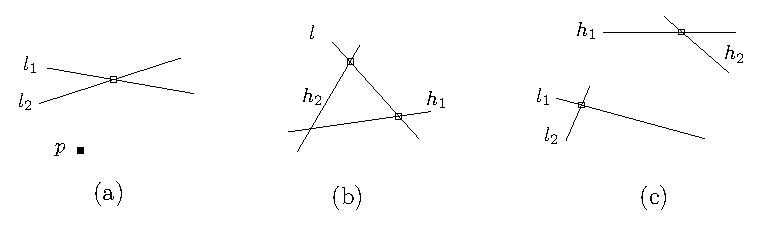
\includegraphics{Kernel_23_ref/fig/compare1}}
\caption{Comparison of the $x$ or $y$-coordinates of the (implicitly
given) points in the boxes.\label{fig-compare}}
\end{figure} 
\end{ccTexOnly} 

\ccFunction{Comparison_result compare_x(const Point_2<Kernel> &p,
                                        const Line_2<Kernel> &l1,
                                        const Line_2<Kernel> &l2);}
        {compares the $x$-coordinates of $p$ and the \ccHtmlNoLinksFrom{intersection} 
         of lines $l1$ and $l2$% 
         \ccTexHtml{ (Figure~\ref{fig-compare} (a))}{, see (a) in the figure 
         below}.}


\ccFunction{Comparison_result compare_x(const Line_2<Kernel> &l,
                                        const Line_2<Kernel> &h1,
                                        const Line_2<Kernel> &h2);}
        {compares the $x$-coordinates of  the \ccHtmlNoLinksFrom{intersection} of line $l$
         with line $h1$ and with line $h2$%
         \ccTexHtml{ (Figure~\ref{fig-compare} (b))}{, see (b) in the figure 
         below}.}


\ccFunction{Comparison_result compare_x(const Line_2<Kernel> &l1,
                                        const Line_2<Kernel> &l2,
                                        const Line_2<Kernel> &h1,
                                        const Line_2<Kernel> &h2);}
        {compares the $x$-coordinates of the \ccHtmlNoLinksFrom{intersection} of lines $l1$
         and $l2$ and  the \ccHtmlNoLinksFrom{intersection} of lines $h1$ and $h2$%
         \ccTexHtml{ (Figure~\ref{fig-compare} (c))}{, see (c) in the figure 
         below}.}

\begin{ccHtmlOnly}
<img border=0 src="fig/compare1.gif" align=middle alt="Comparison of the x 
or y coordinates of the (implicitly given) points in the boxes">
\end{ccHtmlOnly} 

%%%%%%%%%%%%%%%%%%%%%%%%%%%%%%%%%%%%%%%%%%%%%%
\paragraph{With the 2D Circular Kernel} (see Chapter~\ref{chapter-circular-kernel}) 

\ccInclude{CGAL/global_functions_circular_kernel_2.h}

If this kernel is used, in addition to the function and the
combination of 2D types described above, another version of the function
is provided.

\ccFunction{Comparison_result 
  compare_x(const Circular_arc_point_2<CircularKernel> &p,
            const Circular_arc_point_2<CircularKernel> &q);}
{compares the $x$-coordinates of $p$ and $q$.}

\ccFunction{Comparison_result 
  compare_x(const Circular_arc_point_2<CircularKernel> &p,
            const Point_2<CircularKernel> &q);}
{compares the $x$-coordinates of $p$ and $q$.}

%%%%%%%%%%%%%%%%%%%%%%%%%%%%%%%%%%%%%%%%%%%%%%
\paragraph{With the 3D Spherical Kernel} (see Chapter~\ref{chapter-spherical-kernel}) 

\ccInclude{CGAL/global_functions_spherical_kernel_3.h}

If this kernel is used, in addition to the function and the
combination of 2D types described above, another version of the function
is provided.

\ccFunction{Comparison_result 
  compare_x(const Circular_arc_point_3<SphericalKernel> &p,
            const Circular_arc_point_3<SphericalKernel> &q);}
{compares the $x$-coordinates of $p$ and $q$.}

\ccFunction{Comparison_result 
  compare_x(const Circular_arc_point_3<SphericalKernel> &p,
            const Point_3<SphericalKernel> &q);}
{compares the $x$-coordinates of $p$ and $q$.}

%%%%%%%%%%%%%%%%%%%%%%%%%%%%%%%%%%%%%%%%%%%%%
\ccSeeAlso
\ccRefIdfierPage{CGAL::compare_xy} \\
\ccRefIdfierPage{CGAL::compare_xyz} \\
\ccRefIdfierPage{CGAL::compare_x_at_y} \\
\ccRefIdfierPage{CGAL::compare_y} \\
\ccRefIdfierPage{CGAL::compare_yx} \\
\ccRefIdfierPage{CGAL::compare_y_at_x} \\
\ccRefIdfierPage{CGAL::compare_z} \\

\end{ccRefFunction}


\begin{ccRefFunction}{compare_y}

\ccFunction{Comparison_result compare_y(const Point_2<Kernel> &p,
                            	        const Point_2<Kernel> &q);}
	{compares Cartesian $y$-coordinates of $p$ and $q$.}

\ccFunction{Comparison_result compare_y(const Point_3<Kernel> &p,
                            	        const Point_3<Kernel> &q);}
	{compares Cartesian $y$-coordinates of $p$ and $q$.}

\begin{ccHtmlOnly}
<img border=0 src=./compare1.gif align=center alt="Comparison of the x 
or y coordinates of the (implicitly given) points in the boxes">
\end{ccHtmlOnly} 

\begin{ccTexOnly}
\begin{figure}[hb]
\centerline{\Ipe{compare1.ipe}}
\caption{Comparison of the $x$ or $y$-coordinates of the (implicitly
given) points in the boxes.\label{fig-compare13}}
\end{figure} 
\end{ccTexOnly} 

\ccFunction{Comparison_result compare_y(const Point_2<Kernel> &p,
                                        const Line_2<Kernel> &l1,
                                        const Line_2<Kernel> &l2);}
        {compares the $y$-coordinates of $p$ and the \ccHtmlNoLinksFrom{intersection} of lines
         $l1$ and $l2$%
         \ccTexHtml{ (Figure~\ref{fig-compare13} (a))}{, see (a) in the figure 
         above}.}


\ccFunction{Comparison_result compare_y(const Line_2<Kernel> &l,
                                        const Line_2<Kernel> &h1,
                                        const Line_2<Kernel> &h2);}
        {compares the $y$-coordinates of the \ccHtmlNoLinksFrom{intersection} of line $l$
         with line $h1$ and with line $h2$%
         \ccTexHtml{ (Figure~\ref{fig-compare13} (b))}{, see (b) in the figure 
         above}.}


\ccFunction{Comparison_result compare_y(const Line_2<Kernel> &l1,
                                        const Line_2<Kernel> &l2,
                                        const Line_2<Kernel> &h1,
                                        const Line_2<Kernel> &h2);}
        {compares the $y$-coordinates of the \ccHtmlNoLinksFrom{intersection} of lines $l1$
         and $l2$ and  the \ccHtmlNoLinksFrom{intersection} of lines $h1$ and $h2$ 
         \ccTexHtml{ (Figure~\ref{fig-compare13} (c))}{, see (c) in the figure 
         above}.}

\ccSeeAlso
\ccRefIdfierPage{CGAL::compare_xy} \\
\ccRefIdfierPage{CGAL::compare_xyz} \\
\ccRefIdfierPage{CGAL::compare_x} \\
\ccRefIdfierPage{CGAL::compare_x_at_y} \\
\ccRefIdfierPage{CGAL::compare_yx} \\
\ccRefIdfierPage{CGAL::compare_y_at_x} \\
\ccRefIdfierPage{CGAL::compare_z} \\

\end{ccRefFunction}


\begin{ccRefFunction}{compare_y_at_x}

Depending on which \cgal\ \ccHtmlNoLinksFrom{kernel} is used,
different versions of this global function are available. This is
described below.

%%%%%%%%%%%%%%%%%%%%%%%%%%%%%%%%%%%%%%%%%%%%%%
\paragraph{With the basic 2D and 3D Kernel} (see Chapter~\ref{chapter-kernel-23})

\ccFunction{Comparison_result compare_y_at_x(const Point_2<Kernel> &p,
                                             const Line_2<Kernel> &h);}
        {compares the $y$-coordinates of $p$ and the vertical projection
         of \ccStyle{p} on \ccStyle{h}%
         \ccTexHtml{ (Figure~\ref{fig-compare2} (d))}{, see (d) in the figure 
         below}.
         \ccPrecond \ccStyle{h} is not vertical.
         }

 \begin{ccTexOnly}
\begin{figure}[h]
\centerline{\includegraphics{Kernel_23_ref/fig/compare2}}
\caption{Comparison of the $y$-coordinates of the (implicitly given)
         points in the boxes, at an $x$-coordinate. The $x$-coordinate
         is either given explicitly (disc) or implicitly (circle).
         \label{fig-compare2}}
\end{figure} 
\end{ccTexOnly} 

\ccFunction{Comparison_result compare_y_at_x(const Point_2<Kernel> &p,
                                           const Line_2<Kernel> &h1,
                                           const Line_2<Kernel> &h2);}
{compares the $y$-coordinates of the vertical projection 
 of \ccStyle{p} on \ccStyle{h1} and on \ccStyle{h2}%
 \ccTexHtml{ (Figure~\ref{fig-compare2} (e))}{, see (e) in the figure 
 below}.
\ccPrecond \ccStyle{h1} and \ccStyle{h2} are not vertical.
}


\ccFunction{Comparison_result compare_y_at_x(const Line_2<Kernel> &l1,
                                           const Line_2<Kernel> &l2,
                                           const Line_2<Kernel> &h);}
      {Let $p$ be the \ccHtmlNoLinksFrom{intersection} of lines $l1$ and $l2$.
       This function compares the $y$-coordinates of $p$ and 
       the vertical projection of \ccStyle{p} on \ccStyle{h}%
       \ccTexHtml{ (Figure~\ref{fig-compare2} (f))}{, see (f) in the figure 
       below}.
       \ccPrecond \ccStyle{l1}, \ccStyle{l2} intersect and \ccStyle{h} is not
       vertical.
      }


\ccFunction{Comparison_result compare_y_at_x(const Line_2<Kernel> &l1,
                                           const Line_2<Kernel> &l2,
                                           const Line_2<Kernel> &h1,
                                           const Line_2<Kernel> &h2);}
{Let $p$ be the \ccHtmlNoLinksFrom{intersection} of lines $l1$ and $l2$. This function 
 compares the $y$-coordinates of the vertical projection of \ccStyle{p} on 
 \ccStyle{h1} and on \ccStyle{h2}%
 \ccTexHtml{ (Figure~\ref{fig-compare2} (g))}{, see (g) in the figure 
 below}.
 \ccPrecond \ccStyle{l1} and \ccStyle{l2} intersect; \ccStyle{h1} and 
 \ccStyle{h2} are not vertical.
}

\ccFunction{Comparison_result compare_y_at_x(const Point_2<Kernel> &p,
                                             const Segment_2<Kernel> &s);}
{compares the $y$-coordinates of $p$ and the vertical projection
 of \ccStyle{p} on \ccStyle{s}.  If \ccc{s} is vertical, then return
 \ccc{EQUAL} when \ccc{p} lies on \ccc{s}, \ccc{SMALLER} when \ccc{p} lies
 under {s}, and \ccc{LARGER} otherwise.
 \ccPrecond \ccStyle{p} is within the x range of \ccStyle{s}.}

\ccFunction{Comparison_result compare_y_at_x(const Point_2<Kernel> &p,
                                           const Segment_2<Kernel> &s1,
                                           const Segment_2<Kernel> &s2);}
{compares the $y$-coordinates of the vertical projection 
 of \ccStyle{p} on \ccStyle{s1} and on \ccStyle{s2}.  If \ccc{s1} or \ccc{s2}
 is vertical, then return \ccc{EQUAL} if they intersect, otherwise return
 \ccc{SMALLER} if \ccc{s1} lies below \ccc{s2}, and return \ccc{LARGER}
 otherwise.
 \ccPrecond \ccStyle{p} is within the x range of \ccStyle{s1} and \ccStyle{s2}.}


\begin{ccHtmlOnly}
<img border=0 src="fig/compare2.gif" align=middle alt="Comparison of y at x">
\end{ccHtmlOnly} 

%%%%%%%%%%%%%%%%%%%%%%%%%%%%%%%%%%%%%%%%%%%%%%
\paragraph{With the 2D Circular Kernel} (see Chapter~\ref{chapter-circular-kernel}) 

\ccInclude{CGAL/global_functions_circular_kernel_2.h}

If this kernel is used, in addition to the function and the
combination of 2D types described above, another version of the function
is provided.

\ccFunction{Comparison_result 
  compare_y_at_x(const Circular_arc_point_2<CircularKernel> &p, 
                 const Circular_arc_2<CircularKernel> &a);}
{Same as above, for a point and a circular arc.}

\ccFunction{Comparison_result 
  compare_y_at_x(const Circular_arc_point_2<CircularKernel> &p, 
                 const Line_arc_2<CircularKernel> &a);}
{Same as above, for a point and a line segment.}

\ccSeeAlso
\ccRefIdfierPage{CGAL::compare_xy} \\
\ccRefIdfierPage{CGAL::compare_xyz} \\
\ccRefIdfierPage{CGAL::compare_x} \\
\ccRefIdfierPage{CGAL::compare_x_at_y} \\
\ccRefIdfierPage{CGAL::compare_y} \\
\ccRefIdfierPage{CGAL::compare_yx} \\
\ccRefIdfierPage{CGAL::compare_z} \\

\end{ccRefFunction}


\begin{ccRefFunction}{compare_z}

\ccFunction{Comparison_result compare_z(const Point_3<R> &p,
                            	        const Point_3<R> &q);}
        {compares the $z$-coordinates of $p$ and $q$.}

\end{ccRefFunction}


\begin{ccRefEnum}{Comparison_result}
\ccInclude{CGAL/enum.h}

\ccGlobalEnum{enum  Comparison_result { SMALLER, EQUAL, LARGER };}

\ccRefLabel{SMALLER}
\ccRefLabel{EQUAL}
\ccRefLabel{LARGER}
\ccHtmlCrossLink{SMALLER}
\ccHtmlCrossLink{EQUAL}
\ccHtmlCrossLink{LARGER}

\end{ccRefEnum}


\input{COPLANAR.tex}
\begin{ccRefFunction}{coplanar}

\ccFunction{bool coplanar(const Point_3<Kernel> &p,
                               const Point_3<Kernel>&q,
                               const Point_3<Kernel>&r,
                               const Point_3<Kernel>&s);}
{returns \ccStyle{true}, if $p$, $q$, $r$, and $s$ are coplanar.}

\ccSeeAlso
\ccRefIdfierPage{CGAL::coplanar_orientation} \\
\ccRefIdfierPage{CGAL::coplanar_side_of_bounded_circle} \\

\end{ccRefFunction}


\begin{ccRefFunction}{coplanar_orientation}

\ccFunction{Orientation coplanar_orientation(const Point_3<R>& p,
                                 const Point_3<R>& q,
                                 const Point_3<R>& r,
                                 const Point_3<R>& s);}
         {Let $P$ be the plane defined by the points \ccc{p}, \ccc{q},
          and \ccc{r}. Note that the order defines the orientation of
          $P$. The function computes the orientation of points \ccc{p}, 
          \ccc{q}, and \ccc{s} in $P$: Iff \ccc{p}, \ccc{q}, \ccc{s} are
          collinear, \ccc{COLLINEAR} is returned. Iff $P$ and the plane 
          defined by \ccc{p}, \ccc{q}, and \ccc{s} have the same orientation, 
          \ccc{POSITIVE} is returned; otherwise \ccc{NEGATIVE} is returned.  
          \ccPrecond \ccc{p}, \ccc{q}, \ccc{r}, and \ccc{s} are coplanar and
          \ccc{p}, \ccc{q}, and \ccc{r} are not collinear.}
\end{ccRefFunction}


\begin{ccRefConstant}{COUNTERCLOCKWISE}
\ccGlobalVariable{const Orientation COUNTERCLOCKWISE = POSITIVE;}
\end{ccRefConstant}

\begin{ccRefFunction}{cross_product}

\ccFunction{Vector_3<R> cross_product( const Vector_3<R>& u, 
                                       const Vector_3<R>& v);}
       {returns the cross product of $u$ and $v$.}
\end{ccRefFunction}


\begin{ccRefConstant}{DEGENERATE}
\ccGlobalVariable{const Orientation DEGENERATE = ZERO;}
\end{ccRefConstant}

\begin{ccRefClass} {Direction_2<R>}

\ccDefinition
An object of the class \ccRefName\ is a vector in the two-dimensional 
vector space $\R^2$  where we forget about its length. They can be
viewed as unit vectors, although there is no normalization internally,
since this is error prone.  Directions are used whenever the length of
a vector does not matter. 
They also characterize a set of parallel oriented lines that have the same
orientations.  
For example, you can ask for the direction
orthogonal to an oriented plane, or the direction of an oriented line.
Further, they can be used to indicate angles. The slope of a direction
is \ccStyle{dy()/dx()}.


\ccCreation
\ccCreationVariable{d}


\ccHidden \ccConstructor{Direction_2();}
             {introduces an uninitialized direction \ccVar.}

\ccHidden \ccConstructor{Direction_2(const Direction_2<R> &d);}
            {copy constructor.}

\ccConstructor{Direction_2(const Vector_2<R> &v);}
            {introduces the direction \ccVar\ of vector $v$.}

\ccConstructor{Direction_2(const Line_2<R> &l);}
            {introduces the direction \ccVar\ of line $l$.}

\ccConstructor{Direction_2(const Ray_2<R> &r);}
            {introduces the direction \ccVar\ of ray $r$.}

\ccConstructor{Direction_2(const Segment_2<R> &s);}
            {introduces the direction \ccVar\ of segment $s$.}

\ccConstructor{Direction_2(const R::RT &x, const R::RT &y);}
            {introduces a direction \ccVar\ passing through the origin
             and the point with Cartesian coordinates $(x, y)$.}


\ccOperations
%\ccSetTwoOfThreeColumns{5cm}{4cm}
\ccSetThreeColumns{Direction_2<R> & }{}{\hspace*{7.8cm}}

\ccHidden \ccMethod{Direction_2<R> & operator=(const Direction_2<R> &e);}
        {Assignment.}

\ccMethod{R::RT delta(int i) const;}
       {returns values, such that \ccVar \ccc{== Direction_2<R>(delta(0),delta(1))}.
        \ccPrecond: $0 \leq i \leq 1$.}

\ccMethod{R::RT dx() const;}
       {returns \ccc{delta(0)}.}

\ccMethod{R::RT dy() const;}
       {returns \ccc{delta(1)}.}

There is a total order on directions. We compare the angles between the
positive $x$-axis and the directions in counterclockwise order.

\ccMethod{bool operator==(const Direction_2<R> &e) const;}
       {}
\ccGlue
\ccMethod{bool operator!=(const Direction_2<R> &e) const;}
       {}
\ccGlue
\ccMethod{bool operator<(const Direction_2<R> &e) const;}
       {}
\ccGlue
\ccMethod{bool operator>(const Direction_2<R> &e) const;}
       {}
\ccGlue
\ccMethod{bool operator<=(const Direction_2<R> &e) const;}
       {}
\ccGlue
\ccMethod{bool operator>=(const Direction_2<R> &e) const;}
       {}

Furthermore, we have

\ccMethod{bool counterclockwise_in_between(const Direction_2<R> &d1,
                                   const Direction_2<R> &d2) const;}
       {returns true, iff \ccVar\ is not equal to \ccc{d1}, and 
        while rotating counterclockwise starting at \ccc{d1}, 
        \ccVar\ is reached strictly before \ccc{d2} is reached.
        Note that true is returned if \ccc{d1} == \ccc{d2}, unless
        also \ccVar\ == \ccc{d1}.
       }


\ccMethod{Direction_2<R>  operator-() const;}
       {The direction opposite to \ccVar.}

\ccHeading{Miscellaneous}

\ccMethod{Vector_2<R> vector() const;}
       {returns a vector that has the same direction as \ccVar.}

\ccMethod{Direction_2<R>  transform(const Aff_transformation_2<R> &t) const;}
       {returns the direction obtained by applying $t$ on \ccVar.}

\ccSeeAlso
\ccRefConceptPage{Kernel::Direction_2} \\

\end{ccRefClass} 


\begin{ccRefClass}{Direction_3<R>}

\ccDefinition
An object of the class \ccRefName\ is a vector in the three-dimensional 
vector space $\R^3$  where we forget about their length. They can be
viewed as unit vectors, although there is no normalization internally,
since this is error prone.  Directions are used whenever the length of
a vector does not matter. 
They also characterize a set of parallel lines that have the same orientation 
or the direction normal to parallel planes that have the same orientation.
For example, you can ask for the direction
orthogonal to an oriented plane, or the direction of an oriented line.


\ccCreation
\ccCreationVariable{d}


\ccHidden \ccConstructor{Direction_3();}
             {introduces an uninitialized direction \ccVar.}

\ccHidden \ccConstructor{Direction_3(const Direction_3<R> &d);}
            {copy constructor.}

\ccConstructor{Direction_3(const Vector_3<R> &v);}
            {introduces a direction \ccVar\ initialised with the 
             direction of vector $v$.}

\ccConstructor{Direction_3(const Line_3<R> &l);}
            {introduces the direction \ccVar\ of line $l$.}

\ccConstructor{Direction_3(const Ray_3<R> &r);}
            {introduces the direction \ccVar\ of ray $r$.}

\ccConstructor{Direction_3(const Segment_3<R> &s);}
            {introduces the direction \ccVar\ of segment $s$.}

\ccConstructor{Direction_3(const R::RT &x, const R::RT &y, const R::RT &z);}
            {introduces a direction \ccVar\ initialised with the direction 
             from the origin to the point with Cartesian coordinates $(x, y, z)$.}


\ccOperations
%\ccSetTwoOfThreeColumns{5cm}{4cm}
\ccSetThreeColumns{Direction_3<R> & }{}{\hspace*{7.8cm}}

\ccHidden \ccMethod{Direction_3<R> & operator=(const Direction_3<R> &e);}
        {Assignment.}

\ccMethod{R::RT delta(int i) const;}
       {returns values, such that \ccVar \ccc{== Direction_3<R>(delta(0),delta(1),delta(2))}.
        \ccPrecond: $0 \leq i \leq 2$.}

\ccMethod{R::RT dx() const;}
       {returns \ccc{delta(0)}.}
\ccGlue
\ccMethod{R::RT dy() const;}
       {returns \ccc{delta(1)}.}
\ccGlue
\ccMethod{R::RT dz() const;}
       {returns \ccc{delta(2)}.}


\ccMethod{bool operator==(const Direction_3<R> &e) const;}
       {Test for equality.}
\ccGlue
\ccMethod{bool operator!=(const Direction_3<R> &e) const;}
       {Test for inequality.}


\ccMethod{Direction_3<R>  operator-() const;}
       {The direction opposite to \ccVar.}

\ccMethod{Vector_3<R> vector() const;}
       {returns a vector that has the same direction as \ccVar.}

\ccMethod{Direction_3<R>  transform(const Aff_transformation_3<R> &t) const;}
       {returns the direction obtained by applying $t$ on \ccVar.}

\ccSeeAlso
\ccRefConceptPage{Kernel::Direction_3}

\end{ccRefClass} 


\begin{ccRefFunction}{do_overlap}
\ccInclude{CGAL/Bbox_2.h}

\ccFunction{bool do_overlap(const Bbox_2 &bb1, const Bbox_2 &bb2);}
       {returns \ccc{true} iff \ccc{bb1} and \ccc{bb2} overlap, i.e.,
        iff their \ccHtmlNoLinksFrom{intersection} is non-empty.}

\ccInclude{CGAL/Bbox_3.h}

\ccFunction{bool do_overlap(const Bbox_3 &bb1, const Bbox_3 &bb2);}
       {returns \ccc{true} iff \ccc{bb1} and \ccc{bb2} overlap, i.e.,
        iff their \ccHtmlNoLinksFrom{intersection} is non-empty.}
\end{ccRefFunction}


\input{has_larger_dist_to_point.tex}
\begin{ccRefFunction}{has_larger_signed_dist_to_line}

\ccFunction{bool
has_larger_signed_dist_to_line(const Line_2<R>&  l,
                               const Point_2<R>& p,
                               const Point_2<R>& q);}
          {returns \ccStyle{true} iff the signed distance of \ccStyle{p}
           and \ccStyle{l} is larger than the signed distance of 
           \ccStyle{q} and \ccStyle{l}.}

\ccFunction{bool
has_larger_signed_dist_to_line(const Point_2<R>& p,
                               const Point_2<R>& q,
                               const Point_2<R>& r,
                               const Point_2<R>& s);}
          {returns \ccStyle{true} iff the signed distance of \ccStyle{r}
           and \ccStyle{l} is larger than the signed distance of 
           \ccStyle{s} and \ccStyle{l}, where \ccc{l} is the directed line
           through points \ccc{p} and \ccc{q}.}


\end{ccRefFunction}


\input{has_larger_signed_dist_to_plane.tex}
\begin{ccRefFunction}{has_smaller_dist_to_point}
\ccInclude{CGAL/distance_predicates_2.h}

\ccFunction{bool
has_smaller_dist_to_point(const Point_2<R>& p,
                          const Point_2<R>& q,
                          const Point_2<R>& r);}
         {returns \ccStyle{true} iff the distance between \ccStyle{q}
          and \ccStyle{p} is smaller than the distance between \ccStyle{r}
          and \ccStyle{p}.}

\ccInclude{CGAL/distance_predicates_3.h}

\ccFunction{bool
has_smaller_dist_to_point(const Point_3<R>& p,
                          const Point_3<R>& q,
                          const Point_3<R>& r);}
         {returns \ccStyle{true} iff the distance between \ccStyle{q}
          and \ccStyle{p} is smaller than the distance between \ccStyle{r}
          and \ccStyle{p}.}
\end{ccRefFunction}


\begin{ccRefFunction}{has_smaller_signed_dist_to_line}

\ccFunction{bool
has_smaller_signed_dist_to_line(const Line_2<R>&  l,
                                const Point_2<R>& p,
                                const Point_2<R>& q);}
          {returns \ccStyle{true} iff the signed distance of \ccStyle{p}
           and \ccStyle{l} is smaller than the signed distance of 
           \ccStyle{q} and \ccStyle{l}.}

\ccFunction{bool
has_smaller_signed_dist_to_line(const Point_2<R>& p,
                                const Point_2<R>& q,
                                const Point_2<R>& r,
                                const Point_2<R>& s);}
          {returns \ccStyle{true} iff the signed distance of \ccStyle{r}
           and \ccStyle{l} is smaller than the signed distance of 
           \ccStyle{s} and \ccStyle{l}, where \ccc{l} is the 
           oriented line through \ccc{p} and \ccc{q}.}
\end{ccRefFunction}


\begin{ccRefFunction}{has_smaller_signed_dist_to_plane}

\ccFunction{bool
has_smaller_signed_dist_to_plane(const Plane_3<R>& h,
                                 const Point_3<R>& p,
                                 const Point_3<R>& q);}
          {returns \ccStyle{true} iff the signed distance of \ccStyle{p}
           and \ccStyle{h} is smaller than the signed distance of 
           \ccStyle{q} and \ccStyle{h}.}

\ccFunction{bool
has_smaller_signed_dist_to_plane(const Point_3<R>& p,
                                 const Point_3<R>& q,
                                 const Point_3<R>& r,
                                 const Point_3<R>& s,
                                 const Point_3<R>& t);}
          {returns \ccStyle{true} iff the signed distance of \ccStyle{p}
           and \ccStyle{h} is smaller than the signed distance of 
           \ccStyle{q} and \ccStyle{h}, where \ccc{h} is the oriented
           plane through \ccc{p}, \ccc{q} and \ccc{r}.}
\end{ccRefFunction}


\begin{ccRefClass}{Homogeneous<RingNumberType>}
\ccInclude{CGAL/Homogeneous.h}

\ccDefinition
A model for a \ccc{Kernel} using homogeneous coordinates to represent the
geometric objects.  In order for \ccRefName\ to model Euclidean geometry
in $E^2$ and/or $E^3$, for some mathematical ring $E$ (\textit{e.g.},
the integers \Z\ or the rationals \Q), the template parameter \ccc{RingNumberType}
must model the mathematical ring $E$.  That is, the ring operations on this
number type must compute the mathematically correct results.  If the number
type provided as a model for \ccc{RingNumberType} is only an approximation of a
ring (such as the built-in type \ccc{double}), then the geometry provided by
the kernel is only an approximation of Euclidean geometry.  

\ccIsModel
\ccRefConceptPage{Kernel}

\ccTexHtml{\ccSetThreeColumns{typedef Quotient<RingNumberType>}{}{\hspace*{8.5cm}}}{}
\ccTypes
\ccTypedef{typedef Quotient<RingNumberType> FT;}{}
\ccGlue
\ccTypedef{typedef RingNumberType RT;}{}

\ccImplementation
This model of a kernel uses reference counting.

\ccSeeAlso
\ccRefIdfierPage{CGAL::Cartesian<FieldNumberType>} \\
\ccRefIdfierPage{CGAL::Simple_cartesian<FieldNumberType>} \\
\ccRefIdfierPage{CGAL::Simple_homogeneous<RingNumberType>} \\

\end{ccRefClass}

\begin{ccRefFunction}{homogeneous_to_cartesian}
\ccTexHtml{\ccSetThreeColumns{Point_2< Homogeneous<RT> > }{}{\hspace*{8.5cm}}}{}

\ccInclude{CGAL/cartesian_homogeneous_conversion.h}

\ccFunction{Point_2< Cartesian<FT> >
homogeneous_to_cartesian(const Point_2< Homogeneous<FT> >& hp);}
        {converts 2d point \ccStyle{hp} with homogeneous representation  
         into a 2d point with Cartesian representation with the same
         number type.}

\ccFunction{Point_3< Cartesian<FT> >
homogeneous_to_cartesian(const Point_3< Homogeneous<FT> >& hp);}
        {converts 3d point \ccStyle{hp} with homogeneous representation  
         into a 3d point with Cartesian representation with the same
         number type.}
\end{ccRefFunction}


\begin{ccRefFunction}{homogeneous_to_quotient_cartesian}

\ccInclude{CGAL/cartesian_homogeneous_conversion.h}

\ccFunction{Point_2< Cartesian<Quotient<RT> > >
homogeneous_to_quotient_cartesian(
  const Point_2<Homogeneous<RT> >& hp);}
        {converts the 2d point \ccStyle{hp} with homogeneous representation  
         with number type \ccStyle{RT} into a 2d point with Cartesian 
         representation with number type \ccStyle{Quotient<RT>}.}

\ccFunction{Point_3< Cartesian<Quotient<RT> > >
homogeneous_to_quotient_cartesian(
  const Point_3<Homogeneous<RT> >& hp);}
        {converts the 3d point \ccStyle{hp} with homogeneous representation  
         with number type \ccStyle{RT} into a 3d point with Cartesian 
         representation with number type \ccStyle{Quotient<RT>}.}

\ccSeeAlso

\ccRefIdfierPage{CGAL::Cartesian<FieldNumberType>} \\
\ccRefIdfierPage{CGAL::Cartesian_converter<K1, K2, NTConverter>} \\
\ccRefIdfierPage{CGAL::cartesian_to_homogeneous} \\
\ccRefIdfierPage{CGAL::Homogeneous<RingNumberType>} \\
\ccRefIdfierPage{CGAL::Homogeneous_converter<K1, K2, RTConverter, FTConverter>} \\
\ccRefIdfierPage{CGAL::homogeneous_to_cartesian} \\
\ccRefIdfierPage{CGAL::quotient_cartesian_to_homogeneous} \\
\ccRefIdfierPage{CGAL::Simple_cartesian<FieldNumberType>} \\
\ccRefIdfierPage{CGAL::Simple_homogeneous<RingNumberType>} \\


\end{ccRefFunction}


\begin{ccRefClass}{Identity_transformation}
\ccInclude{CGAL/aff_transformation_tags.h}

\ccDefinition
Tag class for affine transformations.

\ccSeeAlso
\ccRefIdfierPage{CGAL::Aff_transformation_2<R>} \\
\ccRefIdfierPage{CGAL::Aff_transformation_3<R>} \\
\ccRefIdfierPage{CGAL::Reflection} \\
\ccRefIdfierPage{CGAL::Rotation} \\
\ccRefIdfierPage{CGAL::Scaling} \\
\ccRefIdfierPage{CGAL::Translation} \\

\end{ccRefClass}

\begin{ccRefClass} {Iso_rectangle_2<Kernel>}

\ccDefinition  An object $s$ of the data type \ccRefName\ is a
rectangle in the Euclidean plane $\E^2$ with sides parallel to the $x$ and
$y$ axis of the coordinate system.
 
Although they are represented in a canonical form by only two
vertices, namely the lower left and the upper right vertex, we provide
functions for ``accessing'' the other vertices as well. The vertices
are returned in counterclockwise order.

Iso-oriented rectangles and bounding boxes are quite similar. The
difference however is that bounding boxes have always double coordinates, 
whereas the coordinate type of an iso-oriented rectangle is chosen by
the user.

\ccCreation
\ccCreationVariable{r}


\ccHidden \ccConstructor{Iso_rectangle_2();}
             {introduces an uninitialized variable \ccVar.}

\ccHidden \ccConstructor{Iso_rectangle_2(const Iso_rectangle_2<Kernel> &u);}
            {copy constructor.}

\ccConstructor{Iso_rectangle_2(const Point_2<Kernel> &p, 
                               const Point_2<Kernel> &q);}
            {introduces an iso-oriented rectangle \ccVar\ with diagonal
             opposite vertices $p$ and $q$. Note that the object is 
             brought in the canonical form.}

\ccConstructor{Iso_rectangle_2(const Point_2<Kernel> &p, 
                               const Point_2<Kernel> &q,
                               int);}
            {introduces an iso-oriented rectangle \ccVar\ with diagonal
             opposite vertices $p$ and $q$.  The \ccc{int} argument value
             is only used to distinguish the two overloaded functions.
             \ccPrecond{$p.x()<=q.x()$ and $p.y()<=q.y()$.}}


\ccConstructor{Iso_rectangle_2(const Point_2<Kernel> &left, 
                               const Point_2<Kernel> &right,
                               const Point_2<Kernel> &bottom,
                               const Point_2<Kernel> &top);}
            {introduces an iso-oriented rectangle \ccVar\ whose
             minimal $x$ coordinate is the one of \ccc{left}, the
             maximal $x$ coordinate is the one of \ccc{right}, the
             minimal $y$ coordinate is the one of \ccc{bottom}, the
             maximal $y$ coordinate is the one of \ccc{top}.}

\ccConstructor{Iso_rectangle_2(const Kernel::RT& min_hx, const Kernel::RT& min_hy, 
                               const Kernel::RT& max_hx, const Kernel::RT& max_hy, 
                               const Kernel::RT& hw = RT(1));}
            {introduces an iso-oriented rectangle \ccVar\ with diagonal
             opposite vertices (\ccc{min_hx/hw}, \ccc{min_hy/hw}) and 
             (\ccc{max_hx/hw}, \ccc{max_hy/hw}).  
             \ccPrecond \ccc{hw} $\neq$ 0.}

\ccOperations
\ccHidden \ccMethod{Iso_rectangle_2<Kernel> & operator=(const Iso_rectangle_2<Kernel> &q);}
        {Assignment.}

\ccMethod{bool operator==(const Iso_rectangle_2<Kernel> &r2) const;}
       {Test for equality: two iso-oriented rectangles are equal, iff their
        lower left and their upper right vertices are equal.}

\ccMethod{bool operator!=(const Iso_rectangle_2<Kernel> &r2) const;}
       {Test for inequality.}

\ccMethod{Point_2<Kernel> vertex(int i) const;}
       {returns the i'th vertex modulo 4  of \ccVar\ in counterclockwise order, 
        starting with the lower left vertex.}

\ccMethod{Point_2<Kernel> operator[](int i) const;}
       {returns  \ccStyle{vertex(i)}.}

\ccMethod{Point_2<Kernel> min() const;}
       {returns the lower left vertex of \ccVar\ (= \ccStyle{vertex(0)}).}


\ccMethod{Point_2<Kernel> max() const;}
       {returns the upper right vertex of \ccVar\ (= \ccStyle{vertex(2)}).}

\ccMethod{Kernel::FT xmin() const;}
       {returns the $x$ coordinate of lower left vertex of \ccVar.}
\ccGlue
\ccMethod{Kernel::FT ymin() const;}
       {returns the $y$ coordinate of lower left vertex of \ccVar.}
\ccGlue
\ccMethod{Kernel::FT xmax() const;}
       {returns the $x$ coordinate of upper right vertex of \ccVar.}
\ccGlue
\ccMethod{Kernel::FT ymax() const;}
       {returns the $y$ coordinate of upper right vertex of \ccVar.}

\ccMethod{Kernel::FT min_coord(int i) const;}
       {returns the $i$'th \ccHtmlNoLinksFrom{Cartesian} coordinate of the
        lower left vertex of \ccVar. 
%        (\ccc{min_coord(0) == xmin()}; \ccc{min_coord(1) == ymin()})
        \ccPrecond $0 \leq i \leq 1$.}

\ccMethod{Kernel::FT max_coord(int i) const;}
       {returns the $i$'th \ccHtmlNoLinksFrom{Cartesian} coordinate of the
        upper right vertex of \ccVar. 
%        (\ccc{max_coord(0) == xmin()}; \ccc{max_coord(1) == ymin()})
        \ccPrecond $0 \leq i \leq 1$.}

\ccPredicates

\ccMethod{bool is_degenerate() const;}
       {%the iso-oriented rectangle 
        \ccVar\ is degenerate, if all vertices
        are collinear.}

\ccMethod{Bounded_side bounded_side(const Point_2<Kernel> &p) const;}
       {returns either \ccStyle{ON_UNBOUNDED_SIDE},
        \ccStyle{ON_BOUNDED_SIDE}, or the constant
        \ccStyle{ON_BOUNDARY}, 
        depending on where point $p$ is.}

\ccMethod{bool has_on_boundary(const Point_2<Kernel> &p) const;}
       {}
\ccGlue
\ccMethod{bool has_on_bounded_side(const Point_2<Kernel> &p) const;}
       {}
\ccGlue
\ccMethod{bool has_on_unbounded_side(const Point_2<Kernel> &p) const;}
       {}

\ccHeading{Miscellaneous}

\ccMethod{Kernel::FT area() const;}
       {returns the area of \ccVar. }

\ccMethod{Bbox bbox() const;}
       {returns a bounding box containing \ccVar. }

\ccMethod{Iso_rectangle_2<Kernel>  transform(const Aff_transformation_2<Kernel> &t) const;}
       {returns the iso-oriented rectangle obtained by applying $t$ on 
        the lower left and the upper right corner of \ccVar.
        \ccPrecond The angle at a rotation must be a multiple of $\pi/2$,
        otherwise the resulting rectangle does not have the same side length.
        Note that rotating about an arbitrary angle can even result in
        a degenerate  iso-oriented rectangle.}



\ccSeeAlso
\ccRefConceptPage{Kernel::IsoRectangle_2}

\end{ccRefClass} 

\begin{ccRefConcept}{Kernel}
The concept of a {\em kernel} is defined by a set of requirements on
the provision of certain types and access member functions to create 
objects of these types. The types are function object classes to be used
within the algorithms and data structures in the basic library of \cgal. 
This allows you to use any model of a kernel as a traits class in 
the \cgal\ algorithms and data structures, unless they require types 
beyond those provided by a kernel. 

%A kernel subsumes the concepts of {\em two-dimensional kernel},
%{\em three-dimensional kernel}, and {\em $d$-dimensional kernel}.

A kernel provides types, construction objects, and generalized predicates. 
The former replace constructors of the kernel classes and constructive 
procedures in the kernel. There are also function objects replacing operators, 
especially for equality testing.

\ccHasModels

\ccRefIdfierPage{CGAL::Cartesian<FieldNumberType>} \\
\ccRefIdfierPage{CGAL::Homogeneous<RingNumberType>} \\
\ccRefIdfierPage{CGAL::Simple_cartesian<FieldNumberType>} \\
\ccRefIdfierPage{CGAL::Simple_homogeneous<RingNumberType>} \\

\ccCreationVariable{kernel}

\ccTypes

\ccNestedType{FT}{a model of FieldNumberType}
\ccGlue
\ccNestedType{RT}{a model of RingNumberType}

\ccHeading{Two-dimensional Kernel}

\ccHeading{Geometric Objects}

\ccNestedType{Point_2}{a model of Kernel::Point\_2}
\ccGlue
\ccNestedType{Vector_2}{a model of Kernel::Vector\_2}
\ccGlue
\ccNestedType{Direction_2}{a model of Kernel::Direction\_2}
\ccGlue
\ccNestedType{Line_2}{a model of Kernel::Line\_2}
\ccGlue
\ccNestedType{Ray_2}{a model of Kernel::Ray\_2}
\ccGlue
\ccNestedType{Segment_2}{a model of Kernel::Segment\_2}
\ccGlue
\ccNestedType{Triangle_2}{a model of Kernel::Triangle\_2}
\ccGlue
\ccNestedType{Iso_rectangle_2}{a model of Kernel::IsoRectangle\_2}
%%\ccGlue
%%\ccNestedType{Aff_transformation_2}{}
\ccGlue
\ccNestedType{Circle_2}{a model of Kernel::Circle\_2}
\ccGlue
\ccNestedType{Object_2}{a model of Kernel::Object\_2}

\ccHeading{Constructors}

\ccNestedType{Construct_point_2}{a model of Kernel::ConstructPoint\_2}
\ccGlue
\ccNestedType{Construct_vector_2}{a model of Kernel::ConstructVector\_2}
\ccGlue
\ccNestedType{Construct_direction_2}{a model of Kernel::ConstructDirection\_2}
\ccGlue
\ccNestedType{Construct_segment_2}{a model of Kernel::ConstructSegment\_2}
\ccGlue
\ccNestedType{Construct_line_2}{a model of Kernel::ConstructLine\_2}
\ccGlue
\ccNestedType{Construct_ray_2}{a model of Kernel::ConstructRay\_2}
\ccGlue
\ccNestedType{Construct_circle_2}{a model of Kernel::ConstructCircle\_2}
\ccGlue
\ccNestedType{Construct_triangle_2}{a model of Kernel::ConstructTriangle\_2}
\ccGlue
\ccNestedType{Construct_iso_rectangle_2}{a model of Kernel::ConstructIsoRectangle\_2}
\ccGlue
\ccNestedType{Construct_object_2}{a model of Kernel::ConstructObject\_2}
%%\ccGlue
%%\ccNestedType{Construct_aff_transformation_2}{}
\ccGlue
\ccNestedType{Construct_scaled_vector_2}{a model of Kernel::ConstructScaledVector\_2}
\ccGlue
\ccNestedType{Construct_translated_point_2}{a model of Kernel::ConstructTranslatedPoint\_2}
\ccGlue
\ccNestedType{Construct_point_on_2}{a model of Kernel::ConstructPointOn\_2}
\ccGlue
\ccNestedType{Construct_projected_point_2}{a model of Kernel::ConstructProjectedPoint\_2}
\ccGlue
\ccNestedType{Construct_projected_xy_point_2}{a model of Kernel::ConstructProjectedXYPoint\_2}
%%\ccGlue
%%\ccNestedType{Construct_second_point_on_2}{}
%%\ccGlue
%%\ccNestedType{Construct_source_point_2}{}
%%\ccGlue
%%\ccNestedType{Construct_target_point_2}{}
%%\ccGlue
%%\ccNestedType{Construct_min_point_2}{}
%%\ccGlue
%%\ccNestedType{Construct_max_point_2}{}
\ccGlue
\ccNestedType{Construct_vertex_2}{a model of Kernel::ConstructVertex\_2}
%%\ccGlue
%%\ccNestedType{Construct_direction_of_line_2}{}
%%\ccGlue
%%\ccNestedType{Construct_direction_of_ray_2}{}
\ccGlue
\ccNestedType{Construct_supporting_line_2}{a model of Kernel::ConstructSupportingLine\_2}
\ccGlue
\ccNestedType{Construct_perpendicular_vector_2}{a model of Kernel::ConstructPerpendicularVector\_2}
\ccGlue
\ccNestedType{Construct_perpendicular_direction_2}{a model of Kernel::ConstructPerpendicularDirection\_2}
\ccGlue
\ccNestedType{Construct_perpendicular_line_2}{a model of Kernel::ConstructPerpendicularLine\_2}
\ccGlue
\ccNestedType{Construct_midpoint_2}{a model of Kernel::ConstructMidpoint\_2}
\ccGlue
\ccNestedType{Construct_center_2}{a model of Kernel::ConstructCenter\_2}
\ccGlue
\ccNestedType{Construct_centroid_2}{a model of Kernel::ConstructCentroid\_2}
\ccGlue
\ccNestedType{Construct_circumcenter_2}{a model of Kernel::ConstructCircumcenter\_2}
\ccGlue
\ccNestedType{Construct_bisector_2}{a model of Kernel::ConstructBisector\_2}
\ccGlue
\ccNestedType{Construct_opposite_direction_2}{a model of Kernel::ConstructOppositeDirection\_2}
\ccGlue
\ccNestedType{Construct_opposite_segment_2}{a model of Kernel::ConstructOppositeSegment\_2}
\ccGlue
\ccNestedType{Construct_opposite_ray_2}{a model of Kernel::ConstructOppositeRay\_2}
\ccGlue
\ccNestedType{Construct_opposite_line_2}{a model of Kernel::ConstructOppositeLine\_2}
\ccGlue
\ccNestedType{Construct_opposite_triangle_2}{a model of Kernel::ConstructOppositeTriangle\_2}
\ccGlue
\ccNestedType{Construct_opposite_circle_2}{a model of Kernel::ConstructOppositeCircle\_2}
\ccGlue
\ccNestedType{Construct_opposite_vector_2}{a model of Kernel::ConstructOppositeVector\_2}

If the result type is not determined, there is no \ccc{Construct_} prefix:

%%\ccNestedType{Transform_2}{}
%%\ccGlue
\ccNestedType{Intersect_2}{a model of Kernel::Intersect\_2}
\ccGlue
\ccNestedType{Assign_2}{a model of Kernel::Assign\_2}

If the result type is a number type, the prefix is \ccc{Compute_}:

%\ccNestedType{Compute_y_at_x_2}{a model of Kernel::ComputeYatX\_2}
%\ccGlue
\ccNestedType{Compute_squared_distance_2}{a model of Kernel::ComputeSquaredDistance\_2}
\ccGlue
\ccNestedType{Compute_squared_length_2}{a model of Kernel::ComputeSquaredLength\_2}
\ccGlue
\ccNestedType{Compute_squared_radius_2}{a model of Kernel::ComputeSquaredRadius\_2}
\ccGlue
\ccNestedType{Compute_area_2}{a model of Kernel::ComputeArea\_2}

\ccHeading{Generalized Predicates}

\ccNestedType{Angle_2}{a model of Kernel::Angle\_2}
\ccGlue
\ccNestedType{Equal_2}{a model of Kernel::Equal\_2}
\ccGlue
\ccNestedType{Equal_x_2}{a model of Kernel::EqualX\_2}
\ccGlue
\ccNestedType{Equal_y_2}{a model of Kernel::EqualY\_2}
\ccGlue
\ccNestedType{Less_x_2}{a model of Kernel::LessX\_2}
\ccGlue
\ccNestedType{Less_y_2}{a model of Kernel::LessY\_2}
\ccGlue
\ccNestedType{Less_xy_2}{a model of Kernel::LessXY\_2}
\ccGlue
\ccNestedType{Less_yx_2}{a model of Kernel::LessYX\_2}
\ccGlue
\ccNestedType{Compare_x_2}{a model of Kernel::CompareX\_2}
\ccGlue
\ccNestedType{Compare_x_at_y_2}{a model of Kernel::CompareXAtY\_2}
\ccGlue
\ccNestedType{Compare_y_2}{a model of Kernel::CompareY\_2}
\ccGlue
\ccNestedType{Compare_xy_2}{a model of Kernel::CompareXY\_2}
\ccGlue
\ccNestedType{Compare_y_at_x_2}{a model of Kernel::CompareYAtX\_2}
\ccGlue
\ccNestedType{Compare_distance_2}{a model of Kernel::CompareDistance\_2}
\ccGlue
\ccNestedType{Compare_angle_with_x_axis_2}{a model of Kernel::CompareAngleWithXAxis\_2}
\ccGlue
\ccNestedType{Less_distance_to_point_2}{a model of Kernel::LessDistanceToPoint\_2}
\ccGlue
\ccNestedType{Less_signed_distance_to_line_2}{a model of Kernel::LessSignedDistanceToLine\_2}
\ccGlue
\ccNestedType{Less_rotate_ccw_2}{a model of Kernel::LessRotateCCW\_2}
\ccGlue
\ccNestedType{Leftturn_2}{a model of Kernel::LeftTurn\_2}
\ccGlue
\ccNestedType{Collinear_2}{a model of Kernel::Collinear\_2}
\ccGlue
\ccNestedType{Orientation_2}{a model of Kernel::Orientation\_2}
\ccGlue
\ccNestedType{Side_of_oriented_circle_2}{a model of Kernel::SideOfOrientedCircle\_2}
\ccGlue
\ccNestedType{Side_of_bounded_circle_2}{a model of Kernel::SideOfBoundedCircle\_2}
\ccGlue
\ccNestedType{Is_horizontal_2}{a model of Kernel::IsHorizontal\_2}
\ccGlue
\ccNestedType{Is_vertical_2}{a model of Kernel::IsVertical\_2}
\ccGlue
\ccNestedType{Is_degenerate_2}{a model of Kernel::IsDegenerate\_2}
\ccGlue
\ccNestedType{Has_on_2}{a model of Kernel::HasOn\_2}
\ccGlue
\ccNestedType{Collinear_has_on_2}{a model of Kernel::CollinearHasOn\_2}
\ccGlue
\ccNestedType{Has_on_bounded_side_2}{a model of Kernel::HasOnBoundedSide\_2}
\ccGlue
\ccNestedType{Has_on_unbounded_side_2}{a model of Kernel::HasOnUnboundedSide\_2}
\ccGlue
\ccNestedType{Has_on_boundary_2}{a model of Kernel::HasOnBoundary\_2}
\ccGlue
\ccNestedType{Has_on_positive_side_2}{a model of Kernel::HasOnPositiveSide\_2}
\ccGlue
\ccNestedType{Has_on_negative_side_2}{a model of Kernel::HasOnNegativeSide\_2}
\ccGlue
\ccNestedType{Oriented_side_2}{a model of Kernel::OrientedSide\_2}
\ccGlue
\ccNestedType{Bounded_side_2}{a model of Kernel::BoundedSide\_2}
\ccGlue
\ccNestedType{Are_ordered_along_line_2 }{a model of Kernel::AreOrderedAlongLine\_2}
\ccGlue
\ccNestedType{Are_strictly_ordered_along_line_2}{a model of Kernel::AreStrictlyOrderedAlongLine\_2}
\ccGlue
\ccNestedType{Collinear_are_ordered_along_line_2}{a model of Kernel::CollinearAreOrderedAlongLine\_2}
\ccGlue
\ccNestedType{Collinear_are_strictly_ordered_along_line_2}{a model of Kernel::CollinearAreStrictlyOrderedAlongLine\_2}
\ccGlue
\ccNestedType{Counterclockwise_in_between_2}{a model of Kernel::CounterclockwiseInBetween\_2}
\ccGlue
\ccNestedType{Do_intersect_2}{a model of Kernel::DoIntersect\_2}

\ccHeading{Three-dimensional Kernel}

\ccHeading{Geometric Objects}

\ccNestedType{Point_3}{a model of Kernel::Point\_3}
\ccGlue
\ccNestedType{Vector_3}{a model of Kernel::Vector\_3}
\ccGlue
\ccNestedType{Direction_3}{a model of Kernel::Direction\_3}
\ccGlue
\ccNestedType{Iso_cuboid_3}{a model of Kernel::IsoCuboid\_3}
\ccGlue
\ccNestedType{Line_3}{a model of Kernel::Line\_3}
\ccGlue
\ccNestedType{Ray_3}{a model of Kernel::Ray\_3}
\ccGlue
\ccNestedType{Sphere_3}{a model of Kernel::Sphere\_3}
\ccGlue
\ccNestedType{Segment_3}{a model of Kernel::Segment\_3}
\ccGlue
\ccNestedType{Plane_3}{a model of Kernel::Plane\_3}
\ccGlue
\ccNestedType{Triangle_3}{a model of Kernel::Triangle\_3}
\ccGlue
\ccNestedType{Tetrahedron_3}{a model of Kernel::Tetrahedron\_3}
%%\ccGlue
%%\ccNestedType{Aff_transformation_3}{}
\ccGlue
\ccNestedType{Object_3}{a model of Kernel::Object\_3}

\ccHeading{Constructors}

\ccNestedType{Construct_point_3}{a model of Kernel::ConstructPoint\_3}
\ccGlue
\ccNestedType{Construct_vector_3}{a model of Kernel::ConstructVector\_3}
\ccGlue
\ccNestedType{Construct_direction_3}{a model of Kernel::ConstructDirection\_3}
\ccGlue
\ccNestedType{Construct_plane_3}{a model of Kernel::ConstructPlane\_3}
\ccGlue
\ccNestedType{Construct_iso_cuboid_3}{a model of Kernel::ConstructIsoCuboid\_3}
\ccGlue
\ccNestedType{Construct_line_3}{a model of Kernel::ConstructLine\_3}
\ccGlue
\ccNestedType{Construct_ray_3}{a model of Kernel::ConstructRay\_3}
\ccGlue
\ccNestedType{Construct_sphere_3}{a model of Kernel::ConstructSphere\_3}
\ccGlue
\ccNestedType{Construct_segment_3}{a model of Kernel::ConstructSegment\_3}
\ccGlue
\ccNestedType{Construct_triangle_3}{a model of Kernel::ConstructTriangle\_3}
\ccGlue
\ccNestedType{Construct_tetrahedron_3}{a model of Kernel::ConstructTetrahedron\_3}
\ccGlue
\ccNestedType{Construct_object_3}{a model of Kernel::ConstructObject\_3}
%%\ccGlue
%%\ccNestedType{Construct_aff_transformation_3}{}
\ccGlue
\ccNestedType{Construct_scaled_vector_3}{a model of Kernel::ConstructScaledVector\_3}
\ccGlue
\ccNestedType{Construct_translated_point_3}{a model of Kernel::ConstructTranslatedPoint\_3}
\ccGlue
\ccNestedType{Construct_point_on_3}{a model of Kernel::ConstructPointOn\_3}
\ccGlue
\ccNestedType{Construct_projected_point_3}{a model of Kernel::ConstructProjectedPoint\_3}
\ccGlue
\ccNestedType{Construct_lifted_point_3}{a model of Kernel::ConstructLiftedPoint\_3}
%%\ccGlue
%%\ccNestedType{Construct_second_point_on_3}{}
%%\ccGlue
%%\ccNestedType{Construct_source_point_3}{}
%%\ccGlue
%%\ccNestedType{Construct_target_point_3}{}
%%\ccGlue
%%\ccNestedType{Construct_min_point_3}{}
%%\ccGlue
%%\ccNestedType{Construct_max_point_3}{}
\ccGlue
\ccNestedType{Construct_vertex_3}{a model of Kernel::ConstructVertex\_3}
%%\ccGlue
%%\ccNestedType{Construct_direction_of_line_3}{}
%%\ccGlue
%%\ccNestedType{Construct_direction_of_ray_3}{}
\ccGlue
\ccNestedType{Construct_supporting_line_3}{a model of Kernel::ConstructSupportingLine\_3}
\ccGlue
\ccNestedType{Construct_supporting_plane_3}{a model of Kernel::ConstructSupportingPlane\_3}
\ccGlue
\ccNestedType{Construct_orthogonal_vector_3}{a model of Kernel::ConstructOrthogonalVector\_3}
\ccGlue
\ccNestedType{Construct_base_vector_3}{a model of Kernel::ConstructBaseVector\_3}
\ccGlue
\ccNestedType{Construct_perpendicular_plane_3}{a model of Kernel::ConstructPerpendicularPlane\_3}
\ccGlue
\ccNestedType{Construct_perpendicular_line_3}{a model of Kernel::ConstructPerpendicularLine\_3}
\ccGlue
\ccNestedType{Construct_midpoint_3}{a model of Kernel::ConstructMidpoint\_3}
\ccGlue
\ccNestedType{Construct_center_3}{a model of Kernel::ConstructCenter\_3}
\ccGlue
\ccNestedType{Construct_centroid_3}{a model of Kernel::ConstructCentroid\_3}
\ccGlue
\ccNestedType{Construct_circumcenter_3}{a model of Kernel::ConstructCircumcenter\_3}
\ccGlue
\ccNestedType{Construct_cross_product_vector_3}{a model of Kernel::ConstructCrossProductVector\_3}
\ccGlue
\ccNestedType{Construct_opposite_direction_3}{a model of Kernel::ConstructOppositeDirection\_3}
\ccGlue
\ccNestedType{Construct_opposite_segment_3}{a model of Kernel::ConstructOppositeSegment\_3}
\ccGlue
\ccNestedType{Construct_opposite_ray_3}{a model of Kernel::ConstructOppositeRay\_3}
\ccGlue
\ccNestedType{Construct_opposite_line_3}{a model of Kernel::ConstructOppositeLine\_3}
\ccGlue
\ccNestedType{Construct_opposite_plane_3}{a model of Kernel::ConstructOppositePlane\_3}
\ccGlue
\ccNestedType{Construct_opposite_sphere_3}{a model of Kernel::ConstructOppositeSphere\_3}
\ccGlue
\ccNestedType{Construct_opposite_vector_3}{a model of Kernel::ConstructOppositeVector\_3}

If the result type is not determined, there is no \ccc{Construct_} prefix:

%%\ccNestedType{Transform_3}{}
%%\ccGlue
\ccNestedType{Intersect_3}{a model of Kernel::Intersect\_3}
\ccGlue
\ccNestedType{Assign_3}{a model of Kernel::Assign\_3}

If the result type is a number type, the prefix is \ccc{Compute_}:

\ccNestedType{Compute_squared_area_3}{a model of Kernel::ComputeSquaredArea\_3}
\ccGlue
\ccNestedType{Compute_squared_distance_3}{a model of Kernel::ComputeSquaredDistance\_3}
\ccGlue
\ccNestedType{Compute_squared_length_3}{a model of Kernel::ComputeSquaredLength\_3}
\ccGlue
\ccNestedType{Compute_squared_radius_3}{a model of Kernel::ComputeSquaredRadius\_3}
\ccGlue
\ccNestedType{Compute_volume_3}{a model of Kernel::ComputeVolume\_3}

\ccHeading{Generalized Predicates}

\ccNestedType{Angle_3}{a model of Kernel::Angle\_3}
\ccGlue
\ccNestedType{Equal_3}{a model of Kernel::Equal\_3}
\ccGlue
\ccNestedType{Equal_x_3}{a model of Kernel::EqualX\_3}
\ccGlue
\ccNestedType{Equal_y_3}{a model of Kernel::EqualY\_3}
\ccGlue
\ccNestedType{Equal_z_3}{a model of Kernel::EqualZ\_3}
\ccGlue
\ccNestedType{Equal_xy_3}{a model of Kernel::EqualXY\_3}
\ccGlue
\ccNestedType{Less_x_3}{a model of Kernel::LessX\_3}
\ccGlue
\ccNestedType{Less_y_3}{a model of Kernel::LessY\_3}
\ccGlue
\ccNestedType{Less_z_3}{a model of Kernel::LessZ\_3}
\ccGlue
\ccNestedType{Less_xy_3}{a model of Kernel::LessXY\_3}
\ccGlue
\ccNestedType{Less_xyz_3}{a model of Kernel::LessXYZ\_3}
\ccGlue
\ccNestedType{Compare_x_3}{a model of Kernel::CompareX\_3}
\ccGlue
\ccNestedType{Compare_y_3}{a model of Kernel::CompareY\_3}
\ccGlue
\ccNestedType{Compare_z_3}{a model of Kernel::CompareZ\_3}
\ccGlue
\ccNestedType{Compare_xy_3}{a model of Kernel::CompareXY\_3}
\ccGlue
\ccNestedType{Compare_xyz_3}{a model of Kernel::CompareXYZ\_3}
\ccGlue
\ccNestedType{Less_signed_distance_to_plane_3}{a model of Kernel::LessSignedDistanceToPlane\_3}
\ccGlue
\ccNestedType{Less_distance_to_point_3}{a model of Kernel::LessDistanceToPoint\_3}
\ccGlue
\ccNestedType{Compare_distance_3}{a model of Kernel::CompareDistance\_3}
\ccGlue
\ccNestedType{Collinear_3}{a model of Kernel::Collinear\_3}
\ccGlue
\ccNestedType{Coplanar_3}{a model of Kernel::Coplanar\_3}
\ccGlue
\ccNestedType{Orientation_3}{a model of Kernel::Orientation\_3}
\ccGlue
\ccNestedType{Coplanar_orientation_3}{a model of Kernel::CoplanarOrientation\_3}
\ccGlue
\ccNestedType{Coplanar_side_of_bounded_circle_3}{a model of Kernel::CoplanarSideOfBoundedCircle\_3}
\ccGlue
\ccNestedType{Side_of_oriented_sphere_3}{a model of Kernel::SideOfOrientedSphere\_3}
\ccGlue
\ccNestedType{Side_of_bounded_sphere_3}{a model of Kernel::SideOfBoundedSphere\_3}
\ccGlue
\ccNestedType{Is_degenerate_3}{a model of Kernel::IsDegenerate\_3}
\ccGlue
\ccNestedType{Has_on_3}{a model of Kernel::HasOn\_3}
\ccGlue
\ccNestedType{Has_on_bounded_side_3}{a model of Kernel::HasOnBoundedSide\_3}
\ccGlue
\ccNestedType{Has_on_unbounded_side_3}{a model of Kernel::HasOnUnboundedSide\_3}
\ccGlue
\ccNestedType{Has_on_boundary_3}{a model of Kernel::HasOnBoundary\_3}
\ccGlue
\ccNestedType{Has_on_positive_side_3}{a model of Kernel::HasOnPositiveSide\_3}
\ccGlue
\ccNestedType{Has_on_negative_side_3}{a model of Kernel::HasOnNegativeSide\_3}
\ccGlue
\ccNestedType{Oriented_side_3}{a model of Kernel::OrientedSide\_3}
\ccGlue
\ccNestedType{Bounded_side_3}{a model of Kernel::BoundedSide\_3}
\ccGlue
\ccNestedType{Are_ordered_along_line_3 }{a model of Kernel::AreOrderedAlongLine\_3}
\ccGlue
\ccNestedType{Are_strictly_ordered_along_line_3}{a model of Kernel::AreStrictlyOrderedAlongLine\_3}
\ccGlue
\ccNestedType{Collinear_are_ordered_along_line_3}{a model of Kernel::CollinearAreOrderedAlongLine\_3}
\ccGlue
\ccNestedType{Collinear_are_strictly_ordered_along_line_3}{a model of Kernel::CollinearAreStrictlyOrderedAlongLine\_3}
\ccGlue
\ccNestedType{Do_intersect_3}{a model of Kernel::DoIntersect\_3}


\ccHeading{d-dimensional Kernel}

\ccHeading{Geometric Objects}

\ccNestedType{Point_d}{a model of Kernel::Point\_d}

\ccHeading{Constructors}

\ccNestedType{Construct_Point_d}{a model of Kernel::ConstructPoint\_d}

\ccOperations

For each of the function objects above, there must exist a member function
that requires no arguments and returns an instance of that function object.
The name of the member function is the uncapitalized name of the type
returned with the suffix \ccc{_object} appended.  For example, for the 
function object
\ccc{Kernel::ConstructVector_2} the following member function must exist:

\ccTexHtml{\ccSetThreeColumns{Kernel::Are_strictly_ordered_along_line}{}{\hspace
*{4.5cm}}}{}

\setlength{\parskip}{0pt}

\ccMemberFunction{Kernel::ConstructVector_2 construct_vector_2_object() const ;}
{}

\def\ccTagRmEigenClassName{\ccTrue}

\ccSeeAlso

\ccAnchor{../kernel_d/index.html}{\cgal\ d-dimensional Kernel manual}.

\end{ccRefConcept} 

\begin{ccRefConcept}{Kernel::Aff_transformation_2}
\ccDefinition
A type representing affine transformations in two dimensions.

\ccRefines
\ccc{CopyConstructable},
\ccc{Assignable} 

\ccSeeAlso
\ccc{Kernel::Construct_aff_transformation_2}
\end{ccRefConcept}

\begin{ccRefConcept}{Kernel::Aff_transformation_3}
\ccDefinition
A type representing affine transformations in three dimensions.

\ccRefines
\ccc{CopyConstructable},
\ccc{Assignable} 

\ccSeeAlso
\ccc{Kernel::Construct_aff_transformation_3}

\end{ccRefConcept}         


\input{Kernel::Are_ordered_along_line_2.tex}
\input{Kernel::Are_ordered_along_line_3.tex}
\input{Kernel::Are_strictly_ordered_along_line_2.tex}
\input{Kernel::Are_strictly_ordered_along_line_3.tex}
\begin{ccRefConcept}{Kernel::Circle_2}
A type representing circles in two dimensions.

\ccRefines
\ccc{CopyConstructable},
\ccc{Assignable} 

\ccSeeAlso
\ccc{Kernel::Construct_circle_2}
\end{ccRefConcept}


\input{Kernel::Collinear_2.tex}
\input{Kernel::Collinear_3.tex}
\input{Kernel::Collinear_are_ordered_along_line_2.tex}
\input{Kernel::Collinear_are_ordered_along_line_3.tex}
\input{Kernel::Collinear_are_strictly_ordered_along_line_2.tex}
\input{Kernel::Collinear_are_strictly_ordered_along_line_3.tex}
\begin{ccRefFunctionObjectConcept}{Kernel::Collinear_has_on_2}
A model for this must provide:

\ccCreationVariable{fo}

\ccMemberFunction{bool operator()(const Kernel::Ray_2& r, 
                                  const Kernel::Point_2&p);}
       {checks if point $p$ is on $r$. 
        \ccPrecond{$p$ is on the supporting line of $r$.}}

\ccMemberFunction{bool operator()(const Kernel::Segment_2& s, 
                                  const Kernel::Point_2&p);}
       {checks if point $p$ is on $s$. 
        \ccPrecond{$p$ is on the supporting line of $s$.}}

\end{ccRefFunctionObjectConcept}

\begin{ccRefFunctionObjectConcept}{Kernel::Collinear_has_on_3}
A model for this must provide:

\ccCreationVariable{fo}

\ccMemberFunction{bool operator()(const Kernel::Ray_3& r, 
                                  const Kernel::Point_3&p);}
       {checks if point $p$ is on $r$. 
        \ccPrecond{$p$ is on the supporting line of $r$.}}

\ccMemberFunction{bool operator()(const Kernel::Segment_3& s, 
                                  const Kernel::Point_3&p);}
       {checks if point $p$ is on $s$. 
        \ccPrecond{$p$ is on the supporting line of $s$.}}

\end{ccRefFunctionObjectConcept}

\input{Kernel::Compare_x_2.tex}
\input{Kernel::Compare_x_3.tex}
\input{Kernel::Compare_xy_2.tex}
\input{Kernel::Compare_xy_3.tex}
\input{Kernel::Compare_xyz_3.tex}
\input{Kernel::Compare_y_2.tex}
\begin{ccRefFunctionObjectConcept}{Kernel::Compare_y_3}
A model for this must provide:

\ccCreationVariable{fo}

\ccMemberFunction{Comparison_result operator()(const Kernel::Point_3&p, 
                                               const Kernel::Point_3&q);}
      {Compares the Cartesian $y$-coordinates of points \ccStyle{p} and
      \ccStyle{q}}

\end{ccRefFunctionObjectConcept}

\input{Kernel::Compare_y_at_x_2.tex}
\input{Kernel::Compare_z_3.tex}
\input{Kernel::Compute_squared_length_2.tex}
\input{Kernel::Compute_squared_length_3.tex}
\begin{ccRefFunctionObjectConcept}{Kernel::Compute_x_at_y_2}
A model for this must provide:

\ccCreationVariable{fo}

\ccMemberFunction{Kernel::FT operator()(const Kernel::Line_2& l,
                                        const Kernel::FT &y) const;}
       {returns the $x$-coordinate of the point at $l$ with
        given $y$-coordinate.
        \ccPrecond $l$ is not vertical.}

\end{ccRefFunctionObjectConcept}

\input{Kernel::Compute_y_at_x_2.tex}
\input{Kernel::Construct_aff_transformation_2.tex}
\input{Kernel::Construct_aff_transformation_3.tex}
\input{Kernel::Construct_bisector_2.tex}
\input{Kernel::Construct_circle_2.tex}
\input{Kernel::Construct_circumcenter_2.tex}
\input{Kernel::Construct_direction_2.tex}
\begin{ccRefFunctionObjectConcept}{Kernel::Construct_direction_3}
A model for this must provide:

\ccCreationVariable{fo}


\ccHidden \ccMemberFunction{Kernel::Direction_3 operator()();}
             {introduces an uninitialized direction .}

\ccHidden \ccMemberFunction{Kernel::Direction_3 operator()(const Kernel::Direction_3 &d);}
 	    {copy constructor.}

\ccMemberFunction{Kernel::Direction_3 operator()(const Kernel::Vector_3 &v);}
	    {introduces a direction  initialised with the 
	     direction of vector $v$.}

\ccMemberFunction{Kernel::Direction_3 operator()(const Kernel::RT &x, const Kernel::RT &y, const Kernel::RT &z);}
            {introduces a direction  initialised with the direction 
	     from the origin to the point with Cartesian coordinates $(x, y, z)$.}


\end{ccRefFunctionObjectConcept}

\begin{ccRefFunctionObjectConcept}{Kernel::Construct_direction_of_line_2}
A model for this must provide:

\ccCreationVariable{fo}

\ccMemberFunction{Kernel::Direction_2 operator()(const Kernel::Line_2&l);}
       {returns the direction of $l$.}


\end{ccRefFunctionObjectConcept}

\begin{ccRefFunctionObjectConcept}{Kernel::Construct_direction_of_line_3}
A model for this must provide:

\ccCreationVariable{fo}

\ccMemberFunction{Kernel::Direction_3 operator()(const Kernel::Line_3&l);}
       {returns the direction of $l$.}


\end{ccRefFunctionObjectConcept}

\input{Kernel::Construct_direction_of_ray_2.tex}
\input{Kernel::Construct_direction_of_ray_3.tex}
\input{Kernel::Construct_line_2.tex}
\input{Kernel::Construct_line_3.tex}
\begin{ccRefFunctionObjectConcept}{Kernel::Construct_max_point_2}
A model for this must provide:

\ccCreationVariable{fo}

\ccMemberFunction{Kernel::Point_2 operator()(const Kernel::Iso_rectangle_2& i);}
       {returns the upper right vertex of $i$).}

\ccMemberFunction{Kernel::Point_2 operator()(const Kernel::Segment_2& s);}
       {returns the point of $s$ with lexicographically largest coordinates.}

\end{ccRefFunctionObjectConcept}

\begin{ccRefFunctionObjectConcept}{Kernel::Construct_max_point_3}
A model for this must provide:

\ccCreationVariable{fo}

\ccMemberFunction{Kernel::Point_3 operator()(const Kernel::Iso_cuboid_3& c);}
       {returns the vertex of $c$ with lexicographically largest coordinates.}

\ccMemberFunction{Kernel::Point_3 operator()(const Kernel::Segment_3& s);}
       {returns the point of $s$ with lexicographically largest coordinates.}

\end{ccRefFunctionObjectConcept}

\input{Kernel::Construct_midpoint_2.tex}
\input{Kernel::Construct_midpoint_3.tex}
\input{Kernel::Construct_min_point_2.tex}
\begin{ccRefFunctionObjectConcept}{Kernel::Construct_min_point_3}
A model for this must provide:

\ccCreationVariable{fo}

\ccMemberFunction{Kernel::Point_3 operator()(const Kernel::Iso_cuboid& c);}
       {returns the vertex of $c$ with lexicographically smallest coordinates.}

\ccMemberFunction{Kernel::Point_3 operator()(const Kernel::Segment_3& s);}
       {returns the point of $s$ with lexicographically smallest coordinates.}


\end{ccRefFunctionObjectConcept}

\input{Kernel::Construct_opposite_circle_2.tex}
\begin{ccRefFunctionObjectConcept}{Kernel::Construct_opposite_line_2}
A model for this must provide:

\ccCreationVariable{fo}

\ccMemberFunction{Kernel::Line_2 operator()(const Kernel::Line_2& l);}
{returns the line representing the same set of points as $l$,
but with opposite direction.}

\end{ccRefFunctionObjectConcept}

\input{Kernel::Construct_opposite_line_3.tex}
\input{Kernel::Construct_opposite_plane_3.tex}
\input{Kernel::Construct_opposite_ray_2.tex}
\begin{ccRefFunctionObjectConcept}{Kernel::Construct_opposite_ray_3}
A model for this must provide:

\ccCreationVariable{fo}

\ccMemberFunction{Kernel::Ray_3 operator()(const Kernel::Ray_3& r);}
{returns the ray with the same source as $r$, but in opposite direction.}

\end{ccRefFunctionObjectConcept}

\input{Kernel::Construct_opposite_segment_2.tex}
\input{Kernel::Construct_opposite_segment_3.tex}
\begin{ccRefFunctionObjectConcept}{Kernel::Construct_opposite_triangle_2}
A model for this must provide:

\ccCreationVariable{fo}

\ccMemberFunction{Kernel::Triangle_2 operator()(const Kernel::Triangle_2& t);}
       {returns the triangle with opposite orientation to $t$
        (this flips the positive and the negative side, but
        not bounded and unbounded side).}

\end{ccRefFunctionObjectConcept}

%\input{Kernel::Construct_perpendicular_direction_2.tex}
\input{Kernel::Construct_perpendicular_line_2.tex}
\input{Kernel::Construct_perpendicular_line_3.tex}
\input{Kernel::Construct_perpendicular_plane_3.tex}
\input{Kernel::Construct_perpendicular_vector_2.tex}
\input{Kernel::Construct_plane_3.tex}
\input{Kernel::Construct_point_2.tex}
\input{Kernel::Construct_point_3.tex}
\input{Kernel::Construct_point_d.tex}
\input{Kernel::Construct_point_on_2.tex}
\input{Kernel::Construct_point_on_3.tex}
\input{Kernel::Construct_ray_2.tex}
\input{Kernel::Construct_ray_3.tex}
\input{Kernel::Construct_second_point_on_2.tex}
\begin{ccRefFunctionObjectConcept}{Kernel::Construct_second_point_on_3}
A model for this must provide:

\ccCreationVariable{fo}

\ccMemberFunction{Kernel::Point_3 operator()(const Kernel::Ray_3& r);}
{returns a point on $r$ different from the source of $r$.}

\end{ccRefFunctionObjectConcept}

\input{Kernel::Construct_segment_2.tex}
\input{Kernel::Construct_segment_3.tex}
\begin{ccRefFunctionObjectConcept}{Kernel::Construct_source_point_2}
A model for this must provide:

\ccCreationVariable{fo}

\ccMemberFunction{Kernel::Point_2 operator()(const Kernel::Ray_2& r);}
{returns the source of $r$.}

\ccMemberFunction{Kernel::Point_2 operator()(const Kernel::Segment_2& s);}
{returns the source of $s$.}

\end{ccRefFunctionObjectConcept}

\input{Kernel::Construct_source_point_3.tex}
\input{Kernel::Construct_supporting_line_2.tex}
\input{Kernel::Construct_supporting_line_3.tex}
\input{Kernel::Construct_supporting_plane_3.tex}
\begin{ccRefFunctionObjectConcept}{Kernel::Construct_target_point_2}
A model for this must provide:

\ccCreationVariable{fo}

\ccMemberFunction{Kernel::Point_2 operator()(const Kernel::Segment_2& s);}
{returns the target of $s$.}

\end{ccRefFunctionObjectConcept}

\input{Kernel::Construct_target_point_3.tex}
\input{Kernel::Construct_tetrahedron_3.tex}
\input{Kernel::Construct_triangle_2.tex}
\begin{ccRefFunctionObjectConcept}{Kernel::Construct_triangle_3}
A model for this must provide:

\ccCreationVariable{fo}


\ccHidden \ccMemberFunction{Kernel::Triangle_3 operator()();}
             {introduces an uninitialized variable .}

\ccHidden \ccMemberFunction{Kernel::Triangle_3 operator()(const Kernel::Triangle_3 &u);}
 	    {copy constructor.}

\ccMemberFunction{Kernel::Triangle_3 operator()(const Kernel::Point_3 &p, 
	                  const Kernel::Point_3 &q, 
	                  const Kernel::Point_3 &r);}
            {introduces a triangle  with vertices $p$, $q$ and $r$.}

\end{ccRefFunctionObjectConcept}

\input{Kernel::Construct_vector_2.tex}
\input{Kernel::Construct_vector_3.tex}
\input{Kernel::Coplanar_3.tex}
\begin{ccRefFunctionObjectConcept}{Kernel::Coplanar_orientation_3}
A model for this must provide:

\ccCreationVariable{fo}

\ccMemberFunction{Orientation operator()(const Kernel::Point_3&p, 
                                         const Kernel::Point_3&q, 
                                         const Kernel::Point_3&r, 
                                         const Kernel::Point_3&s);}
         {Let $P$ be the plane defined by the points \ccc{p}, \ccc{q},
          and \ccc{r}. Note that the order defines the orientation of
          $P$. The function computes the orientation of points \ccc{p}, 
          \ccc{q}, and \ccc{s} in $P$: Iff \ccc{p}, \ccc{q}, \ccc{s} are
          collinear, \ccc{COLLINEAR} is returned. Iff $P$ and the plane 
          defined by \ccc{p}, \ccc{q}, and \ccc{s} have the same orientation, 
          \ccc{POSITIVE} is returned; otherwise \ccc{NEGATIVE} is returned.  
          \ccPrecond \ccc{p}, \ccc{q}, \ccc{r}, and \ccc{s} are coplanar and
          \ccc{p}, \ccc{q}, and \ccc{r} are not collinear.}

\end{ccRefFunctionObjectConcept}


\input{Kernel::Direction_2.tex}
\input{Kernel::Direction_3.tex}
\input{Kernel::Equal_2.tex}
\input{Kernel::Equal_3.tex}
\input{Kernel::Equal_x_2.tex}
\input{Kernel::Equal_x_3.tex}
\input{Kernel::Equal_xy_2.tex}
\input{Kernel::Equal_xy_3.tex}
\input{Kernel::Equal_xyz_3.tex}
\input{Kernel::Equal_y_2.tex}
\begin{ccRefFunctionObjectConcept}{Kernel::Equal_y_3}
A model for this must provide:

\ccCreationVariable{fo}

\ccMemberFunction{bool operator()(const Kernel::Point_3&p, 
                                  const Kernel::Point_3&q);}
{returns true iff $p$ and $q$ have the same Cartesian $y$-coordinate.}

\end{ccRefFunctionObjectConcept}

\input{Kernel::Equal_z_3.tex}
\input{Kernel::Has_on_2.tex}
\input{Kernel::Has_on_3.tex}
\input{Kernel::Has_on_boundary_2.tex}
\begin{ccRefFunctionObjectConcept}{Kernel::Has_on_boundary_3}
A model for this must provide:

\ccCreationVariable{fo}

\ccMemberFunction{bool operator()(const Kernel::Plane_3&h,
                                  const Kernel::Point_3&p);}
{returns true iff $p$ lies on $h$ ($h$ is considered a halfspace).}

\ccMemberFunction{bool operator()(const Kernel::Tetrahedron_3&t,
                                  const Kernel::Point_3&p);}
{returns true iff $p$ lies on the boundary of $t$.}

\end{ccRefFunctionObjectConcept}

\begin{ccRefFunctionObjectConcept}{Kernel::Has_on_bounded_side_2}
A model for this must provide:

\ccCreationVariable{fo}

\ccMemberFunction{bool operator()(const Kernel::Circle_2&c,
                                  const Kernel::Point_2&p);}
{returns true iff $p$ lies on the bounded side of $c$.}

\ccMemberFunction{bool operator()(const Kernel::Iso_rectangle_2&i,
                                  const Kernel::Point_2&p);}
{returns true iff $p$ lies on the bounded side of $i$.}

\ccMemberFunction{bool operator()(const Kernel::Triangle_2&t,
                                  const Kernel::Point_2&p);}
{returns true iff $p$ lies on the bounded side of $t$.}

\end{ccRefFunctionObjectConcept}

\input{Kernel::Has_on_bounded_side_3.tex}
\input{Kernel::Has_on_negative_side_2.tex}
\input{Kernel::Has_on_negative_side_3.tex}
\input{Kernel::Has_on_positive_side_2.tex}
\input{Kernel::Has_on_positive_side_3.tex}
\input{Kernel::Has_on_unbounded_side_2.tex}
\input{Kernel::Has_on_unbounded_side_3.tex}
\input{Kernel::Intersect_2.tex}
\input{Kernel::Intersect_3.tex}
\begin{ccRefFunctionObjectConcept}{Kernel::Is_degenerate_2}
A model for this must provide:

\ccCreationVariable{fo}

\ccMemberFunction{bool operator()(const Kernel::Circle_2&o);} 
{returns true iff $o$ is degenerate.}

\ccMemberFunction{bool operator()(const Kernel::Iso_rectangle_2&o);} 
{returns true iff $o$ is degenerate.}

\ccMemberFunction{bool operator()(const Kernel::Line_2&o);} 
{returns true iff $o$ is degenerate.}

\ccMemberFunction{bool operator()(const Kernel::Ray_2&o);} 
{returns true iff $o$ is degenerate.}

\ccMemberFunction{bool operator()(const Kernel::Segment_2&o);} 
{returns true iff $o$ is degenerate.}

\ccMemberFunction{bool operator()(const Kernel::Triangle_2&o);} 
{returns true iff $o$ is degenerate.}

\end{ccRefFunctionObjectConcept}

\input{Kernel::Is_degenerate_3.tex}
\input{Kernel::Is_horizontal_2.tex}
\begin{ccRefFunctionObjectConcept}{Kernel::Is_vertical_2}
A model for this must provide:

\ccCreationVariable{fo}

\ccMemberFunction{bool operator()(const Kernel::Line_2&o);} 
{returns true iff $o$ is vertical.}

\ccMemberFunction{bool operator()(const Kernel::Ray_2&o);} 
{returns true iff $o$ is vertical.}

\ccMemberFunction{bool operator()(const Kernel::Segment_2&o);} 
{returns true iff $o$ is vertical.}

\end{ccRefFunctionObjectConcept}

\input{Kernel::Iso_rectangle_2.tex}
\input{Kernel::Left_of_line_2.tex}
\input{Kernel::Leftturn_2.tex}
\begin{ccRefFunctionObjectConcept}{Kernel::Less_distance_to_point_2}
A model for this must provide:

\ccCreationVariable{fo}

\ccConstructor{Kernel::Less_distance_to_point_2(const Kernel::Point_2&p);} 
{}
 
\ccMemberFunction{bool operator()(const Kernel::Point_2&q,
                                  const Kernel::Point_2&r);}
{returns true iff the distance of $q$ to $p$ is
smaller than the distance of $r$ to $p$, where $p$ is the point
passed to the object at construction.}

\end{ccRefFunctionObjectConcept}

\input{Kernel::Less_distance_to_point_3.tex}
\input{Kernel::Less_rotate_ccw_2.tex}
\input{Kernel::Less_signed_distance_to_line_2.tex}
\input{Kernel::Less_x_2.tex}
\input{Kernel::Less_x_3.tex}
\input{Kernel::Less_xy_2.tex}
\input{Kernel::Less_xy_3.tex}
\input{Kernel::Less_xyz_3.tex}
\input{Kernel::Less_y_2.tex}
\input{Kernel::Less_y_3.tex}
\begin{ccRefFunctionObjectConcept}{Kernel::Less_z_3}
A model for this must provide:

\ccCreationVariable{fo}

\ccMemberFunction{bool operator()(const Kernel::Point_3&p, 
                                  const Kernel::Point_3&q);}
{returns true iff the $z$-coordinate of $p$ is smaller than the
$z$-coordinate of $q$.}

\end{ccRefFunctionObjectConcept}

\input{Kernel::Line_2.tex}
\begin{ccRefConcept}{Kernel::Line_3}
A type representing straight lines in three dimensions.

\ccRefines
\ccc{CopyConstructable},
\ccc{Assignable} 

\ccSeeAlso
\ccc{Kernel::Construct_line_3}

\end{ccRefConcept}

\input{Kernel::Orientation_2.tex}
\input{Kernel::Orientation_3.tex}
\input{Kernel::Oriented_side_2.tex}
\input{Kernel::Oriented_side_3.tex}
\input{Kernel::Plane_3.tex}
\input{Kernel::Point_2.tex}
\input{Kernel::Point_3.tex}
\input{Kernel::Point_d.tex}
\begin{ccRefConcept}{Kernel::Ray_2}
A type representing rays in two dimensions.

\ccRefines
\ccc{CopyConstructable},
\ccc{Assignable} 

\ccSeeAlso
\ccc{Kernel::Construct_ray_2}

\end{ccRefConcept}

\input{Kernel::Ray_3.tex}
\input{Kernel::Segment_2.tex}
\begin{ccRefConcept}{Kernel::Segment_3}
A type representing segments in three dimensions.

\ccRefines
\ccc{CopyConstructable},
\ccc{Assignable} 

\ccSeeAlso
\ccc{Kernel::Construct_segment_3}

\end{ccRefConcept}

\input{Kernel::Side_of_bounded_circle_2.tex}
\begin{ccRefFunctionObjectConcept}{Kernel::Side_of_bounded_sphere_3}
A model for this must provide:

\ccCreationVariable{fo}

\ccMemberFunction{Bounded_side operator()(const Kernel::Point_3&p, 
                                          const Kernel::Point_3&q, 
                                          const Kernel::Point_3&r, 
                                          const Kernel::Point_3&s, 
                                          const Kernel::Point_3&t);}
         {returns the relative position of point \ccStyle{t}
          to the sphere defined by $p$, $q$, $r$, and $s$. The order
          of the points $p$, $q$, $r$, and $s$ does not matter.
          \ccPrecond \ccStyle{p, q, r} and \ccStyle{s} are not coplanar.}

\end{ccRefFunctionObjectConcept}

\begin{ccRefFunctionObjectConcept}{Kernel::Side_of_oriented_circle_2}
A model for this must provide:

\ccCreationVariable{fo}

\ccMemberFunction{Oriented_side operator()(const Kernel::Point_2&p, 
                                  const Kernel::Point_2&q, 
                                  const Kernel::Point_2&r, 
                                  const Kernel::Point_2&t);}
         {returns the relative position of point \ccStyle{t}
          to the oriented circle defined by $p$, $q$ and $r$.
          The order of the points $p$, $q$ and $r$ is important,
          since it determines the orientation of the implicitly
          constructed circle.
          \ccPrecond \ccStyle{p, q} and \ccStyle{r} are not collinear.}

\end{ccRefFunctionObjectConcept}

\input{Kernel::Side_of_oriented_sphere_3.tex}
\input{Kernel::Tetrahedron_3.tex}
\begin{ccRefFunctionObjectConcept}{Kernel::Transform_2}
A model for this must provide:

\ccCreationVariable{fo}

\ccMemberFunction{Kernel::Circle_2 operator()(const Kernel::Circle_2&p, 
                                  const Kernel::Aff_transformation_2& T);}
       {returns the circle obtained by applying $T$ on $p$.}

\ccMemberFunction{Kernel::Direction_2 operator()(const Kernel::Direction_2&d, 
                                  const Kernel::Aff_transformation_2& T);}
       {returns the direction obtained by applying $T$ on $d$.}

\ccMemberFunction{Kernel::Iso_rectangle_2 operator()(const Kernel::Iso_rectangle_2&i, 
                                  const Kernel::Aff_transformation_2& T);}
       {returns the isorectangle obtained by applying $T$ on $i$.}

\ccMemberFunction{Kernel::Line_2 operator()(const Kernel::Line_2&l, 
                                  const Kernel::Aff_transformation_2& T);}
       {returns the line obtained by applying $T$ on $l$.}

\ccMemberFunction{Kernel::Point_2 operator()(const Kernel::Point_2&p, 
                                  const Kernel::Aff_transformation_2& T);}
       {returns the point obtained by applying $T$ on $p$.}

\ccMemberFunction{Kernel::Ray_2 operator()(const Kernel::Ray_2&r, 
                                  const Kernel::Aff_transformation_2& T);}
       {returns the ray obtained by applying $T$ on $r$.}

\ccMemberFunction{Kernel::Segment_2 operator()(const Kernel::Segment_2&s, 
                                  const Kernel::Aff_transformation_2& T);}
       {returns the segment obtained by applying $T$ on $s$.}

\ccMemberFunction{Kernel::Triangle_2 operator()(const Kernel::Triangle_2&t, 
                                  const Kernel::Aff_transformation_2& T);}
       {returns the triangle obtained by applying $T$ on $t$.}

\ccMemberFunction{Kernel::Vector_2 operator()(const Kernel::Vector_2&p, 
                                  const Kernel::Aff_transformation_2& T);}
       {returns the vector obtained by applying $T$ on $p$.}

\end{ccRefFunctionObjectConcept}

\input{Kernel::Transform_3.tex}
\input{Kernel::Triangle_2.tex}
\begin{ccRefConcept}{Kernel::Triangle_3}
A type representing triangles in three dimensions.

\ccRefines
\ccc{CopyConstructable},
\ccc{Assignable} 

\ccSeeAlso
\ccc{Kernel::Construct_triangle_3}

\end{ccRefConcept}

\input{Kernel::Vector_2.tex}
\input{Kernel::Vector_3.tex}
\begin{ccRefConstant}{LEFTTURN}
\ccGlobalVariable{const Orientation LEFTTURN = POSITIVE;}
\end{ccRefConstant}

\begin{ccRefFunction}{leftturn}

\ccFunction{bool leftturn(const Point_2<R> &p,
                          const Point_2<R> &q,
                          const Point_2<R> &r);}
{returns \ccc{true} iff \ccc{p}, \ccc{q}, and \ccc{r} form a left turn.}
\end{ccRefFunction}


\begin{ccRefFunction}{lexicographically_xy_larger}

\ccFunction{bool
lexicographically_xy_larger(const Point_2<R>& p,
                            const Point_2<R>& q);} 
{returns \ccc{true} iff \ccc{p} is lexicographically larger
than \ccc{q} with respect to $xy$ order.}

\ccSeeAlso
\ccRefIdfierPage{CGAL::compare_xy} \\
\ccRefIdfierPage{CGAL::lexicographically_xy_larger_or_equal} \\
\ccRefIdfierPage{CGAL::lexicographically_xy_smaller} \\
\ccRefIdfierPage{CGAL::lexicographically_xy_smaller_or_equal} \\


\end{ccRefFunction}


\begin{ccRefFunction}{lexicographically_xy_larger_or_equal}

\ccFunction{bool
lexicographically_xy_larger_or_equal(const Point_2<Kernel>& p,
                                     const Point_2<Kernel>& q);}
{returns \ccc{true} iff \ccc{p} is lexicographically not smaller
than \ccc{q} with respect to $xy$ order.}

\ccSeeAlso

\ccRefIdfierPage{CGAL::compare_xy} \\
\ccRefIdfierPage{CGAL::lexicographically_xy_larger} \\
\ccRefIdfierPage{CGAL::lexicographically_xy_smaller} \\
\ccRefIdfierPage{CGAL::lexicographically_xy_smaller_or_equal} \\

\end{ccRefFunction}


\begin{ccRefFunction}{lexicographically_xy_smaller}

\ccFunction{bool
lexicographically_xy_smaller(const Point_2<R>& p,
                             const Point_2<R>& q);}
{returns \ccc{true} iff \ccc{p} is lexicographically smaller
than \ccc{q} with respect to $xy$ order.}

\end{ccRefFunction}


\begin{ccRefFunction}{lexicographically_xy_smaller_or_equal}

\ccFunction{bool 
lexicographically_xy_smaller_or_equal(const Point_2<R>& p,
                                      const Point_2<R>& q);}
{returns \ccc{true} iff \ccc{p} is lexicographically not larger
than \ccc{q} with respect to $xy$ order.}

\end{ccRefFunction}


\begin{ccRefFunction}{lexicographically_xyz_smaller}

\ccFunction{bool
lexicographically_xyz_smaller(const Point_3<Kernel>& p,
                              const Point_3<Kernel>& q);}
{returns \ccc{true} iff \ccc{p} is lexicographically smaller
than \ccc{q} with respect to $xyz$ order.}

\ccSeeAlso
\ccRefIdfierPage{CGAL::compare_xyz} \\
\ccRefIdfierPage{CGAL::lexicographically_xyz_smaller_or_equal} \\

\end{ccRefFunction}


\begin{ccRefFunction}{lexicographically_xyz_smaller_or_equal}

\ccFunction{bool 
lexicographically_xyz_smaller_or_equal(const Point_3<Kernel>& p,
                                       const Point_3<Kernel>& q);}
{returns \ccc{true} iff \ccc{p} is lexicographically not larger
than \ccc{q} with respect to $xyz$ order.}

\ccSeeAlso
\ccRefIdfierPage{CGAL::compare_xyz} \\
\ccRefIdfierPage{CGAL::lexicographically_xyz_smaller} \\

\end{ccRefFunction}


\begin{ccRefClass} {Line_2<Kernel>}

\ccDefinition
An object \ccStyle{l} of the data type \ccRefName\ is a directed
straight line in the two-dimensional Euclidean plane $\E^2$. It is
defined by the set of points with \ccHtmlNoLinksFrom{Cartesian} coordinates $(x,y)$ 
that satisfy the equation 
\begin{ccTexOnly}
\[ l:\; a\, x +b\, y +c = 0. \]
\end{ccTexOnly}
\begin{ccHtmlOnly}
 l : ax + by + c = 0 
\end{ccHtmlOnly}
 
The line splits $\E^2$ in a {\em positive} and a {\em negative}
side. A point $p$ with \ccHtmlNoLinksFrom{Cartesian} coordinates 
$(px, py)$ is on the positive side of \ccStyle{l}, iff
$a\, px + b\, py +c > 0$, it is
on the negative side of \ccStyle{l}, iff 
$a\, px + b\, py +c < 0$.
The positive side is to the left of \ccc{l}.

\ccCreation
\ccCreationVariable{l}

\ccHidden \ccConstructor{Line_2();}
             {introduces an uninitialized variable \ccVar.}

\ccHidden \ccConstructor{Line_2(const Line_2<Kernel> &h);}
            {copy constructor.}

\ccConstructor{Line_2(const Kernel::RT &a, const Kernel::RT &b, const Kernel::RT &c);}
            {introduces a line \ccVar\ with the line equation in \ccHtmlNoLinksFrom{Cartesian}
              coordinates $ax +by +c = 0$.}

\ccConstructor{Line_2(const Point_2<Kernel> &p, const Point_2<Kernel> &q);}
            {introduces a line \ccVar\ passing through the points $p$ and $q$. 
             Line \ccVar\ is directed from $p$ to $q$.}

\ccConstructor{Line_2(const Point_2<Kernel> &p, const Direction_2<Kernel>&d);}
            {introduces a line \ccVar\ passing through point $p$ with 
             direction $d$.}

\ccConstructor{Line_2(const Point_2<Kernel> &p, const Vector_2<Kernel>&v);}
            {introduces a line \ccVar\ passing through point $p$ and
             oriented by $v$.}

\ccConstructor{Line_2(const Segment_2<Kernel> &s);}
            {introduces a line \ccVar\ supporting the segment $s$,
            oriented from source to target.}

\ccConstructor{Line_2(const Ray_2<Kernel> &r);}
            {introduces a line \ccVar\ supporting the ray $r$,
            with same orientation.}

\ccOperations

\ccSetThreeColumns{Direction_2<Kernel> & }{}{\hspace*{7.4cm}}

\ccHidden \ccMethod{Line_2<Kernel> & operator=(const Line_2<Kernel> &h);}
        {Assignment.}

\ccMethod{bool operator==(const Line_2<Kernel> &h) const;}
       {Test for equality: two lines are equal, iff they have a non 
        empty \ccHtmlNoLinksFrom{intersection} and the same direction.}

\ccMethod{bool operator!=(const Line_2<Kernel> &h) const;}
       {Test for inequality.}


\ccMethod{Kernel::RT a() const;}
       {returns the first coefficient of $l$.}
\ccGlue
\ccMethod{Kernel::RT b() const;}
       {returns the second coefficient of $l$.}
\ccGlue
\ccMethod{Kernel::RT c() const;}
       {returns the third coefficient of $l$.}

\ccMethod{Point_2<Kernel> point(int i) const;}
       {returns an arbitrary point on \ccVar. It holds 
        \ccStyle{point(i) == point(j)}, iff \ccStyle{i==j}.
        Furthermore, \ccVar\ is directed from \ccStyle{point(i)}
        to \ccStyle{point(j)}, for all \ccStyle{i} $<$ \ccStyle{j}.}

\ccMethod{Point_2<Kernel>    projection(const Point_2<Kernel> &p) const;}
       {returns the orthogonal projection of $p$ onto \ccVar.}

\ccMethod{Kernel::FT               x_at_y(const Kernel::FT &y) const;}
       {returns the $x$-coordinate of the point at \ccVar\ with
        given $y$-coordinate.
        \ccPrecond{\ccVar\ is not horizontal.}}

\ccMethod{Kernel::FT               y_at_x(const Kernel::FT &x) const;}
       {returns the $y$-coordinate of the point at \ccVar\ with
        given $x$-coordinate.
        \ccPrecond{\ccVar\ is not vertical.}}

\ccHeading{Predicates}

\ccMethod{bool is_degenerate() const;}
       {line \ccVar\ is degenerate, if the coefficients \ccStyle{a} and 
        \ccStyle{b} of the line equation are zero.}

\ccMethod{bool is_horizontal() const;}
       {}
\ccGlue
\ccMethod{bool is_vertical() const;}
       {}

\ccMethod{Oriented_side oriented_side(const Point_2<Kernel> &p) const;}
       {returns \ccStyle{ON_ORIENTED_BOUNDARY},
        \ccStyle{ON_NEGATIVE_SIDE}, or the constant
        \ccStyle{ON_POSITIVE_SIDE},
        depending on the position of $p$  relative to the oriented line \ccVar.
        }


For convenience we provide the following Boolean functions:

\ccMethod{bool has_on(const Point_2<Kernel> &p) const;}
       {}
%%\ccGlue
%%\ccMethod{bool has_on_boundary(const Point_2<Kernel> &p) const;}
%%       {returns \ccStyle{has_on()}.}
\ccGlue
\ccMethod{bool has_on_positive_side(const Point_2<Kernel> &p) const;}
       {}
\ccGlue
\ccMethod{bool has_on_negative_side(const Point_2<Kernel> &p) const;}
       {}

\ccHeading{Miscellaneous}

\ccMethod{Vector_2<Kernel> to_vector() const;}
       {returns a vector having the direction of \ccVar.}

\ccMethod{Direction_2<Kernel> direction() const;}
       {returns the direction of \ccVar.}

\ccMethod{Line_2<Kernel>      opposite() const;}
       {returns the line with opposite direction.}

\ccMethod{Line_2<Kernel>      perpendicular(const Point_2<Kernel> &p) const;}
        {returns the line perpendicular to \ccVar\ and passing through $p$,
         where the direction is the direction of \ccVar\ rotated 
         counterclockwise by 90 degrees.}

\ccMethod{Line_2<Kernel>  transform(const Aff_transformation_2<Kernel> &t) const;}
       {returns the line obtained by applying $t$ on a point on \ccVar\ 
        and the direction of \ccVar.}


%\ccImplementation
%Lines are implemented as a line equation. 
%Construction from points or a point and a direction, might lead to 
%loss of precision if the number type is not exact.

\ccExample
Let us first define two \ccHtmlNoLinksFrom{Cartesian} two-dimensional points in the Euclidean 
plane $\E^2$. Their
dimension and the fact that they are \ccHtmlNoLinksFrom{Cartesian} is expressed by
the suffix \ccStyle{_2} and the representation type \ccStyle{Cartesian}.

\begin{cprog}

  Point_2< Cartesian<double> >  p(1.0,1.0), q(4.0,7.0);
\end{cprog} 

To define a line $l$ we write:

\begin{cprog}

  Line_2< Cartesian<double> > l(p,q);
\end{cprog} 

\ccSeeAlso
\ccRefConceptPage{Kernel::Line_2} \\

\end{ccRefClass} 

\begin{ccRefClass} {Line_3<R>}

\ccDefinition
An object \ccStyle{l} of the data type \ccRefName\ is a directed
straight line in the three-dimensional Euclidean space $\E^3$.

\ccCreation
\ccCreationVariable{l}

\ccHidden \ccConstructor{Line_3();}
             {introduces an uninitialized variable \ccVar.}

\ccHidden \ccConstructor{Line_3(const Line_3<R> &h);}
 	    {copy constructor.}

\ccConstructor{Line_3(const Point_3<R> &p, const Point_3<R> &q);}
            {introduces a line \ccVar\ passing through the points $p$ and $q$. 
             Line \ccVar\ is directed from $p$ to $q$.}


\ccConstructor{Line_3(const Point_3<R> &p, const Direction_3<R>&d)}
            {introduces a line \ccVar\ passing through point $p$ with 
             direction $d$.}

\ccConstructor{Line_3(const Segment_3<R> &s);}
            {returns the line supporting the segment $s$,
	    oriented from source to target.}

\ccConstructor{Line_3(const Ray_3<R> &r);}
            {returns the line supporting the ray $r$, with the
	    same orientation.}

\ccOperations
\ccSetThreeColumns{Direction_3<R> }{}{\hspace*{8.5cm}}

\ccHidden \ccMethod{Line_3<R> & operator=(const Line_3<R> &h);}
        {Assignment.}

\ccMethod{bool operator==(const Line_3<R> &h) const;}
       {Test for equality: two lines are equal, iff they have a non 
        empty \ccHtmlNoLinksFrom{intersection} and the same direction.}

\ccMethod{bool operator!=(const Line_3<R> &h) const;}
       {Test for inequality.}

\ccMethod{Point_3<R>    projection(const Point_3<R> &p) const;}
       {returns the orthogonal \ccHtmlNoLinksFrom{projection} of $p$ on \ccVar.}

\ccMethod{Point_3<R> point(int i) const;}
       {returns an arbitrary point on \ccVar. It holds 
        \ccStyle{point(i) = point(j)}, iff \ccStyle{i=j}.}

\ccPredicates

\ccMethod{bool is_degenerate() const;}
       {returns \ccc{true} iff line \ccVar\ is degenerated to a point.}

\ccMethod{bool has_on(const Point_3<R> &p) const;}
       {returns \ccc{true} iff \ccc{p} lies on \ccVar.}

\ccHeading{Miscellaneous}

\ccMethod{Plane_3<R>      perpendicular_plane(const Point_3<R> &p) const;}
       {returns the plane perpendicular to \ccVar\ passing through $p$.}

\ccMethod{Line_3<R>      opposite() const;}
       {returns the line with opposite direction.}

\ccMethod{Direction_3<R> direction() const;}
       {returns the direction of \ccVar.}

\ccMethod{Line_3<R>  transform(const Aff_transformation_3<R> &t) const;}
       {returns the line obtained by applying $t$ on a point on \ccVar\ 
        and the direction of \ccVar.}

\ccSeeAlso
\ccRefConceptPage{Kernel::Line_3}

\end{ccRefClass} 

\begin{ccRefFunction}{make_object}
\ccInclude{CGAL/Object.h}

\ccFunctionTemplate{T}{template <class T> Object make_object(const T &t);}
{Creates an object that contains \ccStyle{t}.}

\ccSeeAlso
\ccRefIdfierPage{CGAL::assign} \\

\end{ccRefFunction}


\begin{ccRefFunction}{midpoint}
\ccInclude{CGAL/constructions_d.h}

\ccFunction{Point_d<R> midpoint(const Point_d<R>& p,
                                const Point_d<R>& q)}
{computes the midpoint of the segment $pq$.}

\end{ccRefFunction}


\begin{ccRefClass}{Object}

\ccInclude{CGAL/Object.h}

\ccDefinition  
Some functions can return different types of objects. A typical
\CC\ solution to this problem is to derive all possible return
types from a common base class, to return a pointer to this 
class and to perform a dynamic cast on this pointer. The class
\ccRefName\ provides an abstraction.
An object \ccStyle{obj} of the class \ccRefName\ can
represent an arbitrary class. The only operations it provides is
to make copies and assignments, so that you can put them in lists
or arrays. Note that \ccRefName\ is NOT a common base class for the
elementary classes. Therefore, there is no 
automatic conversion from these classes to \ccRefName. Rather 
this is done with the global function \ccc{make_object}. This 
encapsulation mechanism requires the use of \ccc{assign} or
\ccc{object_cast} to use the functionality of the encapsulated class.

This class is similar in spirit to \ccc{boost::any}.

\ccCreation
\ccCreationVariable{obj}

\ccConstructor{Object();}
            {introduces an empty object.}

\ccConstructor{Object(const Object &o);}
            {Copy constructor.}

Objects of type \ccRefName\ are normally created using the global function
\ccc{make_object}.

\ccOperations

\ccMethod{Object &operator=(const Object &o);}
            {Assignment.}

\ccMethod{bool empty();}{returns true, if \ccVar\ does not 
        contain an object.}

\ccMethod{template<class T> bool is();}
{returns true, iff \ccVar\ contains an object of type \ccc{T}.}

\ccMethod{const std::type_info & type() const;}
         {returns the type information of the contained type,
          or \ccc{typeid(void)} if empty.}

Construction of an \ccc{Object} storing an object of type \ccc{T}
can be performed using the \ccc{make_object} global function :

\ccFunctionTemplate{T}{template <class T> Object make_object(const T &t);}
{Creates an object that contains \ccStyle{t}.}


Assignment of an object of type \ccRefName\ to an object of type \ccc{T} 
can be done using \ccc{assign} :

\ccFunctionTemplate{T}{template <class T> bool assign(T& c, const Object& o);}
       {assigns \ccStyle{o} to \ccStyle{c} if \ccStyle{o}
        was constructed from an object of type \ccStyle{T}.
        Returns \ccc{true}, if the assignment was possible.
	For efficiency reasons, we recommend using \ccc{object_cast} instead.}


Another possibility to access the encapsulated object is to use \ccc{object_cast},
which avoids the default constructor and assignment required by \ccc{assign} :

\ccFunctionTemplate{T}{template <class T> const T * object_cast(const Object * o);}
       {Returns a pointer to the object of type \ccc{T} stored by \ccc{o},
        if any, otherwise returns \ccc{NULL}.}

\ccFunctionTemplate{T}{template <class T> T object_cast(const Object & o);}
       {Returns a copy of the object of type \ccc{T} stored by \ccc{o},
        if any, otherwise throws an exception of type \ccc{Bad_object_cast}.}


\ccExample
In the following example, the object class is used as return value for the 
\ccHtmlNoLinksFrom{intersection} computation, as there are possibly different return values.

\begin{cprog}
{
    typedef Cartesian<double>    K;
    typedef K::Point_2           Point_2;
    typedef K::Segment_2         Segment_2;

    Point_2 point;
    Segment_2 segment, segment_1, segment_2;

    std::cin >> segment_1 >> segment_2;

    Object obj = intersection(segment_1, segment_2);

    if (assign(point, obj)) {
        /* do something with point */
    } else if (assign(segment, obj)) {
        /* do something with segment*/
    }
\end{cprog}
\ccHtmlLinksOff%
\begin{cprog}
    /*  there was no intersection */
}
\end{cprog}
\ccHtmlLinksOn%


\medskip
A more efficient way to access the object is to use \ccc{object_cast},
which allows to skip a default construction and assignment :

\begin{cprog}
{
    typedef Cartesian<double>    K;
    typedef K::Point_2           Point_2;
    typedef K::Segment_2         Segment_2;

    Segment_2 segment_1, segment_2;

    std::cin >> segment_1 >> segment_2;

    Object obj = intersection(segment_1, segment_2);

    if (const Point_2 * point = object_cast<Point_2>(&obj)) {
        /* do something with *point */
    } else if (const Segment_2 * segment = object_cast<Segment_2>(&obj)) {
        /* do something with *segment*/
    }
\end{cprog}
\ccHtmlLinksOff%
\begin{cprog}
    /* there was no intersection */
}
\end{cprog}
\ccHtmlLinksOn%


\medskip
The \ccHtmlNoLinksFrom{intersection} routine itself looks roughly as follows:

\begin{cprog}
template < class Kernel >
Object intersection(Segment_2<Kernel> s1, Segment_2<Kernel> s2)
{
\end{cprog} 
\ccHtmlLinksOff%
\begin{cprog}
    if (/* intersection is a point */ ) {
\end{cprog} 
\ccHtmlLinksOn%
\begin{cprog}
       Point_2<Kernel> p = ... ;
       return make_object(p);
\end{cprog} 
\ccHtmlLinksOff%
\begin{cprog}
    } else if (/* intersection is a segment */ ) {
\end{cprog} 
\ccHtmlLinksOn%
\begin{cprog}
       Segment_2<Kernel> s = ... ;
       return make_object(s);
    }
\end{cprog}
\ccHtmlLinksOff%
\begin{cprog}
    /* empty intersection */
    return Object();
}
\end{cprog} 

\end{ccRefClass} 

\input{operator*.tex}
\ccTexHtml{\ccSetThreeColumns{Vector_2<R>X }{}{\hspace*{8.0cm}}}{}

\begin{ccRefFunction}{operator+}
\ccInclude{CGAL/Point_2.h}
\ccInclude{CGAL/Vector_2.h}

\ccFunction{Point_2<R> operator+(const Point_2<R> &p,
                                 const Vector_2<R> &v);}
       {returns the point obtained by translating \ccStyle{p} by 
        vector \ccStyle{v}.}

\ccInclude{CGAL/Point_3.h}
\ccInclude{CGAL/Vector_3.h}

\ccFunction{Point_3<R> operator+(const Point_3<R> &p,
                                 const Vector_3<R> &v);}
       {returns a point obtained by translating \ccStyle{p} by 
        vector \ccStyle{v}.}
\end{ccRefFunction}


\begin{ccRefFunction}{operator-}
\ccTexHtml{\ccSetThreeColumns{Vector_2<R>X }{}{\hspace*{8.0cm}}}{}

\ccInclude{CGAL/Point_2.h}
\ccInclude{CGAL/Vector_2.h}

\ccFunction{Vector_2<R> operator-(const Point_2<R> &p,
                                  const Point_2<R> &q);}
       {returns the difference vector between \ccStyle{q} and \ccStyle{p}. 
        You can substitute \ccc{ORIGIN} for either \ccc{p} or \ccc{q}
        ,but not for both.}

\ccFunction{Point_2<R> operator-(const Point_2<R> &p,
                                 const Vector_2<R> &v);}
       {returns the point obtained by translating \ccStyle{p} by the 
        vector -\ccStyle{v}.}

\ccInclude{CGAL/Point_3.h}
\ccInclude{CGAL/Vector_3.h}

\ccFunction{Vector_3<R> operator-(const Point_3<R> &p,
                                  const Point_3<R> &q);}
       {returns the difference vector between \ccStyle{q} and \ccStyle{p}.
        You can substitute \ccc{ORIGIN} for either $p$
	or $q$, but not both.}

\ccFunction{Point_3<R> operator-(const Point_3<R> &p,
                                 const Vector_3<R> &v);}
       {returns a point obtained by translating \ccStyle{p} by the 
        vector $-$\ccStyle{v}.}

\ccSeeAlso

\ccc{Point_2<R>}, \ccc{Point_3<R>}, \ccc{Vector_2<R>}, \ccc{Vector_3<R>}

\end{ccRefFunction}


%\ccHtmlNoRefLinks
\begin{ccRefFunction}{opposite}
\ccInclude{CGAL/functions_on_enums.h}

\ccHtmlNoLinks
\ccFunction{Oriented_side opposite(const Oriented_side &o);}
{returns the opposite side (for example \ccc{ON_POSITIVE_SIDE} if
   \ccc{o==ON_NEGATIVE_SIDE}), or \ccc{ON_ORIENTED_BOUNDARY} if
   \ccc{o==ON_ORIENTED_BOUNDARY}.}

\ccHtmlNoLinks
\ccFunction{Bounded_side opposite(const Bounded_side &o);}
{returns the opposite side (for example \ccc{BOUNDED_SIDE} if
   \ccc{o==UNBOUNDED_SIDE}), or returns \ccc{ON_BOUNDARY} if
   \ccc{o==ON_BOUNDARY}.}
\end{ccRefFunction}


% +------------------------------------------------------------------------+
% | Reference manual page: Orientation.tex
% +------------------------------------------------------------------------+
% | 03.09.1999   Lutz Kettner
% | Package: Example
% | 
\RCSdef{\RCSOrientationRev}{$Id$}
\RCSdefDate{\RCSOrientationDate}{$Date$}
% |
%%RefPage: end of header, begin of main body
% +------------------------------------------------------------------------+


\begin{ccRefEnum}{Orientation}  %% add template arg's if necessary

\ccRefLabel{CGAL::NEGATIVE}  %% add label for table-of-contents in intro.tex.
\ccRefLabel{CGAL::POSITIVE}  %% add label for table-of-contents in intro.tex.
\ccHtmlCrossLink{NEGATIVE}     %% add further rules for cross referencing links
\ccHtmlCrossLink{POSITIVE}     %% add further rules for cross referencing links
\ccHtmlIndexC[enum_tags]{NEGATIVE} %% add further index entries
\ccHtmlIndexC[enum_tags]{POSITIVE} %% add further index entries

\ccDefinition
  
The enum \ccRefName\ does this and that.

\ccInclude{DIR/Orientation.h}

\ccGlobalEnum{enum Orientation { NEGATIVE, POSITIVE };}

\ccIsModel

\ccc{Concept}

\ccSeeAlso

\ccc{Some_other_enum},
\ccc{some_other_function}.

\ccExample

A short example program.
Instead of a short program fragment, a full running program can be
included using the 
\verb|\ccIncludeExampleCode{Example/Orientation_prog.C}| 
macro. The program example would be part of the source code distribution and
also part of the automatic test suite.

\begin{ccExampleCode}
void your_example_code() {
}
\end{ccExampleCode}

%% \ccIncludeExampleCode{Example/Orientation_prog.C}

\end{ccRefEnum}

% +------------------------------------------------------------------------+
%%RefPage: end of main body, begin of footer
% EOF
% +------------------------------------------------------------------------+


\begin{ccRefFunction}{orientation}
\ccInclude{CGAL/predicates_d.h}
\ccHtmlNoLinks

\ccFunction{template <class ForwardIterator> Orientation
  orientation(ForwardIterator first, ForwardIterator last);}{
  determines the orientation of the points of the tuple \ccc{A =
    tuple [first,last)} where $A$ consists of $d+1$ points in
  $d$-space. This is the sign of the determinant
  \[ \left| \begin{array}{cccc}
  1 & 1 & 1 & 1 \\
  A[0] & A[1] & \dots & A[d]
  \end{array}  \right|  \]
  where \ccc{A[i]} denotes the \ccHtmlNoLinksFrom{Cartesian} coordinate vector of 
  the $i$-th point in $A$.
  \ccPrecond \ccc{size [first,last) == d+1} and 
  \ccc{A[i].dimension() == d} $\forall 0 \leq i \leq d$.
  \ccRequire The value type of \ccc{ForwardIterator} is \ccc{Point_d<R>}.
}

\end{ccRefFunction}


\begin{ccRefEnum}{Oriented_side}
\ccInclude{CGAL/enum.h}

\ccGlobalEnum{enum Oriented_side {ON_NEGATIVE_SIDE, ON_ORIENTED_BOUNDARY, ON_POSITIVE_SIDE };}
\ccRefLabel{ON_NEGATIVE_SIDE}
\ccRefLabel{ON_POSITIVE_SIDE}
\ccRefLabel{ON_ORIENTED_BOUNDARY}
\ccHtmlCrossLink{ON_NEGATIVE_SIDE}
\ccHtmlCrossLink{ON_POSITIVE_SIDE}
\ccHtmlCrossLink{ON_ORIENTED_BOUNDARY}
\ccHtmlIndexC[enum_tags]{ON_NEGATIVE_SIDE}
\ccHtmlIndexC[enum_tags]{ON_POSITIVE_SIDE}
\ccHtmlIndexC[enum_tags]{ON_ORIENTED_BOUNDARY}

%\ccSeeAlso
%\ccRefConceptPage{Kernel::OrientedSide_2} \\
%\ccRefConceptPage{Kernel::OrientedSide_3} \\
\end{ccRefEnum}

% +------------------------------------------------------------------------+
% | Reference manual page: Point_2.tex
% +------------------------------------------------------------------------+
% | 27.03.2008   Author
% | Package: Curved_kernel_via_analysis_2
% |
\RCSdef{\RCSPointRev}{$Id: header.tex 40270 2007-09-07 15:29:10Z lsaboret $}
\RCSdefDate{\RCSPointDate}{$Date: 2007-09-07 17:29:10 +0200 (Fri, 07 Sep 2007) $}
% |
\ccRefPageBegin
%%RefPage: end of header, begin of main body
% +------------------------------------------------------------------------+


\begin{ccRefClass}[CGALi::]{Point_2}  %% add template arg's if necessary
\ccRefLabel{Point_2}

%% \ccHtmlCrossLink{}     %% add further rules for cross referencing links
%% \ccHtmlIndexC[class]{} %% add further index entries

\ccDefinition
  
%The class \ccRefName\ does this and that.

\ccInclude{Point_2.h}

% The section below is automatically generated. Do not edit!
%START-AUTO(\ccDefinition)

Class defines a point on a curve that can be analyzed.

Only points with finite coordinates can be constructed explicitly (by the user). Points on the boundary use special private constructors to to represent ends of curve arcs on the boundary.

%END-AUTO(\ccDefinition)


\ccParameters

% The section below is automatically generated. Do not edit!
%START-AUTO(\ccParameters)

template$<$  \\
class \ccc{CurvedKernelViaAnalysis_2},   \\
class \ccc{Rep_} = \ccc{CGALi::Point_2_rep<CurvedKernelViaAnalysis_2>}$>$   \\
class \ccc{Point_2};

%END-AUTO(\ccParameters)


\ccIsModel

\ccTypes

%\ccCreation
%\ccCreationVariable{a}  %% choose variable name

%% \ccIncludeExampleCode{Curved_kernel_via_analysis_2/Point_2.C}

% The section below is automatically generated. Do not edit!
%START-AUTO(\ccTypes)

\ccNestedType{Curved_kernel_via_analysis_2}
{
this instance's first template parameter
}
\ccGlue
\ccNestedType{Rep}
{
this instance's second template parameter
}
\ccGlue
\ccNestedType{Self}
{
this instance itself
}
\ccGlue
\ccNestedType{Curve_kernel_2}
{
type of underlying curve kernel
}
\ccGlue
\ccNestedType{X_coordinate_1}
{
type of an x-coordinate
}
\ccGlue
\ccNestedType{Xy_coordinate_2}
{
type of an xy-coordinate
}
\ccGlue
\ccNestedType{Curve_analysis_2}
{
type that analyzes a curve
}
\ccGlue
\ccNestedType{Base}
{
the handle superclass
}
\ccGlue
\ccNestedType{Kernel_point_2}
{
type of kernel point
}
\ccGlue

%END-AUTO(\ccTypes)

\ccCreation
\ccCreationVariable{a}  %% choose variable name for \ccMethod below

% The section below is automatically generated. Do not edit!
%START-AUTO(\ccCreation)

\ccConstructor{Point_2();}
{
Default constructor.
}
\ccGlue
\ccConstructor{Point_2(const Self& p);}
{
copy constructor
}
\ccGlue
\ccConstructor{Point_2(const X_coordinate_1& x, const Curve_analysis_2& c, int arcno);}
{
Constructs an interior point.
}
\ccGlue
\begin{description}
\item[Parameters:]
\begin{description}
\item[x]The x-coordinate \item[c]The supporting curve \item[arcno]Arcno of point on c \end{description}
\end{description}
\begin{description}
\item[Returns:]The constructed point \end{description}
\ccGlue
\ccConstructor{Point_2(Arr_curve_end inf_end, const Curve_analysis_2& c, int arcno);}
{
[protected] \\
Constructs a point with x-coordinate at the left/right boundary.
}
\ccGlue
\begin{description}
\item[Parameters:]
\begin{description}
\item[\ccc{inf_end}]Determines whether point is on left or right boundary \item[c]The supporting curve \item[arcno]Arcno of point on on left/right boundary \end{description}
\end{description}
\begin{description}
\item[Returns:]The constructed point \end{description}
\ccGlue
\ccConstructor{Point_2(const X_coordinate_1& x, const Curve_analysis_2& c, Arr_curve_end inf_end);}
{
[protected] \\
Constructs a point on bottom or top boundary.
}
\ccGlue
\begin{description}
\item[Parameters:]
\begin{description}
\item[x]The x-coordinate of point \item[c]The supporting curve \item[\ccc{inf_end}]Defines whether point is on bottom or top boundary \end{description}
\end{description}
\begin{description}
\item[Returns:]The constructed point \end{description}
\ccGlue
\ccConstructor{Point_2(Rep rep);}
{
[protected] \\
constructs from a given represenation
Constructor for for rebind
}
\ccGlue
\begin{description}
\item[Parameters:]
\begin{description}
\item[rep]The representation \end{description}
\end{description}
\begin{description}
\item[Returns:]The constructed point \end{description}
\ccGlue

%END-AUTO(\ccCreation)

\ccOperations

% The section below is automatically generated. Do not edit!
%START-AUTO(\ccOperations)

\ccMethod{const X_coordinate_1& x() const;}
{
Access to the point's x-coordinate (y-coordinate can be undefined).
}
\ccGlue
\begin{description}
\item[Returns:]The stored x-coordinate \end{description}
\begin{description}
\item[Precondition:]the point's x must be finite \end{description}
\ccGlue
\ccMethod{const Xy_coordinate_2& xy() const;}
{
Access to underlying \ccc{Xy_coordinate_2} object.
}
\ccGlue
\begin{description}
\item[Returns:]The stored xy-coordinate \end{description}
\begin{description}
\item[Precondition:]The xy-coordinates must be finite \end{description}
\ccGlue
\ccMethod{Curve_analysis_2 curve() const;}
{
supporting curve of point
}
\ccGlue
\begin{description}
\item[Returns:]supporting curve of point \end{description}
\ccGlue
\ccMethod{int arcno() const;}
{
Arc number of point on a curve.
}
\ccGlue
\begin{description}
\item[Returns:]arcno of point \end{description}
\begin{description}
\item[Precondition:]Is not endpoint of a vertical ray or branch \end{description}
\ccGlue
\ccMethod{void set_location(Arr_parameter_space loc) const;}
{
sets location of a point in parameter space to loc
It is supposed that the user thoroughly understands malicious consequences that may result from the misuse of the location
}
\ccGlue
\ccMethod{Arr_parameter_space location() const;}
{
location of a point in parameter space
}
\ccGlue
\begin{description}
\item[Returns:]location in parameter space \end{description}
\ccGlue
\ccMethod{bool is_on_left_right() const;}
{
checks if the point lies on left/right boundary
}
\ccGlue
\begin{description}
\item[Returns:]true if it lies on left/right boundary, false otherwise \end{description}
\ccGlue
\ccMethod{bool is_on_bottom_top() const;}
{
checks if the point lies on bottom/top boundary
}
\ccGlue
\begin{description}
\item[Returns:]true if it lies on bottom/top boundary, false otherwise \end{description}
\ccGlue
\ccMethod{bool is_finite() const;}
{
checks whether the point is finite
}
\ccGlue
\begin{description}
\item[Returns:]true, if point is finite, false otherwise \end{description}
\ccGlue
\ccMethod{Comparison_result compare_x(const Kernel_point_2& q) const;}
{
Compares x-coordinates of this point with q.
}
\ccGlue
\begin{description}
\item[Parameters:]
\begin{description}
\item[q]The other point \end{description}
\end{description}
\begin{description}
\item[Returns:]LARGER if x($\ast$this) $>$ x(q); SMALLER if x($\ast$this) $<$ x(q); EQUAL if x($\ast$this) = x(q). \end{description}
\begin{description}
\item[Precondition:]compared points are in the interior of parameter space \end{description}
\ccGlue
\ccMethod{Comparison_result compare_xy(const Kernel_point_2& q, bool equal_x = false) const;}
{
Compares this point with q lexicographically.
}
\ccGlue
\begin{description}
\item[Parameters:]
\begin{description}
\item[q]The other point \end{description}
\end{description}
\begin{description}
\item[Returns:]LARGER if x($\ast$this) $>$ x(q), or if x($\ast$this) = x(q) and y($\ast$this) $>$ y(q); SMALLER if x($\ast$this) $<$ x(q), or if x($\ast$this) = x(q) and y($\ast$this) $<$ y(q); EQUAL if the two points are equal. \end{description}
\begin{description}
\item[Precondition:]Compared points are in the interior of parameter space \end{description}
\ccGlue
\ccMethod{bool is_on(const typename Curved_kernel_via_analysis_2::Curve_2& curve) const;}
{
Checks if a point lies on on a curve.
}
\ccGlue
\begin{description}
\item[Parameters:]
\begin{description}
\item[curve]The curve to check \end{description}
\end{description}
\begin{description}
\item[Returns:]true, if $\ast$this lies on curve, false otherwise \end{description}
\ccGlue
\ccMethod{bool operator==(const Kernel_point_2& q) const;}
{
equality
}
\ccGlue
\ccMethod{bool operator!=(const Kernel_point_2& q) const;}
{
inequality
}
\ccGlue
\ccMethod{bool operator<(const Kernel_point_2& q) const;}
{
less than in (x,y) lexicographic order
}
\ccGlue
\ccMethod{bool operator<=(const Kernel_point_2& q) const;}
{
less-equal in (x,y) lexicographic order
}
\ccGlue
\ccMethod{bool operator>(const Kernel_point_2& q) const;}
{
greater than in (x,y) lexicographic order
}
\ccGlue
\ccMethod{bool operator>=(const Kernel_point_2& q) const;}
{
greater-equal in (x,y) lexicographic order
}
\ccGlue
\ccMethod{void write(std::ostream& os) const;}
{
writes point to os
\subsubsection{Friends And Related Function Documentation}
\ccMethod{std::ostream& operator<<(std::ostream& os, const Point_2< CurvedKernelViaAnalysis_2, Rep_>& pt);}
{
[related] \\
writes pt to os
}
\ccGlue

%END-AUTO(\ccOperations)

\end{ccRefClass}

% +------------------------------------------------------------------------+
%%RefPage: end of main body, begin of footer
\ccRefPageEnd
% EOF
% +------------------------------------------------------------------------+


\begin{ccRefClass} {Point_3<Kernel>}

\ccDefinition
An object of the class \ccRefName\ is a point in the three-dimensional
Euclidean space $\E^3$. 
%% 
%% \cgal\ defines a symbolic constant
%% \ccStyle{ORIGIN}  which denotes the point at the origin. It can be used
%% wherever a point can be used, with the only exception that you can not
%% access its dimension as it is dimensionless.
%% 

Remember that \ccStyle{Kernel::RT} and \ccStyle{Kernel::FT} denote a
RingNumberType and a FieldNumberType, respectively. For the kernel
model \ccStyle{Cartesian<T>}, the two types are the same. For the
kernel model \ccStyle{Homogeneous<T>}, \ccStyle{Kernel::RT} is equal
to \ccStyle{T}, and \ccStyle{Kernel::FT} is equal to
\ccStyle{Quotient<T>}.

\ccTypes
\ccThree{Cartesian_const_iterator}{Facet }{}
\ccThreeToTwo

\ccNestedType{Cartesian_const_iterator}{An iterator for enumerating the
      \ccHtmlNoLinksFrom{Cartesian} coordinates of a point.}

\ccCreation
\ccCreationVariable{p}


\ccHidden \ccConstructor{Point_3();}
             {introduces an uninitialized variable \ccVar.}

\ccHidden \ccConstructor{Point_3(const Point_3<Kernel> &q);}
            {copy constructor.}

\ccConstructor{Point_3(const Origin &ORIGIN);}
            {introduces a point with \ccHtmlNoLinks{Cartesian} coordinates$(0,0,0)$.}

\ccConstructor{Point_3(int x, int y, int z);}
            {introduces a point \ccVar\ initialized to $(x,y,z)$.}

\ccConstructor{Point_3(double x, double y, double z);}
            {introduces a point \ccVar\ initialized to $(x,y,z)$
             provided \ccc{RT} supports it.}

\ccConstructor{Point_3(const Kernel::RT &hx, const Kernel::RT &hy, const Kernel::RT &hz, const Kernel::RT &hw = RT(1));}
            {introduces a point \ccVar\ initialized to $(hx/hw,hy/hw, hz/hw)$.
             \ccPrecond{\ccc{hw} $\neq$ 0.}}

\ccConstructor{Point_3(const Kernel::FT &x, const Kernel::FT &y, const Kernel::FT &z);}
            {introduces a point \ccVar\ initialized to $(x,y,z)$.}


\ccOperations
%\ccSetTwoOfThreeColumns{5cm}{4cm}

\ccHidden \ccMethod{Point_3<Kernel> & operator=(const Point_3<Kernel> &q);}
        {Assignment.}

\ccMethod{bool operator==(const Point_3<Kernel> &q) const;}
       {Test for equality: Two points are equal, iff their $x$, $y$ and $z$
        coordinates are equal.}

\ccMethod{bool operator!=(const Point_3<Kernel> &q) const;}
       {Test for inequality.}

There are two sets of coordinate access functions, namely to the
homogeneous and to the \ccHtmlNoLinksFrom{Cartesian} coordinates. They can be used
independently from the chosen kernel model.

\ccMethod{Kernel::RT hx() const;}
       {returns the homogeneous $x$ coordinate.}
\ccGlue
\ccMethod{Kernel::RT hy() const;}
       {returns the homogeneous $y$ coordinate.}
\ccGlue
\ccMethod{Kernel::RT hz() const;}
       {returns the homogeneous $z$ coordinate.}
\ccGlue
\ccMethod{Kernel::RT hw() const;}
       {returns the homogenizing coordinate.}

Note that you do not loose information with the homogeneous
representation, because the FieldNumberType is a quotient.

\ccMethod{Kernel::FT x() const;}
       {returns the \ccHtmlNoLinks{Cartesian} $x$ coordinate, that is $hx/hw$.}
\ccGlue
\ccMethod{Kernel::FT y() const;}
       {returns the \ccHtmlNoLinks{Cartesian} $y$ coordinate, that is $hy/hw$.}
\ccGlue
\ccMethod{Kernel::FT z() const;}
       {returns the \ccHtmlNoLinks{Cartesian} $z$ coordinate, that is $hz/hw$.}

The following operations are for convenience and for compatibility
with code for higher dimensional points. Again they come in a
\ccHtmlNoLinksFrom{Cartesian} and in a homogeneous flavor.

\ccMethod{Kernel::RT homogeneous(int i) const;}
       {returns the i'th homogeneous coordinate of \ccVar, starting with 0.
        \ccPrecond{$0\leq i \leq 3$.}}

\ccMethod{Kernel::FT cartesian(int i) const;}
       {returns the i'th \ccHtmlNoLinks{Cartesian} coordinate of \ccVar, starting with 0.
        \ccPrecond{$0\leq i \leq 2$.}}

\ccMethod{Kernel::FT operator[](int i) const;}
       {returns \ccStyle{cartesian(i)}.
        \ccPrecond{$0\leq i \leq 2$.}}

\ccMethod{Cartesian_const_iterator cartesian_begin() const;}
       {returns an iterator to the \ccHtmlNoLinksFrom{Cartesian} coordinates 
        of \ccVar, starting with the 0th coordinate.}

\ccMethod{Cartesian_const_iterator cartesian_end() const;}
       {returns an off the end iterator to the \ccHtmlNoLinksFrom{Cartesian} 
        coordinates of \ccVar.}

\ccMethod{int dimension() const;}
       {returns the dimension (the constant 3).}

\ccMethod{Bbox_3 bbox() const;}
       {returns a bounding box containing \ccVar.}

\ccMethod{Point_3<Kernel>  transform(const Aff_transformation_3<Kernel> &t) const;}
       {returns the point obtained by applying $t$ on \ccVar.}

\ccHeading{Operators}

The following operations can be applied on points:

\ccFunction{bool operator<(const Point_3<Kernel> &p,
                           const Point_3<Kernel> &q);}
       {returns true iff \ccc{p} is lexicographically smaller than \ccc{q}
       (the lexicographical order being defined on the Cartesian
       coordinates).}

\ccFunction{bool operator>(const Point_3<Kernel> &p,
                           const Point_3<Kernel> &q);}
       {returns true iff \ccc{p} is lexicographically greater than \ccc{q}.}

\ccFunction{bool operator<=(const Point_3<Kernel> &p,
                           const Point_3<Kernel> &q);}
       {returns true iff \ccc{p} is lexicographically smaller or equal to
\ccc{q}.}

\ccFunction{bool operator>=(const Point_3<Kernel> &p,
                           const Point_3<Kernel> &q);}
       {returns true iff \ccc{p} is lexicographically greater or equal to
\ccc{q}.}

\ccFunction{Vector_3<Kernel> operator-(const Point_3<Kernel> &p,
                                  const Point_3<Kernel> &q);}
       {returns the difference vector between \ccStyle{q} and \ccStyle{p}. 
        You can substitute \ccc{ORIGIN} for either \ccc{p} or \ccc{q}, 
        but not for both.}

\ccFunction{Point_3<Kernel> operator+(const Point_3<Kernel> &p,
                                 const Vector_3<Kernel> &v);}
       {returns the point obtained by translating \ccStyle{p} by the 
        vector \ccStyle{v}.}

\ccFunction{Point_3<Kernel> operator-(const Point_3<Kernel> &p,
                                 const Vector_3<Kernel> &v);}
       {returns the point obtained by translating \ccStyle{p} by the 
        vector -\ccStyle{v}.}

\ccSeeAlso

\ccRefConceptPage{Kernel::Point_3}

\end{ccRefClass} 


\begin{ccRefClass}{Point_d<R>}
\ccInclude{CGAL/Point_d.h}

\ccDefinition

An object of the class \ccClassTemplateName\ is a point in $d$-dimensional
Euclidean space $E_d$, where $d$ is arbitrary. 


% -----------------------------------------------------------------------------
\ccCreation
\ccCreationVariable{p}

A \ccClassTemplateName\ object can be created from an iterator range. 

\ccConstructor{ template <class InputIterator>
		Point_d (int dim, 
			      InputIterator first,
			      InputIterator last);}
	{if the range \ccc{[first,last)} contains \ccc{dim} elements,
	 this creates a point with Cartesian coordinates as specified by 
	 the range. If \ccc{[first,last)} contains \ccc{dim+1} elements,
	 the range specifies the homogeneous coordinates of \ccVar. 
	 \ccPrecond \ccc{dim} is nonnegative, \ccc{[first,last)} has 
	 \ccc{dim} or \ccc{dim+1} elements, and the value types of first
	 and last are \ccc{R::RT}.}

\emph{Note}: in case your compiler does not support member templates, \cgal\
provides the following specialized constructor.

\ccConstructor {Point_d (int dim, const R::RT* first, 
				       const R::RT* last);}{}

% -----------------------------------------------------------------------------
\ccOperations

\ccMemberFunction{ bool operator == (const Point_d<R>& q) const;}
	{Equality test. Two points are equal if they have the same
	 dimension and agree in all coordinates.}

\ccMemberFunction{ bool operator != (const Point_d<R>& q) const;}
	{Test for inequality.}

\ccMemberFunction{ R::RT homogeneous( int i) const;}
	{returns the i'th homogeneous coordinate of \ccVar, starting
	 with 0. \ccPrecond $0\leq i\leq \ccc{d}$.}

\ccMemberFunction{ R::FT cartesian( int i) const;}
	{returns the i'th Cartesian coordinate of \ccVar, starting
	 with 0. \ccPrecond $0\leq i < \ccc{d}$.}

\ccMemberFunction{ R::FT operator [] (int i) const;}
	{returns the i'th Cartesian coordinate of \ccVar, starting
	with 0. \ccPrecond $0\leq i < \ccc{d}$.}

\ccMemberFunction{ int dimension () const;}
	{returns the dimension \ccc{d} of \ccVar.}

\ccSeeAlso
\ccRefConceptPage{Kernel::Point_d}

% -----------------------------------------------------------------------------
\end{ccRefClass}% 

\begin{ccRefFunction}{quotient_cartesian_to_homogeneous}
\ccInclude{CGAL/cartesian_to_homogeneous_conversion.h}

\ccFunction{Point_2< Homogeneous<RT> >
quotient_cartesian_to_homogeneous(
  const Point_2< Cartesian< Quotient<RT> > >& cp);}
        {converts 2d point \ccStyle{cp} with Cartesian representation  
         with number type \ccStyle{Quotient<RT>} into a 2d point 
         with homogeneous representation with number type \ccStyle{RT}.}

\ccFunction{Point_3< Homogeneous<RT> >
quotient_cartesian_to_homogeneous(
  const Point_3< Cartesian< Quotient<RT> > >& cp);}
        {converts 3d point \ccStyle{cp} with Cartesian representation  
         with number type \ccStyle{Quotient<RT>} into a 3d point 
         with homogeneous representation with number type \ccStyle{RT}.}
\end{ccRefFunction}


\begin{ccRefClass}{Ray_2<R>}

\ccDefinition
An object \ccStyle{r} of the data type \ccRefName\ is a directed
straight ray in the two-dimensional Euclidean plane $\E^2$. It starts
in a  point called the {\em source} of  \ccStyle{r} and goes to infinity.

\ccCreation
\ccCreationVariable{r}


\ccHidden \ccConstructor{Ray_2();}
             {introduces an uninitialized variable \ccVar.}

\ccHidden \ccConstructor{Ray_2(const Ray_2<R> &s);}
 	    {copy constructor.}

\ccConstructor{Ray_2(const Point_2<R> &p, const  Point_2<R>&q);}
            {introduces a ray \ccVar\ 
             with source $p$ and passing through point $q$.}

\ccConstructor{Ray_2(const Point_2<R> &p, const Direction_2<R> &d)}
            {introduces a ray \ccVar\ starting at source $p$ with 
             direction $d$.}

\ccOperations

\ccHidden \ccMethod{Ray_2<R> &operator=(const Ray_2<R> &s);}
        {Assignment.}

\ccMethod{bool operator==(const Ray_2<R> &h) const;}
       {Test for equality: two rays are equal, iff they have the same 
        source and the same direction.}

\ccMethod{bool operator!=(const Ray_2<R> &h) const;}
       {Test for inequality.}

\ccMethod{Point_2<R> source() const;}
       {returns the source of \ccVar.}

\ccMethod{Point_2<R> point(int i) const;}
       {returns a point on \ccVar. \ccStyle{point(0)} is the source,
        \ccStyle{point(i)}, with $i>0$, is different from the 
        source. \ccPrecond $i \geq 0$.}

\ccMethod{Direction_2<R> direction() const;}
       {returns the direction of \ccVar.}

\ccMethod{Line_2<R>      supporting_line() const;}
       {returns the line supporting \ccVar\ which has the same direction.}

\ccMethod{Ray_2<R>       opposite() const;}
       {returns the ray with the same source and the opposite direction.}

\ccPredicates

\ccMethod{bool is_degenerate() const;}
       {ray \ccVar\ is degenerate, if the source and the second defining
        point fall together (that is if the direction is degenerate).}

\ccMethod{bool is_horizontal() const;}
       {}
\ccGlue
\ccMethod{bool is_vertical() const;}
       {}

\ccMethod{bool has_on(const Point_2<R> &p) const;}
       {A point is on \ccVar, iff it is equal to the source
        of \ccVar, or if it is in the interior of \ccVar.}

\ccMethod{bool collinear_has_on(const Point_2<R> &p) const;}
       {checks if point $p$ is on \ccVar. This function is faster
        than function \ccStyle{has_on()} if the precondition 
	checking is disabled.
        \ccPrecond{$p$ is on the supporting line of \ccVar.}}

\ccHeading{Miscellaneous}

\ccMethod{Ray_2<R> transform(const Aff_transformation_2<R> &t) const;}
       {returns the ray obtained by applying $t$ on the source
        and on the direction of \ccVar.}

\ccSeeAlso
\ccRefConceptPage{Kernel::Ray_2}

\end{ccRefClass} 

\begin{ccRefClass} {Ray_3<R>}

\ccDefinition
An object \ccStyle{r} of the data type \ccRefName\ is a directed
straight ray in the three-dimensional Euclidean space $\E^3$. It starts
in a  point called the {\em source} of  \ccStyle{r} and it goes to infinity.


\ccCreation
\ccCreationVariable{r}


\ccHidden \ccConstructor{Ray_3();}
             {introduces an uninitialized variable \ccVar.}

\ccHidden \ccConstructor{Ray_3(const Ray_3<R> &s);}
 	    {copy constructor.}

\ccConstructor{Ray_3(const Point_3<R> &p, const Point_3<R> &q);}
            {introduces a ray \ccVar\ 
             with source $p$ and passing through point $q$.}

\ccConstructor{Ray_3(const Point_3<R> &p, const Direction_3<R> &d)}
            {introduces a ray \ccVar\ with source $p$ and with 
             direction $d$.}

\ccOperations

\ccHidden \ccMethod{Ray_3<R> &operator=(const Ray_3<R> &s);}
        {Assignment.}

\ccMethod{bool operator==(const Ray_3<R> &h) const;}
       {Test for equality: two rays are equal, iff they have the same 
        source and the same direction.}

\ccMethod{bool operator!=(const Ray_3<R> &h) const;}
       {Test for inequality.}



\ccMethod{Point_3<R> source() const;}
       {returns the source of \ccVar}

\ccMethod{Point_3<R> point(int i) const;}
       {returns a point on \ccVar. \ccStyle{point(0)} is the source.
        \ccStyle{point(i)}, with $i>0$, is different from the 
        source. \ccPrecond $i \geq 0$.}

\ccMethod{Direction_3<R> direction() const;}
       {returns the direction of \ccVar.}

\ccMethod{Line_3<R>      supporting_line() const;}
       {returns the line supporting \ccVar\ which has the same direction.}

\ccMethod{Ray_3<R>       opposite() const;}
       {returns the ray with the same source and the opposite direction.}

\ccMethod{bool is_degenerate() const;}
       {ray \ccVar\ is degenerate, if the source and the second defining
        point fall together (that is if the direction is degenerate).}


\ccMethod{bool has_on(const Point_3<R> &p) const;}
       {A point is on \ccVar, iff it is equal to the source 
        of \ccVar, or if it is in the interior of \ccVar.}
% 
% \ccMethod{bool collinear_has_on(const Point_3<R> &p) const;}
%        {checks if point $p$ is on ray \ccVar. This function is faster
%         than function \ccStyle{has_on()}.
%         \ccPrecond{$p$ is collinear to \ccVar.}}
% 
\ccMethod{Ray_3<R> transform(const Aff_transformation_3<R> &t) const;}
       {returns the ray obtained by applying $t$ on the source 
        and on the direction of \ccVar.}

\ccSeeAlso
\ccRefConceptPage{Kernel::Ray_3}

\end{ccRefClass} 

\begin{ccRefClass}{Reflection}
\ccInclude{CGAL/aff_transformation_tags.h}

\ccDefinition
Tag class for affine transformations.

\ccSeeAlso
\ccRefIdfierPage{CGAL::Aff_transformation_2<R>} \\
\ccRefIdfierPage{CGAL::Aff_transformation_3<R>} \\
\ccRefIdfierPage{CGAL::Identity_transformation} \\
\ccRefIdfierPage{CGAL::Rotation} \\
\ccRefIdfierPage{CGAL::Scaling} \\
\ccRefIdfierPage{CGAL::Translation} \\

\end{ccRefClass}

\begin{ccRefConstant}{RIGHTTURN}
\ccGlobalVariable{const Orientation RIGHTTURN = NEGATIVE;}
\end{ccRefConstant}

\begin{ccRefFunction}{rightturn}

\ccFunction{bool rightturn(const Point_2<R> &p,
                           const Point_2<R> &q,
                           const Point_2<R> &r);}
{returns \ccc{true} iff \ccc{p}, \ccc{q}, and \ccc{r} form a right turn.}

\ccSeeAlso
\ccc{orientation}, \ccc{leftturn}
 
\end{ccRefFunction}


\begin{ccRefClass}{Rotation}
\ccInclude{CGAL/aff_transformation_tags.h}

\ccDefinition
Tag class for affine transformations.

\ccSeeAlso
\ccRefIdfierPage{CGAL::Aff_transformation_2<Kernel>} \\
\ccRefIdfierPage{CGAL::Aff_transformation_3<Kernel>} \\
\ccRefIdfierPage{CGAL::Identity_transformation} \\
\ccRefIdfierPage{CGAL::Rotation} \\
\ccRefIdfierPage{CGAL::Scaling} \\
\ccRefIdfierPage{CGAL::Translation} \\


\end{ccRefClass}

\begin{ccRefClass}{Scaling}
\ccInclude{CGAL/aff_transformation_tags.h}

\ccDefinition
Tag class for affine transformations.

\ccSeeAlso
\ccRefIdfierPage{CGAL::Aff_transformation_2<R>} \\
\ccRefIdfierPage{CGAL::Aff_transformation_3<R>} \\
\ccRefIdfierPage{CGAL::Identity_transformation} \\
\ccRefIdfierPage{CGAL::Reflection} \\
\ccRefIdfierPage{CGAL::Rotation} \\
\ccRefIdfierPage{CGAL::Translation} \\


\end{ccRefClass}

% $Id$

\begin{ccClassTemplate} {CGAL_Segment_2<R>}
\ccSection{2D Segment A}

\ccDefinition  An object $s$ of the data type \ccClassName\ is a directed
straight line segment in the two-dimensional plane $\E_2$, i.e.\ a
straight line segment $[p,q]$ connecting two points $p,q$ 
\ccTexHtml{$\in$}{in}
$\R^2$. The segment is topologically closed, i.e.\  the end
points belong to it. Point $p$ is called the {\em source} and $q$
is called the {\em target} of $s$. The length of $s$ is the
Euclidean distance between $p$ and $q$. Note that there is only a function
to compute the square of the length, because otherwise we had to
perform a square root operation which is not defined for all
number types, which is expensive and not exact.

\ccCreation
\ccCreationVariable{s}

\ccInclude{CGAL/Segment_2.h}

\ccHidden \ccConstructor{CGAL_Segment_2();}
             {introduces an uninitialized variable \ccVar.}

\ccHidden \ccConstructor{CGAL_Segment_2(const CGAL_Segment_2<R> &q);}
            {copy constructor.}

\ccConstructor{CGAL_Segment_2(const CGAL_Point_2<R> &p, const CGAL_Point_2<R> &q);}
            {introduces a segment \ccVar\ with source $p$
             and target $q$. The segment is directed from the source towards
             the target.}


\ccOperations
\ccSetTwoOfThreeColumns{5cm}{4cm}

\ccHidden \ccMethod{CGAL_Segment_2<R> & operator=(const CGAL_Segment_2<R> &q);}
        {Assignment.}

\ccMethod{bool operator==(const CGAL_Segment_2<R> &q) const;}
       {Test for equality: Two segments are equal, iff their sources and
        targets are equal.}

\ccMethod{bool operator!=(const CGAL_Segment_2<R> &q) const;}
       {Test for inequality.}


\ccMethod{CGAL_Point_2<R> source() const;}
       {returns the source of \ccVar.}

\ccMethod{CGAL_Point_2<R> target() const;}
       {returns the target of \ccVar.}

\ccMethod{CGAL_Point_2<R> min() const;}
       {returns the point of \ccVar\ with lexicographically smallest coordinate.}

\ccMethod{CGAL_Point_2<R> max() const;}
       {returns the point of \ccVar\ with lexicographically largest coordinate.}


\ccMethod{CGAL_Point_2<R> vertex(int i) const;}
       {returns source or target   of \ccVar:   \ccStyle{vertex(0)} returns
        the source of \ccVar, \ccStyle{vertex(1)} returns the target of \ccVar. 
        The parameter \ccStyle{i} is taken modulo 2, which gives 
        easy access to the other vertex. }

\ccMethod{CGAL_Point_2<R> point(int i) const;}
        {returns \ccStyle{vertex(i)}.}

\ccMethod{CGAL_Point_2<R> operator[](int i) const;}
       {returns \ccStyle{vertex(i)}.}

\ccMethod{R::FT squared_length() const;}
       {returns the squared length of \ccVar. }

\ccMethod{CGAL_Direction_2<R> direction() const;}
       {returns the direction from source to target of \ccVar.}


\ccMethod{CGAL_Segment_2<R> opposite() const; }
       {returns a segment with source and target point interchanged.}

\ccMethod{CGAL_Line_2<R> supporting_line() const;}
       {returns the line $l$ passing through \ccVar. Line $l$  has the
same orientation as segment \ccVar.}

\ccMethod{bool is_degenerate() const;}
       {segment \ccVar\ is degenerate, if source and target are equal.}

\ccMethod{bool is_horizontal() const;}
       {}

\ccMethod{bool is_vertical() const;}
       {}

\ccMethod{bool has_on(const CGAL_Point_2<R> &p) const;}
       {A point is on \ccVar, iff it is equal to the source or target 
        of \ccVar, or if it is in the interior of \ccVar.}

\ccMethod{bool collinear_has_on(const CGAL_Point_2<R> &p) const;}
       {checks if point $p$ is on segment~\ccVar. This function is faster
        than function \ccStyle{has_on()}.
        \ccPrecond $p$ is on the supporting line of \ccVar.}

\ccMethod{CGAL_Bbox_2 bbox() const;}
       {returns a bounding box containing~\ccVar.}

\ccMethod{CGAL_Segment_2<R>  transform(const CGAL_Aff_transformation_2<R> &t) const;}
       {returns the segment obtained by applying $t$ on the source
        and the target of \ccVar.}

\ccImplementation
A segment is internally represented by two points. 


\end{ccClassTemplate} 

% $Log$
% Revision 1.1  2001/08/27 18:00:36  spion
% Initial revision
%
% Revision 1.3  1996/07/08 12:19:15  fabri
% *** empty log message ***
%
% Revision 1.2  1996/03/13 15:42:07  fabri
% *** empty log message ***
%
% Revision 1.1  1995/10/19 18:22:12  fabri
% Initial revision
%

\begin{ccRefClass} {Segment_3<R>}


\ccDefinition  An object $s$ of the data type \ccRefName\ is a directed
straight line segment in the three-dimensional Euclidean space $\E^3$, i.e.\ a
straight line segment $[p,q]$ connecting two points $p,q \in
\R^3$. The segment is topologically closed, i.e.\  the end
points belong to it. Point $p$ is called the {\em source} and $q$
is called the {\em target} of $s$. The length of $s$ is the
Euclidean distance between $p$ and $q$. Note that there is only a function
to compute the square of the length, because otherwise we had to
perform a square root operation which is not defined for all
number types, is expensive, and may not be exact.

\ccCreation
\ccCreationVariable{s}


\ccHidden \ccConstructor{Segment_3();}
             {introduces an uninitialized variable \ccVar.}

\ccHidden \ccConstructor{Segment_3(const Segment_3<R> &q);}
 	    {copy constructor.}

\ccConstructor{Segment_3(const Point_3<R> &p, const Point_3<R> &q);}
            {introduces a segment \ccVar\ with source $p$
             and target $q$. It is directed from the source towards
             the target.}


\ccOperations
%\ccSetTwoOfThreeColumns{5cm}{4cm}

\ccHidden \ccMethod{Segment_3<R> & operator=(const Segment_3<R> &q);}
        {Assignment.}

\ccMethod{bool operator==(const Segment_3<R> &q) const;}
       {Test for equality: Two segments are equal, iff their sources and
        targets are equal.}

\ccMethod{bool operator!=(const Segment_3<R> &q) const;}
       {Test for inequality.}

\ccMethod{Point_3<R> source() const;}
       {returns the source  of \ccVar.}
\ccGlue
\ccMethod{Point_3<R> target() const;}
       {returns the target of \ccVar.}

\ccMethod{Point_3<R> min() const;}
       {returns the point of \ccVar\ with smallest coordinate (lexicographically).}

\ccMethod{Point_3<R> max() const;}
       {returns the point of \ccVar\ with largest coordinate (lexicographically).}

\ccMethod{Point_3<R> vertex(int i) const;}
       {returns source or target of \ccVar:   \ccStyle{vertex(0)} returns
        the source, \ccStyle{vertex(1)} returns the target. 
        The parameter \ccStyle{i} is taken modulo 2, which gives 
        easy access to the other vertex.}

\ccMethod{Point_3<R> point(int i) const;}
       {returns \ccStyle{vertex(i)}.}
\ccGlue
\ccMethod{Point_3<R> operator[](int i) const;}
       {returns \ccStyle{vertex(i)}.}

\ccMethod{R::FT squared_length() const;}
       {returns the squared length of \ccVar. }

\ccMethod{Direction_3<R> direction() const;}
       {returns the direction from source to target.}


\ccMethod{Segment_3<R> opposite() const; }
       {returns a segment with source and target interchanged.}

\ccMethod{Line_3<R> supporting_line() const;}
       {returns the line $l$ passing through \ccVar. Line $l$  has the
        same orientation as segment \ccVar, that is 
        from the source to the target of \ccVar.}

\ccMethod{bool is_degenerate() const;}
       {segment \ccVar\ is degenerate, if source and target fall together.}


\ccMethod{bool has_on(const Point_3<R> &p) const;}
       {A point is on \ccVar, iff it is equal to the source or target
        of \ccVar, or if it is in the interior of \ccVar.}
% 
% \ccMethod{bool collinear_has_on(const Point_3<R> &p) const;}
%        {checks if point $p$ is on segment~\ccVar. This function is faster
%         than function \ccStyle{has_on()}.
%         \ccPrecond $p$ is collinear to \ccVar.}
% 
\ccMethod{Bbox_3 bbox() const;}
       {returns a bounding box containing~\ccVar.}

\ccMethod{Segment_3<R>  transform(const Aff_transformation_3<R> &t) const;}
       {returns the segment obtained by applying $t$ on the source
        and the target of \ccVar.}

\ccSeeAlso
\ccRefConceptPage{Kernel::Segment_3}\\

\end{ccRefClass} 

\begin{ccRefFunction}{side_of_bounded_circle}

\ccFunction{Bounded_side side_of_bounded_circle(
	                           const Point_2<Kernel> &p, 
	                           const Point_2<Kernel> &q,
                                   const Point_2<Kernel> &r, 
                                   const Point_2<Kernel> &t);}
         {returns the relative position of point \ccStyle{t}
          to the circle defined by $p$, $q$ and $r$. The order
          of the points $p$, $q$ and $r$ does not matter.
          \ccPrecond{\ccStyle{p, q} and \ccStyle{r} are not collinear.}}

\ccFunction{Bounded_side side_of_bounded_circle(
	                           const Point_2<Kernel> &p, 
	                           const Point_2<Kernel> &q,
                                   const Point_2<Kernel> &t);}
  {returns the position of the point \ccStyle{t} relative to the circle
   that has $pq$ as its diameter.}

\ccSeeAlso
\ccRefIdfierPage{CGAL::coplanar_side_of_bounded_circle} \\
\ccRefIdfierPage{CGAL::side_of_oriented_circle} \\

\end{ccRefFunction}

\begin{ccRefFunction}{side_of_bounded_sphere}
\ccInclude{CGAL/predicates_d.h}

\ccFunction{template <class ForwardIterator>
Bounded_side side_of_bounded_sphere(
  ForwardIterator first, ForwardIterator last, const Point_d<R>& x);}
{ returns the relative position of point \ccc{x} to the sphere
  defined by \ccc{A = tuple [first,last)}. The order of the points of
  $A$ does not matter.  
  \ccPrecond value type of \ccc{ForwardIterator} is \ccc{Point_d<R>} and
  \ccc{orientation(first,last)} is not \ccc{ZERO}.}

\end{ccRefFunction}

\begin{ccRefFunction}{side_of_oriented_circle}

\ccFunction{Oriented_side side_of_oriented_circle(
	                           const Point_2<Kernel> &p, 
	                           const Point_2<Kernel> &q,
                                   const Point_2<Kernel> &r, 
                                   const Point_2<Kernel> &test);}
         {returns the relative position of point \ccStyle{test}
          to the oriented circle defined by $p$, $q$ and $r$.
	  The order of the points $p$, $q$ and $r$ is important,
	  since it determines the orientation of the implicitly
          constructed circle.
          \ccPrecond \ccStyle{p, q} and \ccStyle{r} are not collinear.}

\ccSeeAlso

\ccRefIdfierPage{CGAL::side_of_bounded_circle} \\

\end{ccRefFunction}


\begin{ccRefFunction}{side_of_oriented_sphere}

\ccFunction{Oriented_side side_of_oriented_sphere(
                                   const Point_3<Kernel> &p, 
                                   const Point_3<Kernel> &q,
                                   const Point_3<Kernel> &r, 
                                   const Point_3<Kernel> &s, 
                                   const Point_3<Kernel> &test);}
         {returns the relative position of point $test$ to the oriented sphere defined
by $p$, $q$, $r$ and $s$. The order of the points $p$, $q$, $r$, and $s$ is important,
since it determines the orientation of the implicitly constructed
sphere. If the points $p$, $q$, $r$ and $s$ are positive oriented, positive side
is the bounded interior of the sphere.

In case of degeneracies, \ccStyle{ON_ORIENTED_BOUNDARY} is returned
if all points are coplanar. Otherwise, there is a cyclic permutation of the five points
that puts four non coplanar points first, it is used to answer the predicate:
e.g. \ccc{side_of_oriented_sphere(q, r, s, test, p)} is returned if $q$, $r$, $s$,
and $test$ are non coplanar. }

\ccSeeAlso

\ccRefIdfierPage{CGAL::side_of_bounded_sphere} \\

\end{ccRefFunction}


\begin{ccRefEnum}{Sign}
\ccInclude{CGAL/enum.h}

\ccGlobalEnum{enum  Sign { NEGATIVE, ZERO, POSITIVE }; }
\ccRefLabel{NEGATIVE}
\ccRefLabel{POSITIVE}
\ccRefLabel{ZERO}
\ccHtmlCrossLink{NEGATIVE}
\ccHtmlCrossLink{POSITIVE}
\ccHtmlCrossLink{ZERO}

\ccSeeAlso
\ccRefIdfierPage{CGAL::Orientation} \\
\end{ccRefEnum}

\begin{ccRefClass}{Simple_cartesian<FieldNumberType>}
\ccInclude{CGAL/Simple_cartesian.h}

\ccDefinition
A model for a \ccc{Kernel} using Cartesian coordinates to represent the
geometric objects. 

\ccRefines
\ccc{Kernel}

\ccTypes
\ccTypedef{typedef FieldNumberType FT;}{}
\ccGlue
\ccTypedef{typedef FieldNumberType RT;}{}

\ccImplementation In contrast to \ccc{Cartesian}, no reference counting
is used internally. This eases debugging, but may slow down algorithms
that copy objects intensively.

\ccSeeAlso
\ccc{Cartesian<FieldNumberType>}, \ccc{Homogeneous<RingNumberType>},
\ccc{Simple_homogeneous<RingNumberType>}
\end{ccRefClass}

\begin{ccRefClass} {Tetrahedron_3<R>}

\ccDefinition  An object $t$ of the class \ccRefName\ is an oriented
tetrahedron in the three-dimensional Euclidean space $\E^3$. 

It is defined by four vertices $p_0$, $p_1$, $p_2$ and $p_3$.
The orientation of a tetrahedron is the orientation of its four 
vertices. That means it is positive when $p_3$ is on the positive
side of the plane defined by $p_0$, $p_1$ and $p_2$.

The tetrahedron itself splits the space $\E_3$ in a {\em positive} and
a {\em negative} side.
 
The boundary of a tetrahedron splits the space in two open regions, a
bounded one and an unbounded one.

\ccCreation
\ccCreationVariable{t}


\ccHidden \ccConstructor{Tetrahedron_3();}
             {introduces an uninitialized variable \ccVar.}

\ccHidden \ccConstructor{Tetrahedron_3(const Tetrahedron_3<R> &u);}
 	    {copy constructor.}


\ccConstructor{Tetrahedron_3(const Point_3<R> &p0, 
	                     const Point_3<R> &p1, 
	                     const Point_3<R> &p2, 
	                     const Point_3<R> &p3);}
            {introduces a tetrahedron \ccVar\ with vertices $p_0$, $p_1$, $p_2$ and $p_3$.}


\ccOperations

\ccHidden \ccMethod{Tetrahedron_3<R> & operator=(const Tetrahedron_3<R> &t2);}
        {Assignment.}

\ccMethod{bool operator==(const Tetrahedron_3<R> &t2) const;}
%       {Test for equality: two tetrahedra are equal, iff there exists a 
%        cyclic permutation of the vertices of $t2$, such that they are 
%        equal to the vertices of~\ccVar.}
       {Test for equality: two tetrahedra \ccVar\ and \ccc{t2} are equal, 
        iff \ccVar\ and \ccc{t2} have the same orientation and 
        their sets (not sequences) of vertices are equal.}

\ccMethod{bool operator!=(const Tetrahedron_3<R> &t2) const;}
       {Test for inequality.}

\ccMethod{Point_3<R> vertex(int i) const;}
       {returns the i'th vertex modulo 4  of~\ccVar.}

\ccMethod{Point_3<R> operator[](int i) const;}
       {returns \ccStyle{vertex(int i)}.}

\ccPredicates

\ccMethod{bool is_degenerate() const;}
       {Tetrahedron \ccVar\ is degenerate, if the vertices are coplanar.}


\ccMethod{Orientation    orientation() const;}
       { }

\ccMethod{Oriented_side  oriented_side(const Point_3<R> &p) const;}
       {\ccPrecond: \ccVar\ is not degenerate.}

\ccMethod{Bounded_side  bounded_side(const Point_3<R> &p) const;}
       {\ccPrecond: \ccVar\ is not degenerate.}

For convenience we provide the following boolean functions:

\ccMethod{bool has_on_positive_side(const Point_3<R> &p) const;}
       {}
\ccGlue
\ccMethod{bool has_on_negative_side(const Point_3<R> &p) const;}
       {}
\ccGlue
\ccMethod{bool has_on_boundary(const Point_3<R> &p) const;}
       {}
\ccGlue
\ccMethod{bool has_on_bounded_side(const Point_3<R> &p) const;}
       {}
\ccGlue
\ccMethod{bool has_on_unbounded_side(const Point_3<R> &p) const;}
       {}

\ccHeading{Miscellaneous}

\ccMethod{FT volume() const;}
       {returns the signed volume of \ccVar.}

\ccMethod{Bbox_3 bbox() const;}
       {returns a bounding box containing \ccVar.}

\ccMethod{Tetrahedron_3<R>  transform(const Aff_transformation_3<R> &at) const;}
       {returns the tetrahedron obtained by applying $at$ on the three
        vertices of~\ccVar.}

\ccSeeAlso
\ccRefConceptPage{Kernel::Tetrahedron_3} \\

\end{ccRefClass} 

\begin{ccRefClass}{Translation}
\ccInclude{CGAL/aff_transformation_tags.h}

\ccDefinition
Tag class for affine transformations.

\ccSeeAlso
\ccRefIdfierPage{CGAL::Aff_transformation_2<R>} \\
\ccRefIdfierPage{CGAL::Aff_transformation_3<R>} \\
\ccRefIdfierPage{CGAL::Identity_transformation} \\
\ccRefIdfierPage{CGAL::Reflection} \\
\ccRefIdfierPage{CGAL::Rotation} \\
\ccRefIdfierPage{CGAL::Scaling} \\

\end{ccRefClass}

\begin{ccRefClass} {Triangle_2<R>}

\ccDefinition  An object $t$ of the class \ccRefName\ is a triangle 
in the two-dimensional Euclidean plane~$\E^2$. 
Triangle  $t$  is oriented, i.e., its boundary has
clockwise or counterclockwise orientation. We call the side to the left
of the boundary the positive side and the side to the right of the
boundary the negative side.

As any Jordan curve the boundary of a triangle splits the plane in
two open regions, a bounded one and an unbounded one. 

\ccCreation
\ccCreationVariable{t}


\ccHidden \ccConstructor{Triangle_2();}
             {introduces an uninitialized variable \ccVar.}

\ccHidden \ccConstructor{Triangle_2(const Triangle_2<R> &u);}
 	    {copy constructor.}


\ccConstructor{Triangle_2(const Point_2<R> &p, 
	                     const Point_2<R> &q, 
	                     const Point_2<R> &r);}
            {introduces a triangle \ccVar\ with vertices $p$,  $q$ and $r$.}


\ccOperations

\ccHidden \ccMethod{Triangle_2<R> & operator=(const Triangle_2<R> &t2);}
        {Assignment.}

\ccMethod{bool operator==(const Triangle_2<R> &t2) const;}
       {Test for equality: two triangles are equal, iff there exists a 
        cyclic permutation of the vertices of $t2$, such that they are 
        equal to the vertices of \ccVar.}

\ccMethod{bool operator!=(const Triangle_2<R> &t2) const;}
       {Test for inequality.}

\ccMethod{Point_2<R> vertex(int i) const;}
       {returns the i'th vertex modulo 3  of~\ccVar.}

\ccMethod{Point_2<R> operator[](int i) const;}
       {returns \ccStyle{vertex(i)}.}

\ccPredicates

\ccMethod{bool is_degenerate() const;}
       {triangle \ccVar\ is degenerate, if the vertices are collinear.}

\ccMethod{Orientation orientation() const;}
       {returns the orientation of~\ccVar.}

\ccMethod{Oriented_side oriented_side(const Point_2<R> &p) const;}
       {returns 
        \ccStyle{ON_ORIENTED_BOUNDARY}, or
        \ccStyle{POSITIVE_SIDE}, 
        or the constant
        \ccStyle{ON_NEGATIVE_SIDE},
        determined by the position of point $p$.
        \ccPrecond \ccVar\ is not degenerate.}

\ccMethod{Bounded_side bounded_side(const Point_2<R> &p) const;}
       {returns the constant \ccStyle{ON_BOUNDARY},
        \ccStyle{ON_BOUNDED_SIDE}, or else
        \ccStyle{ON_UNBOUNDED_SIDE},
        depending on where point $p$ is.
        \ccPrecond \ccVar\ is not degenerate.}

For convenience we provide the following boolean functions:

\ccMethod{bool has_on_positive_side(const Point_2<R> &p) const;}
       {}
\ccGlue
\ccMethod{bool has_on_negative_side(const Point_2<R> &p) const;}
       {}
\ccGlue
\ccMethod{bool has_on_boundary(const Point_2<R> &p) const;}
       {}
\ccGlue
\ccMethod{bool has_on_bounded_side(const Point_2<R> &p) const;}
       {} 
\ccGlue
\ccMethod{bool has_on_unbounded_side(const Point_2<R> &p) const;}
       {\ccPrecond \ccVar\ is not degenerate.}

\ccHeading{Miscellaneous}

\ccMethod{Triangle_2<R> opposite();}
       {returns a triangle where the boundary is oriented the other
        way round (this flips the positive and the negative side, but
        not the bounded and unbounded side).}

\ccMethod{FT area() const;}
       {returns the signed area of \ccVar.}

\ccMethod{Bbox_2 bbox() const;}
       {returns a bounding box containing \ccVar.}


\ccMethod{Triangle_2<R>  transform(const Aff_transformation_2<R> &at) const;}
       {returns the triangle obtained by applying $at$ on the three
        vertices of \ccVar.}

\ccSeeAlso

\ccRefConceptPage{Kernel::Triangle_2} \\

\end{ccRefClass} 

\begin{ccRefClass} {Triangle_3<R>}

\ccDefinition  An object $t$ of the class \ccRefName\ is a triangle in
the three-dimensional Euclidean space $\E^3$. As the triangle is not
a full-dimensional object there is only a test whether a point lies on
the triangle or not.
 
\ccCreation
\ccCreationVariable{t}

\ccHidden \ccConstructor{Triangle_3();}
             {introduces an uninitialized variable \ccVar.}

\ccHidden \ccConstructor{Triangle_3(const Triangle_3<R> &u);}
 	    {copy constructor.}

\ccConstructor{Triangle_3(const Point_3<R> &p, 
	                     const Point_3<R> &q, 
	                     const Point_3<R> &r);}
            {introduces a triangle \ccVar\ with vertices $p$, $q$ and $r$.}

\ccOperations

\ccHidden \ccMethod{Triangle_3<R> & operator=(const Triangle_3<R> &t2);}
        {Assignment.}

\ccMethod{bool operator==(const Triangle_3<R> &t2) const;}
       {Test for equality: two triangles t and $t_2$ are equal, iff there 
        exists a cyclic permutation of the vertices of $t2$, such that 
        they are equal to the vertices of~\ccVar.}

\ccMethod{bool operator!=(const Triangle_3<R> &t2) const;}
       {Test for inequality.}

\ccMethod{Point_3<R> vertex(int i) const;}
       {returns the i'th vertex modulo 3  of~\ccVar.}

\ccMethod{Point_3<R> operator[](int i) const;}
       {returns \ccStyle{vertex(int i)}.}

\ccMethod{Plane_3<R> supporting_plane();}
       {returns the supporting plane of \ccVar, with same
       orientation.}

\ccPredicates

\ccMethod{bool is_degenerate() const;}
       {{\ccVar} is degenerate if its vertices are collinear.}

\ccMethod{bool has_on(const Point_3<R> &p) const;}
       {A point is on \ccVar, if it is on a vertex, an edge or the
        face of \ccVar.}

\ccHeading{Miscellaneous}

\ccMethod{FT squared_area() const;}
       {returns a square of the area of \ccVar.}

\ccMethod{Bbox_3 bbox() const;}
       {returns a bounding box containing \ccVar.}

\ccMethod{Triangle_3<R>  transform(const Aff_transformation_3<R> &at) const;}
       {returns the triangle obtained by applying $at$ on the three
        vertices of~\ccVar.}

\ccSeeAlso
\ccRefConceptPage{Kernel::Triangle_3} \\

\end{ccRefClass} 

\begin{ccRefClass} {Vector_2<Kernel>}

\ccDefinition

An object of the class \ccRefName\ is a vector in the two-dimensional 
vector space $\R^2$. Geometrically spoken, a vector is the difference
of two points $p_2$, $p_1$ and denotes the direction and the distance
from   $p_1$ to $p_2$. 

\cgal\ defines a symbolic constant \ccStyle{NULL_VECTOR}. We 
will explicitly state where you can pass this constant as an argument
instead of a vector initialized with zeros.

\ccTypes
\ccThree{Cartesian_const_iterator}{Facet }{}
\ccThreeToTwo

\ccNestedType{Cartesian_const_iterator}{An iterator for enumerating the
      \ccHtmlNoLinksFrom{Cartesian} coordinates of a vector.}

\ccCreation
\ccCreationVariable{v}


\ccHidden\ccConstructor{Vector_2();}
             {introduces an uninitialized variable \ccVar.}

\ccHidden \ccConstructor{Vector_2(const Vector_2<Kernel> &w);}
            {copy constructor.}

\ccConstructor{Vector_2(const Point_2<Kernel> &a, const Point_2<Kernel> &b);}
            {introduces the vector $b-a$.}

\ccConstructor{Vector_2(const Segment_2<Kernel> &s);}
            {introduces the vector $s.target()-s.source()$.}

\ccConstructor{Vector_2(const Ray_2<Kernel> &r);}
            {introduces the vector having the same direction as $r$.}

\ccConstructor{Vector_2(const Line_2<Kernel> &l);}
            {introduces the vector having the same direction as $l$.}

\ccConstructor{Vector_2(const Null_vector &NULL_VECTOR);}
            {introduces a null vector \ccVar.}

\ccConstructor{Vector_2(int x, int y);}
            {introduces a vector \ccVar\ initialized to $(x,y)$.}

\ccConstructor{Vector_2(double x, double y);}
            {introduces a vector \ccVar\ initialized to $(x,y)$.}

\ccConstructor{Vector_2(const Kernel::RT &hx, const Kernel::RT &hy, const Kernel::RT &hw = RT(1));}
            {introduces a vector \ccVar\ initialized to $(hx/hw,hy/hw)$.
             \ccPrecond{$hw\neq 0$.} }

\ccConstructor{Vector_2(const Kernel::FT &x, const Kernel::FT &y);}
            {introduces a vector \ccVar\ initialized to $(x,y)$.}


\ccOperations

\ccHidden \ccMethod{Vector_2<Kernel> & operator=(const Vector_2<Kernel> &w);}
        {Assignment.}

\ccMethod{bool operator==(const Vector_2<Kernel> &w) const;}
       {Test for equality: two vectors are equal, iff their $x$ and $y$ 
        coordinates are equal. You can compare a vector with the
        \ccStyle{NULL_VECTOR}.}

\ccMethod{bool operator!=(const Vector_2<Kernel> &w) const;}
       {Test for inequality. You can compare a vector with the
        \ccStyle{NULL_VECTOR}.}

There are two sets of coordinate access functions, namely to the
homogeneous and to the \ccHtmlNoLinksFrom{Cartesian} coordinates. They can be used
independently from the chosen kernel model.

\ccMethod{Kernel::RT hx() const;}
       {returns the homogeneous $x$ coordinate.}
\ccGlue
\ccMethod{Kernel::RT hy() const;}
       {returns the homogeneous $y$ coordinate.}
\ccGlue
\ccMethod{Kernel::RT hw() const;}
       {returns the homogenizing  coordinate.}

Note that you do not loose information with the homogeneous
representation, because the \ccc{FieldNumberType} is a quotient.

\ccMethod{Kernel::FT x() const;}
       {returns the \ccStyle{x}-coordinate of \ccVar, that is $hx/hw$.}
\ccGlue
\ccMethod{Kernel::FT y() const;}
       {returns the \ccStyle{y}-coordinate of \ccVar, that is $hy/hw$.}
       
The following operations are for convenience and for compatibility
with higher dimensional vectors.  Again they come in a
\ccHtmlNoLinksFrom{Cartesian} and homogeneous flavor.

\ccMethod{Kernel::RT homogeneous(int i) const;}
       {returns the i'th homogeneous coordinate of \ccVar, starting with 0.
        \ccPrecond{$0\leq i \leq 2$.}}
\ccGlue
\ccMethod{Kernel::FT cartesian(int i) const;}
       {returns the i'th \ccHtmlNoLinksFrom{Cartesian} coordinate of \ccVar, starting at 0.
        \ccPrecond{$0\leq i \leq 1$.}}
\ccGlue
\ccMethod{Kernel::FT operator[](int i) const;}
       {returns  \ccStyle{cartesian(i)}.
        \ccPrecond{$0\leq i \leq 1$.}}

\ccMethod{Cartesian_const_iterator cartesian_begin() const;}
       {returns an iterator to the \ccHtmlNoLinksFrom{Cartesian} coordinates 
        of \ccVar, starting with the 0th coordinate.}

\ccMethod{Cartesian_const_iterator cartesian_end() const;}
       {returns an off the end iterator to the \ccHtmlNoLinksFrom{Cartesian} 
        coordinates of \ccVar.}

\ccMethod{int dimension() const;}
       {returns the dimension (the constant 2).}

\ccMethod{Direction_2<Kernel> direction() const;}
       {returns the direction which passes through \ccVar.}

\ccMethod{Vector_2<Kernel>  transform(const Aff_transformation_2<Kernel> &t) const;}
       {returns the vector obtained by applying $t$ on \ccVar.}

\ccMethod{Vector_2<Kernel>  perpendicular(const Orientation &o) const;}
       {returns the vector perpendicular to \ccVar\ in clockwise or
        counterclockwise orientation.}

\ccHeading{Operators}

The following operations can be applied to vectors:

\ccMethod{Vector_2<Kernel>        operator+(const Vector_2<Kernel> &w) const;}
       {Addition.}

\ccMethod{Vector_2<Kernel>        operator-(const Vector_2<Kernel> &w) const;}
       {Subtraction.}

\ccMethod{Vector_2<Kernel>        operator-() const;}
       {returns the opposite vector.}

\ccMethod{Kernel::FT                  operator*(const Vector_2<Kernel> &w) const;}
       {returns the scalar product (= inner product) of the two vectors.}


\ccFunction{Vector_2<Kernel>
            operator*(const Vector_2<Kernel> &v, const Kernel::RT &s);}
       {Multiplication with a scalar from the right.}

\ccFunction{Vector_2<Kernel>
            operator*(const Vector_2<Kernel> &v, const Kernel::FT &s);}
       {Multiplication with a scalar from the right.}

\ccFunction{Vector_2<Kernel>
            operator*(const Kernel::RT &s, const Vector_2<Kernel> &v);}
       {Multiplication with a scalar from the left.}

\ccFunction{Vector_2<Kernel>
            operator*(const Kernel::FT &s, const Vector_2<Kernel> &v);}
       {Multiplication with a scalar from the left.}

\ccMethod{Vector_2<Kernel>        operator/(const Kernel::RT &s) const;}
       {Division by a scalar.}

\ccMethod{Kernel::FT squared_length() const;}
       {returns the squared length of \ccVar. }

\ccSeeAlso
\ccRefConceptPage{Kernel::Vector_2}

\end{ccRefClass} 

\begin{ccRefClass} {Vector_3<Kernel>}

\ccDefinition

An object of the class \ccRefName\ is a vector in the three-dimensional 
vector space $\R^3$. Geometrically spoken a vector is the difference
of two points $p_2$, $p_1$ and denotes the direction and the distance
from   $p_1$ to $p_2$. 

\cgal\ defines a symbolic constant \ccStyle{NULL_VECTOR}. We 
will explicitly state where you can pass this constant as an argument
instead of a vector initialized with zeros.


\ccCreation
\ccCreationVariable{v}


\ccHidden\ccConstructor{Vector_3();}
             {introduces an uninitialized variable \ccVar.}

\ccHidden \ccConstructor{Vector_3(const Vector_3<Kernel> &w);}
            {copy constructor.}

\ccConstructor{Vector_3(const Point_3<Kernel> &a, const Point_3<Kernel> &b);}
            {introduces the vector $b-a$.}

\ccConstructor{Vector_3(const Null_vector &NULL_VECTOR);}
            {introduces a null vector \ccVar.}

\ccConstructor{Vector_3(const Kernel::RT &hx, const Kernel::RT &hy, const Kernel::FT &hz, const Kernel::RT &hw = RT(1));}
            {introduces a vector \ccVar\ initialized to $(hx/hw, hy/hw, hz/hw)$.}


\ccOperations

\ccHidden \ccMethod{Vector_3<Kernel> & operator=(const Vector_3<Kernel> &w);}
        {Assignment.}

\ccMethod{bool operator==(const Vector_3<Kernel> &w) const;}
       {Test for equality: two vectors are equal, iff their $x$, $y$ 
        and $z$ coordinates are equal. You can compare a vector with the
        \ccStyle{NULL_VECTOR}.}

\ccMethod{bool operator!=(const Vector_3<Kernel> &w) const;}
       {Test for inequality. You can compare a vector with the
        \ccStyle{NULL_VECTOR}.}

There are two sets of coordinate access functions, namely to the
homogeneous and to the \ccHtmlNoLinksFrom{Cartesian} coordinates. They can be used
independently from the chosen kernel model.

\ccMethod{Kernel::RT hx() const;}
       {returns the homogeneous $x$ coordinate.}
\ccGlue
\ccMethod{Kernel::RT hy() const;}
       {returns the homogeneous $y$ coordinate.}
\ccGlue
\ccMethod{Kernel::RT hz() const;}
       {returns the homogeneous $z$ coordinate.}
\ccGlue
\ccMethod{Kernel::RT hw() const;}
       {returns the homogenizing  coordinate.}

Note that you do not loose information with the homogeneous
representation, because the FieldNumberType is a quotient.

\ccMethod{Kernel::FT x() const;}
       {returns the \ccStyle{x}-coordinate of \ccVar, that is $hx/hw$.}
\ccGlue
\ccMethod{Kernel::FT y() const;}
       {returns the \ccStyle{y}-coordinate of \ccVar, that is $hy/hw$.}
\ccGlue
\ccMethod{Kernel::FT z() const;}
       {returns the \ccStyle{z} coordinate of \ccVar, that is $hz/hw$.}

The following operations are for convenience and for compatibility
with higher dimensional vectors.  Again they come in a
\ccHtmlNoLinksFrom{Cartesian} and homogeneous flavor.

\ccMethod{Kernel::RT homogeneous(int i) const;}
       {returns the i'th homogeneous coordinate of \ccVar, starting with 0.
        \ccPrecond $0\leq i \leq 3$.}

\ccMethod{Kernel::FT cartesian(int i) const;}
       {returns the i'th \ccHtmlNoLinksFrom{Cartesian} coordinate of \ccVar, starting at 0.
        \ccPrecond $0\leq i \leq 2$.}

\ccMethod{Kernel::FT operator[](int i) const;}
       {returns  \ccStyle{cartesian(i)}.
        \ccPrecond $0\leq i \leq 2$.}

\ccMethod{int dimension() const;}
       {returns the dimension (the constant 3).}

\ccMethod{Vector_3<Kernel>  transform(const Aff_transformation_3<Kernel> &t) const;}
       {returns the vector obtained by applying $t$ on \ccVar.}

\ccMethod{Direction_3<Kernel> direction() const;}
       {returns the direction of \ccVar.}

\ccHeading{Operators}

The following operations can be applied on vectors:

\ccMethod{Vector_3<Kernel>        operator+(const Vector_3<Kernel> &w) const;}
       {Addition.}

\ccMethod{Vector_3<Kernel>        operator-(const Vector_3<Kernel> &w) const;}
       {Subtraction.}

\ccMethod{Vector_3<Kernel>        operator-() const;}
       {Negation.}

\ccMethod{Kernel::FT              operator*(const Vector_3<Kernel> &w) const;}
       {returns the scalar product (= inner product) of the two vectors.}


\ccMethod{Vector_3<Kernel> operator*(const Kernel::RT &s) const;}
       {Multiplication with a scalar from the right. Although it would
        be more natural, \cgal\ does not offer a multiplication with a 
        scalar from the left. (This is due to problems of some compilers.)}


\ccMethod{Vector_3<Kernel> operator*(const Quotient<RT> &s) const;}
       {Multiplication with a scalar from the right.}


%\ccFunction{Vector_3<Kernel> operator*(const Kernel::RT &s, 
%                                  const Vector_3<Kernel> &w);}
%       {Multiplication with a scalar from the left.}

\ccMethod{Vector_3<Kernel>        operator/(const Kernel::RT &s) const;}
       {Division by a scalar.}


\ccSeeAlso
\ccRefConceptPage{Kernel::Vector_3} \\
\ccRefIdfierPage{CGAL::cross_product} \\

\end{ccRefClass} 

\begin{ccRefFunction}{x_equal}

\ccFunction{bool x_equal(const Point_2<Kernel> &p,
                         const Point_2<Kernel> &q);}
         {returns \ccStyle{true}, iff \ccStyle{p} and \ccStyle{q}
	  have the same \ccStyle{x}-coordinate.}

\ccFunction{bool x_equal(const Point_3<Kernel> &p,
                         const Point_3<Kernel> &q);}
         {returns \ccStyle{true}, iff \ccStyle{p} and \ccStyle{q}
	  have the same \ccStyle{x}-coordinate.}

\ccSeeAlso

\ccRefIdfierPage{CGAL::compare_x} \\
\ccRefIdfierPage{CGAL::y_equal} \\
\ccRefIdfierPage{CGAL::z_equal}  \\

\end{ccRefFunction}


\begin{ccRefFunction}{y_equal}
\ccInclude{CGAL/predicates_on_points_2.h}

\ccFunction{bool y_equal(const Point_2<R> &p,
                         const Point_2<R> &q);}
         {returns \ccStyle{true}, iff \ccStyle{p} and \ccStyle{q}
	  have the same \ccStyle{y}-coordinate.}

\ccInclude{CGAL/predicates_on_points_3.h}

\ccFunction{bool y_equal(const Point_3<R> &p,
                         const Point_3<R> &q);}
         {returns \ccStyle{true}, iff \ccStyle{p} and \ccStyle{q}
	  have the same \ccStyle{y}-coordinate.}
\end{ccRefFunction}


\begin{ccRefFunction}{z_equal}

\ccFunction{bool z_equal(const Point_3<Kernel> &p,
                         const Point_3<Kernel> &q);}
         {returns \ccStyle{true}, iff \ccStyle{p} and \ccStyle{q}
	  have the same \ccStyle{z}-coordinate.}

\ccSeeAlso
\ccRefIdfierPage{CGAL::compare_z} \\
\ccRefIdfierPage{CGAL::x_equal} \\
\ccRefIdfierPage{CGAL::y_equal}  \\


\end{ccRefFunction}


